\documentclass[thesis=M,czech]{FITthesis}[2019/12/23]

\usepackage{expl3}
\usepackage[style=iso-numeric,backend=biber]{biblatex}
\addbibresource{ref.bib}
\setcounter{biburllcpenalty}{7000}
\setcounter{biburlucpenalty}{8000}
\usepackage{float}
\usepackage[utf8]{inputenc} % LaTeX source encoded as UTF-8
\usepackage{csquotes}
\usepackage{minted}
\setminted{fontsize=\footnotesize}
\counterwithin{listing}{chapter}
\renewcommand{\listingscaption}{Výpis kódu}
\renewcommand{\listoflistingscaption}{Seznam výpisů kódů}
\usepackage{dirtree}

\department{Katedra softwarového inženýrství}
\title{iOS aplikace pro správu rostlin}
\authorGN{Lukáš}
\authorFN{Litvan}
\authorWithDegrees{Bc. Lukáš Litvan}
\author{Lukáš Litvan}
\supervisor{Ing. Jiří Hunka}
\acknowledgements{Především bych chtěl poděkovat Ing. Jiřímu Hunkovi za jeho cenné rady, připomínky a trpělivost při vedení mé diplomové práce. Dále také své rodině, přítelkyni a kamarádům za podporu, a to nejen při psaní této práce, ale i v~průběhu celého studia. Děkuji také všem účastníkům uživatelského testování.}
\abstractCS{Tato diplomová práce se zabývá vývojem mobilní aplikace pro iOS, která slouží jako správce pěstovaných rostlin. V~aplikaci si uživatelé mohou přidávat rostliny, které pěstují. Tyto rostliny lze organizovat do týmů a míst. Následně k~těmto rostlinám mohou přidávat události, fotografie a nastavovat připomínky. Jedinečnou funkcionalitou aplikace, kterou se odlišuje od ostatních řešení, je sdílení rostlin mezi více lidmi. Práce popisuje analýzu, návrh, implementaci serverové a klientské části aplikace. Dále se věnuje samotnému nasazení a vydání aplikace. Nakonec rozebírá uživatelské testování, kterému byla aplikace podrobena.}
\abstractEN{This thesis deals with the development of a mobile application for iOS that serves as a plant manager. In the app, users can add the plants they grow. These plants can be organized into teams and places. They can then add events, photos and set reminders to these plants. A~unique functionality of the app that sets it apart from other solutions is the sharing of plants between multiple people. This thesis describes the analysis, design, implementation of the server and client side of the application. It also covers the application deployment and release. Finally, it discusses the user testing that the application was subjected to.}
\placeForDeclarationOfAuthenticity{V~Praze}
\declarationOfAuthenticityOption{2} % volba Prohlášení (číslo 1-6)
\keywordsCS{pěstování, rostliny, připomínky, mobilní aplikace, iOS}
\keywordsEN{growing, plants, reminders, mobile application, iOS}

\begin{document}

\begin{introduction}
	Téměř každý si jistě zkusil pěstovat vlastní rostlinu, a to buď na venku na zahrádce, či doma v~květináči. Pro mnohé je pěstování rostlin koníček, na který nedají dopustit. Samotná péče o~rostliny není v~mnoha případech těžká věc, spíše jde o~provádění jednoduchých operací, především o~zalévání, hnojení, občasné přesazení nebo udržování vlhkosti rozprašovačem. Vše ovšem závisí na konkrétním typu rostliny. Někteří lidé (zejména začátečníci nebo lidé, co nemají tolik času) občas zapomenou rostlinu zalít nebo ji přelijí, a to se ji může stát osudným.
	
	Cílem této práce je analýza, návrh, implementace mobilní aplikace pro operační systém iOS, která by měla sloužit jako pomocník, či deník pěstitele rostlin/květin. Aplikace umožní uživatelům udržovat seznam rostlin, o~které pečují, nastavit si notifikace k~upozornění naplánovaných akcí. Hlavní funkcí aplikace by měla být možnost spolupráce uživatelů, což znamená, že uživatelé budou moci vytvářet týmy, ve kterých budou mít společné rostliny. Každý potom uvidí, kdo provedl kterou akci a budou moci dostávat různé notifikace ohledně provedených akcí či různé připomínky.
	
	Motivací k~vytvoření této aplikace je zkušenost s~vlastním pěstováním pokojových rostlin v~bytě, ve kterém bydlím se svojí přítelkyní. Svých pár rostlin zaléváme často sporadicky a občas dojde k~tomu, že někdo z~nás zapomene květinu zalít nebo se stane, že je květina zalita moc. Vhodným řešením by tedy bylo navržené řešení, které by umožnilo organizaci a připomínání akcí (formou notifikací).
	
	Tato práce začíná kapitolou, která se věnuje analýze (kvantitativní a kvalitativní výzkum, analýza existujících řešení) a specifikaci požadavků na aplikaci. Ta je následovaná kapitolou, která popisuje metody softwarového vývoje. Na základě požadavků je poté v~další kapitole proveden návrh aplikace, a to serverové i klientské části (iOS aplikace). Následuje kapitola věnující se samotné implementaci obou částí aplikace. Výsledná implementace je v~poslední kapitole otestována a jsou navržena řešení k~odhaleným problémům.
\end{introduction}

% --------------------------------------------------------------------------------------------

\chapter{Analýza}
V~této kapitole jsou nejdříve shrnuty poznatky ohledně kvantitativního a kvalitativního výzkumu, který se týká danému tématu a poté jsou analyzována existující řešení (mobilní aplikace). Aplikace jsou ohodnoceny na základě Nielsenovy heuristiky a zároveň jsou shrnuty jejich silné a slabé stránky. S~pomocí těchto poznatků jsou poté navrženy funkční a také nefunkční požadavky na výslednou aplikaci. Požadavky jsou kategorizovány podle modelu FURPS.

\section{Kvantitativní výzkum}
Kvantitativní výzkum spočívá ve sběru a analýze dat za účelem vysvětlení jevů pomocí čísel. Informace ze vzorku se používají k~zobecnění nebo k~předpovědím o~populaci, v~tomto případě o~cílové skupině. Nejčastějšími metodami kvantitativního výzkumu jsou především dotazníky či různé ankety.

Zaměřil jsem se zejména na již provedené rešerše, dotazníky a jejich výsledky, které se týkají daného tématu. Vyhledával jsem tedy pomocí internetového vyhledávače Google termíny jako \uv{\textit{survey about plant care}} či \uv{\textit{plant care statistics}}. Články \cite{quantitative-analysis-1, quantitative-analysis-2}, které se zabývají rozborem různých dotazníků a statistik ohledně pokojových rostlin a zahradničení, nabízejí sadu relevantních a často i zajímavých informací. Výsledky říkají, že 7 z~10 mileniálů (označení pro lidi narozené zhruba od roku 1981 do roku 1995) se identifikují jako \uv{\textit{plant parent}}, tedy rodič rostlin. Takovýto rodič v~průměru také zničil sedm pokojových rostlin, které si přinesl domů. S~tím souvisí obavy z~různých aspektů samotného pěstování. Tabulka \ref{tab:plant-care-worries} právě tyto největší starosti dotázaných ukazuje. Nejvíce mají dotázaní mileniálové starosti s~tím, zda rostliny mají dostatek světla a vody. Zajímavým údajem je také, že zhruba 66 \% amerických domácností vlastní alespoň 1 pokojovou rostlinu a že průměrná domácnost utratí za zahradnické potřeby 608,54 amerických dolarů ročně. Dále byly v~rámci výzkumu vyzdvihnuty nejrůznější pro člověka pozitivní benefity, pokud se nachází v~prostředí s~rostlinami či se o~ně přímo starají. Vyzdvihl bych ještě fakt, že trend v~pěstování rostlin roste. Především došlo k~nárůstu v~poslední době v~souvislosti s~pandemií Covid-19. Tato pandemie vytvořila 18,3 milionu nových zahrádkářů v~USA. Zajímavou a trochu úsměvnou informací je rostoucí zájem o~pěstování konopí, za což může postupná legalizace v~několika amerických státech.

\begin{table}[]
\begin{tabular}{|l|c|}
\hline
Mileniálové & Starosti s~péčí o~rostliny               \\ \hline
60 \%       & Zajištění dostatečného slunečního světla \\ \hline
56 \%       & Zajištění dostatečného množství vody     \\ \hline
48 \%       & Udržení rostlin při životě               \\ \hline
37 \%       & Stresování rostlin při přemisťování      \\ \hline
21 \%       & Hledání hlídání v~době, kdy nejsou doma  \\ \hline
\end{tabular}
\centering
\caption{Tabulka nejčastějších starostí mileniálů při péči o~rostliny}
\label{tab:plant-care-worries}
\end{table}

\section{Kvalitativní výzkum}
Kvalitativní výzkum využívá nestatistické metody k~získání informací o~různých skutečnostech. Oproti kvantitativnímu výzkumu nepracuje s~čísly a obvykle se provádí v~přirozeném prostředí. K~získání hlubšího porozumění se využívají rozhovory (s~lidmi) nebo pozorování dané skutečnosti.

Provedl jsem tedy rozhovor (cca 30 minut) s~třemi osobami z~mého okolí, o~kterých jsem si myslel, že by mohli mít s~pěstováním rostlin zkušenost. Jednalo se o~jednoho muže ve věku 24 let a dvě ženy ve věku 24 a 26 let. Rozhovory probíhaly dosti volně a v~přátelském duchu. Snažil jsem se především zjistit jejich zkušenost s~pěstováním, o~kolik, o~jaké rostliny a jak se o~ně starají. Ptal jsem se ohledně využití aplikací, které slouží jako pomocník s~pěstováním rostlin a co by daná aplikace měla umět, aby ji chtěli sami využívat.

Protože se jednalo o~vcelku mladé osoby, jsou zvyklí žít poměrně časově náročnými životy, a tak se sami starají pouze o~zhruba 3-4 rostliny, z~čehož všechny jsou rostliny pokojové a poměrně nenáročné. Starání se o~jejich rostliny se skládá v~zásadě z~pravidelného a vhodného zalévání, popřípadě občasného stříhání a zbavování se odumřelých částí. Jednou za čas (velmi ojediněle) rostlinu přesadí. Bylo zjištěno, že sami žádnou podpůrnou aplikaci nepoužívají. Důvodem je nevědomost a takovémto druhu aplikace a také fakt, že nevnímají pěstování rostlin jako jednu z~podstatných priorit svého života. Podle jejich názoru by aplikace měla být velmi jednoduchá a hlavně by neměla člověka zdržovat. Největší přínos by podle nich byl zejména v~upomínkách na zalévání a možnosti si prohlížet různé rostliny a jak se o~ně vhodně starat. Na otázku, jak by se jim líbila funkcionalita ohledně týmové spolupráce, odpověděli, že se jedná celkem o~zajímavý koncept.

\section{Analýza existujících řešení}
Aplikace, které řeší daný problém, existuje několik, zde je vybráno 5 (dle mého názoru) nejzajímavějších pro porovnání. Existující aplikace byly hledány v~obchodu s~mobilními aplikacemi pro iOS -- \textit{App Store}, pomocí těchto klíčových slov \textit{plant companion}, \textit{plant diary}, \textit{plant reminders} a dalších. Dále také pomocí webového vyhledávače Google, kde byly použity výrazy typu \uv{\textit{Best plant care apps}}. Každá z~vybraných aplikací je popsána, jsou shrnuty její výhody a nevýhody a také je ohodnocena její použitelnost (z~hlediska uživatelského rozhraní) na základě Nielsenovy heuristiky (ta je popsána níže v~\ref{doc:nielsen}).

\subsection{Nielsenova heuristika \cite{nielsen-1, nielsen-2}}
\label{doc:nielsen}
Nielsenova heuristika patří mezi nejpoužívanější heuristiky použitelnosti pro návrh uživatelského rozhraní. Nielsen je vypracoval spolu s~Rolfem Molichem v~roce 1990 a konečnou sadu heuristik, které se používají dodnes, vydal v~roce 1994. Tyto heuristiky vytvořili na základě pozorování a odborných znalostí získaných během své dlouholeté praxe. Samotné Nielsenovy heuristiky jsou sadou deseti obecných zásad (neurčují konkrétní pravidla použitelnosti), jejichž dodržení by mělo vést k~vytvoření přístupnějších, uživatelsky přívětivějších a intuitivnějších produktů. Těmito zásadami jsou:

\begin{description}
    \item[1. Viditelnost stavu systému] Systém by měl uživatele vždy informovat o~tom, co se děje, a to prostřednictvím vhodné zpětné vazby v~dostatečně krátké době.
    \item[2. Shoda mezi systémem a reálným světem] Systém by měl být uživateli co nejvíce srozumitelný (používat slova, fráze a pojmy, které uživatelé znají z~reálného světa).
    \item[3. Uživatelská kontrola a svoboda] Uživatelé často dělají chyby a potřebují mít možnost se jednoduše vrátit nebo napravit danou chybu.
    \item[4. Konzistence a standardy] Uživatelé by neměli přemýšlet, zda různá slova, situace nebo akce znamenají totéž. Systém by měl dodržovat konvence platformy a stejné prvky by měly na různých místech dělat to stejné.
    \item[5. Prevence chyb] Systém by měl předvídat chyby a ideálně jim předcházet (například pomocí potvrzovacích dialogů před důležitými akcemi).
    \item[6. Rozpoznání místo vzpomínání] Zviditelnění objektů, akcí a možností, které uživatel může provést. U~složitějších akcí je vhodný krátký textový popis. Uživatel by si neměl pamatovat informace z~jedné části dialogu do druhé.
    \item[7. Flexibilita a efektivita] Systém by měl pro pokročilé uživatele umožnit provádět akce rychleji (například klávesové zkratky). Tyto funkce by ale měly být skryty pro začínající či občasné uživatele.
    \item[8. Estetický a minimalistický design] Uživatelské rozhraní by mělo zobrazovat pouze relevantní informace, akce či prvky. Nadbytečné informace by mohly způsobovat uživateli zmatení a odvedení pozornosti. 
    \item[9. Diagnostika, rozpoznání a oprava chyb] Chybová hlášení by měla být srozumitelná pro uživatele, přesně označovat problém a navrhovat řešení.
    \item[10. Nápověda a dokumentace] Ideálně by měl být systém intuitivní a použitelný bez nápovědy. To ale ne vždy jde, a tak je vhodné poskytnout nápovědu a dokumentaci (jasnou a snadno vyhledatelnou).
\end{description}

\subsection{Planta}
    Aplikace Planta \ref{img:planta} od švédských vývojářů (Stromming AB) umožňuje uživateli vybrat si rostliny z~celkem obsáhlé databáze (pokojových, ale i zahradních). U~každé rostliny uvádí užitečné informace o~potřebné péči, například kolik světla, nebo jakou vlhkost či teplotu rostlina ideálně potřebuje a další. Dále také ukazuje, zda se rostlina hodí uživateli do dané místnosti, a to na základě informací, které po registraci uživatel vyplní. Jde například o~zkušenosti uživatele ohledně pěstování a jak moc se chtějí pěstování věnovat. Uživatel si může vytvářet různé místnosti, do kterých pak umisťuje vybrané rostliny.
    
    V~neplacené verzi umožňuje pouze nastavení a sledování zalévání jednotlivých rostlin. Samotný plán zalévání je sestaven na základě dané rostliny a informací o~místnosti a uživateli. Na hlavní (domovské) obrazovce potom může sledovat, které úkoly/akce má dnes udělat a také rozpis akcí na další dny. Dále lze ke svým rostlinám přidávat fotografie a sledovat tak postupný vývoj v~čase. V~placené verzi (měsíční poplatek v~řádu několika eur, který závisí na vybraném plánu) poté nabízí více funkcí, mezi které patří rozpoznávání rostlin, doporučování rostlin, další akce a plány (hnojení, přesazování), rozpoznávání nemocí nebo měření světla pomocí kamery. Tyto placené funkce nebyly však otestovány.
    
    Aplikace je zpracována vizuálně pěkně a umožňuje jistě uživatelům zjednodušení či organizaci správy o~své rostliny. Co však aplikace neumožňuje, je starání se o~rostliny společně, respektive v~rámci týmu. Nelze mít tedy situaci, kde by jedna rostlina byla sdílena mezi více uživateli, kteří by viděli např. historii akcí, které byly provedeny. Ostatně v~jedné z~recenzi v~obchodě \textit{App Store} uživatel sděluje, že by nebyl špatný nápad mít tuto možnosti sdílení. Odpovědí vývojářů na tuto recenzi je poskytnutí uživatelského účtu (jména a hesla) druhému člověku, což ovšem není úplně ideální možnost a navíc nevyužitý potenciál.
    
    \begin{figure}
    	\centering
    	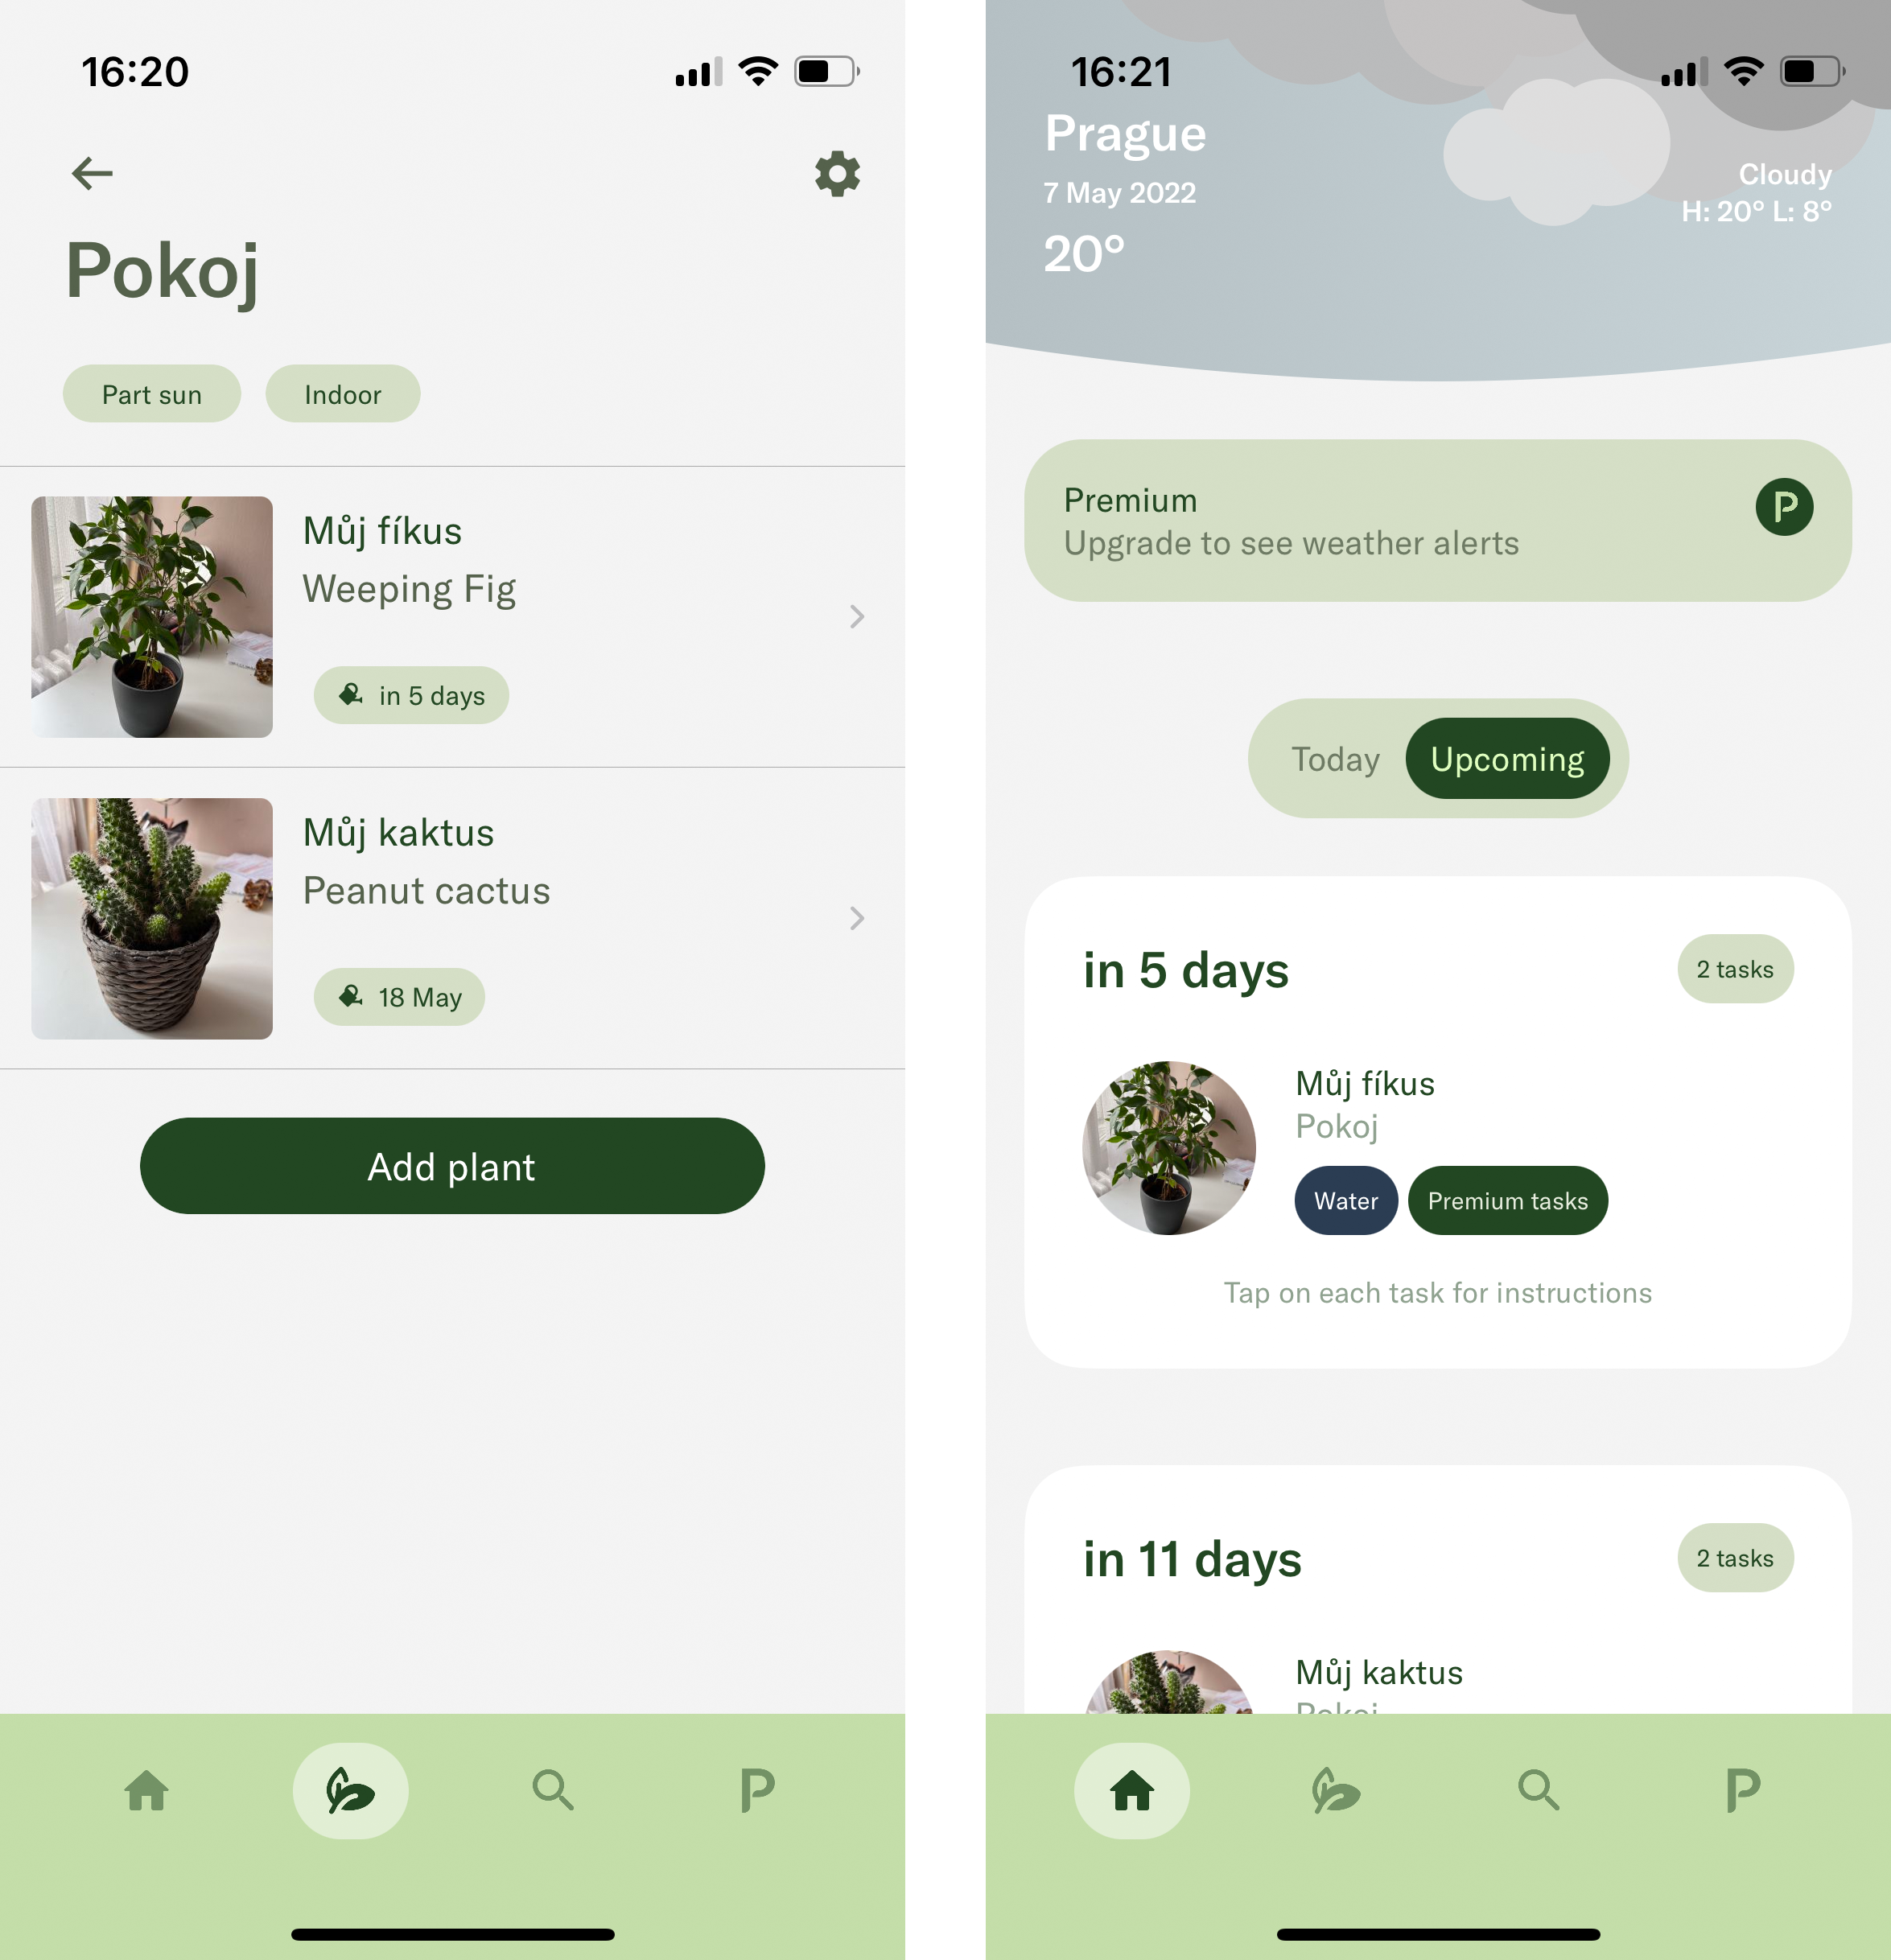
\includegraphics[width=0.75\linewidth]{images/planta.png}
      	\caption{Ukázka aplikace Planta}
      	\label{img:planta}
    \end{figure}

\subsection{PlantIn}
    
    Druhou aplikací je aplikace PlantIn \ref{img:plantin}. Obdobně jako aplikace Planta nabízí uživatelům možnost vytvářet místa/místnosti, do kterých pak můžou ukládat z~dostatečné databáze rostlin. Na detailu rostliny je několik obrázků dané rostliny, pár klíčových informací (toxicita, vhodná teplota, světlo a vlhkost) a následně další užitečné informace v~textové formě. Po přidání rostliny je sestaven plán péče, obdobně jako u~aplikace Planta. Aplikace zohledňuje různé informace (světlo, teplotu, roční období, lokaci) k~modifikace a vytvoření prvotního plánu. Následně si uživatel může manuálně upravit intervaly akcí a povolit/nastavit notifikace. Své rostliny pak lze různě pojmenovávat a změnit jejich výchozí obrázek.
    
    Dále aplikace obsahuje obrazovku s~názvem blog, která nabízí různé články ohledně pěstování, návody nebo různé zajímavosti ze světa rostlin. Aplikace nabízí rozpoznávání rostlin pomocí fotoaparátu. Po úspěšném rozpoznání rostliny se uživatel může dostat na samotný detail rostliny, kde najde již zmíněné informace. Dále také nabízí rozpoznávání nemocí či odbornou pomoc od zkušeného botanisty. Aplikace poskytuje možnost zakoupení prémiového plánu, který nabízí jen pár vylepšení (lepší/chytřejší plán, různé vzhledy/barvy aplikace) od neplacené verze.
    
    Zároveň jako u~aplikace Planta je zde absence spolupráce nebo sdílení rostlin mezi více uživateli. Jinak je aplikace poměrně jednoduchá a hezky vzhledově zpracovaná.
    
    \begin{figure}
    	\centering
    	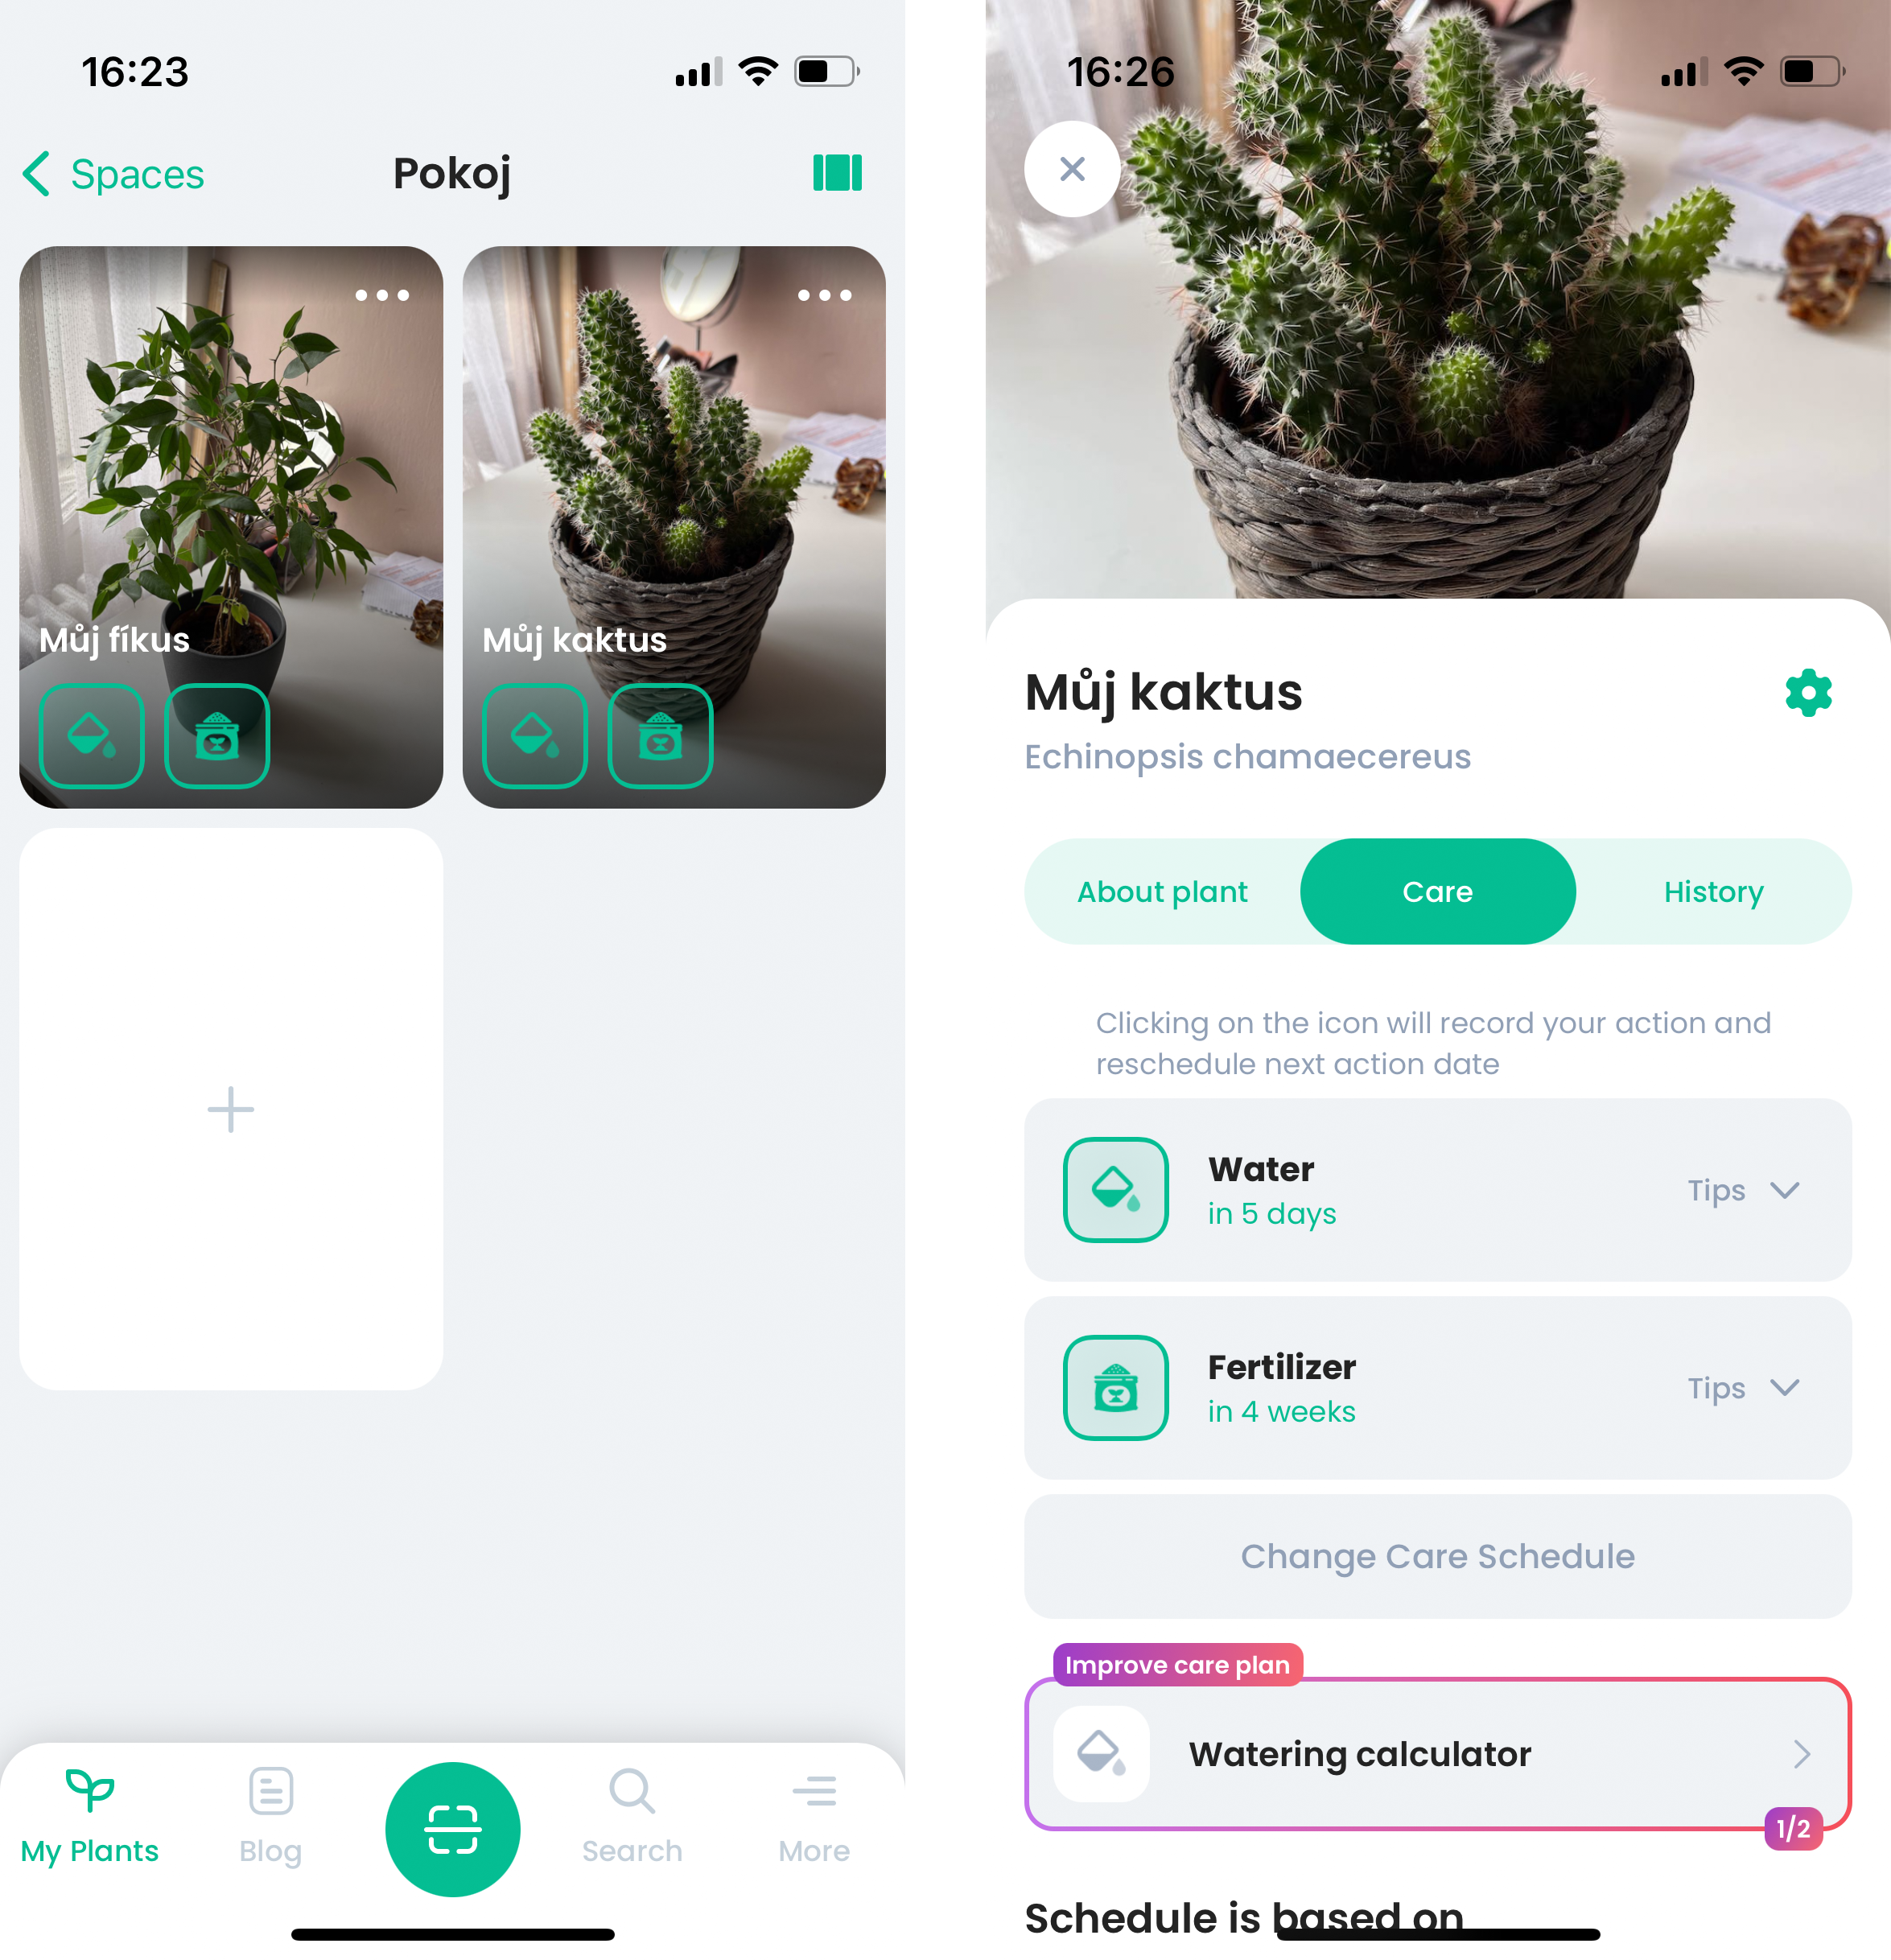
\includegraphics[width=0.75\linewidth]{images/plantin.png}
      	\caption{Ukázka aplikace PlantIn}
      	\label{img:plantin}
    \end{figure}
    
\subsection{Blossom}
    Obdobně jako předchozí aplikace umožňuje aplikace Blossom \ref{img:blossom} vyhledávat z~poměrně obsáhlé databáze rostlin, dále také rozpoznávat rostliny pomocí fotoaparátu. Detail rostliny je vzhledově hezký, na vrchu jsou přehledně zobrazeny nejdůležitější informace, následuje galerie obrázků dané rostliny a poté rozbalovací boxy s~textovými informacemi, které se vztahují k~péči dané rostliny. Rostliny lze přiřadit do uživatelem vytvořených místností. Připomínky/notifikace se nastavují zcela ručně, aplikace nevytvoří sama plán jako u~aplikací Planta a PlantIn. Na druhou stranu je toto ruční nastavení přehledné a umožňuje uživateli plnou kontrolu.
    
    Dalšími funkcemi jsou také, po vzoru předešlých aplikací, rozpoznání chorob/nemocí, odborná pomoc od zkušených odborníků, nabízení článků ohledně pěstování. Aplikace nabízí zakoupení předplatného (prémium), které zpřístupní veškeré funkce aplikace a neomezené rozpoznávání (rostlin a jejich nemocí).
    
    Aplikace je vzhledově dle mého názoru nejpovedenější, ale místy trpí \uv{přeplácaností} prvků, což může být na začátku trochu matoucí. I~zde je absence týmové spolupráce či sledovaní postupu.
    
    \begin{figure}
    	\centering
    	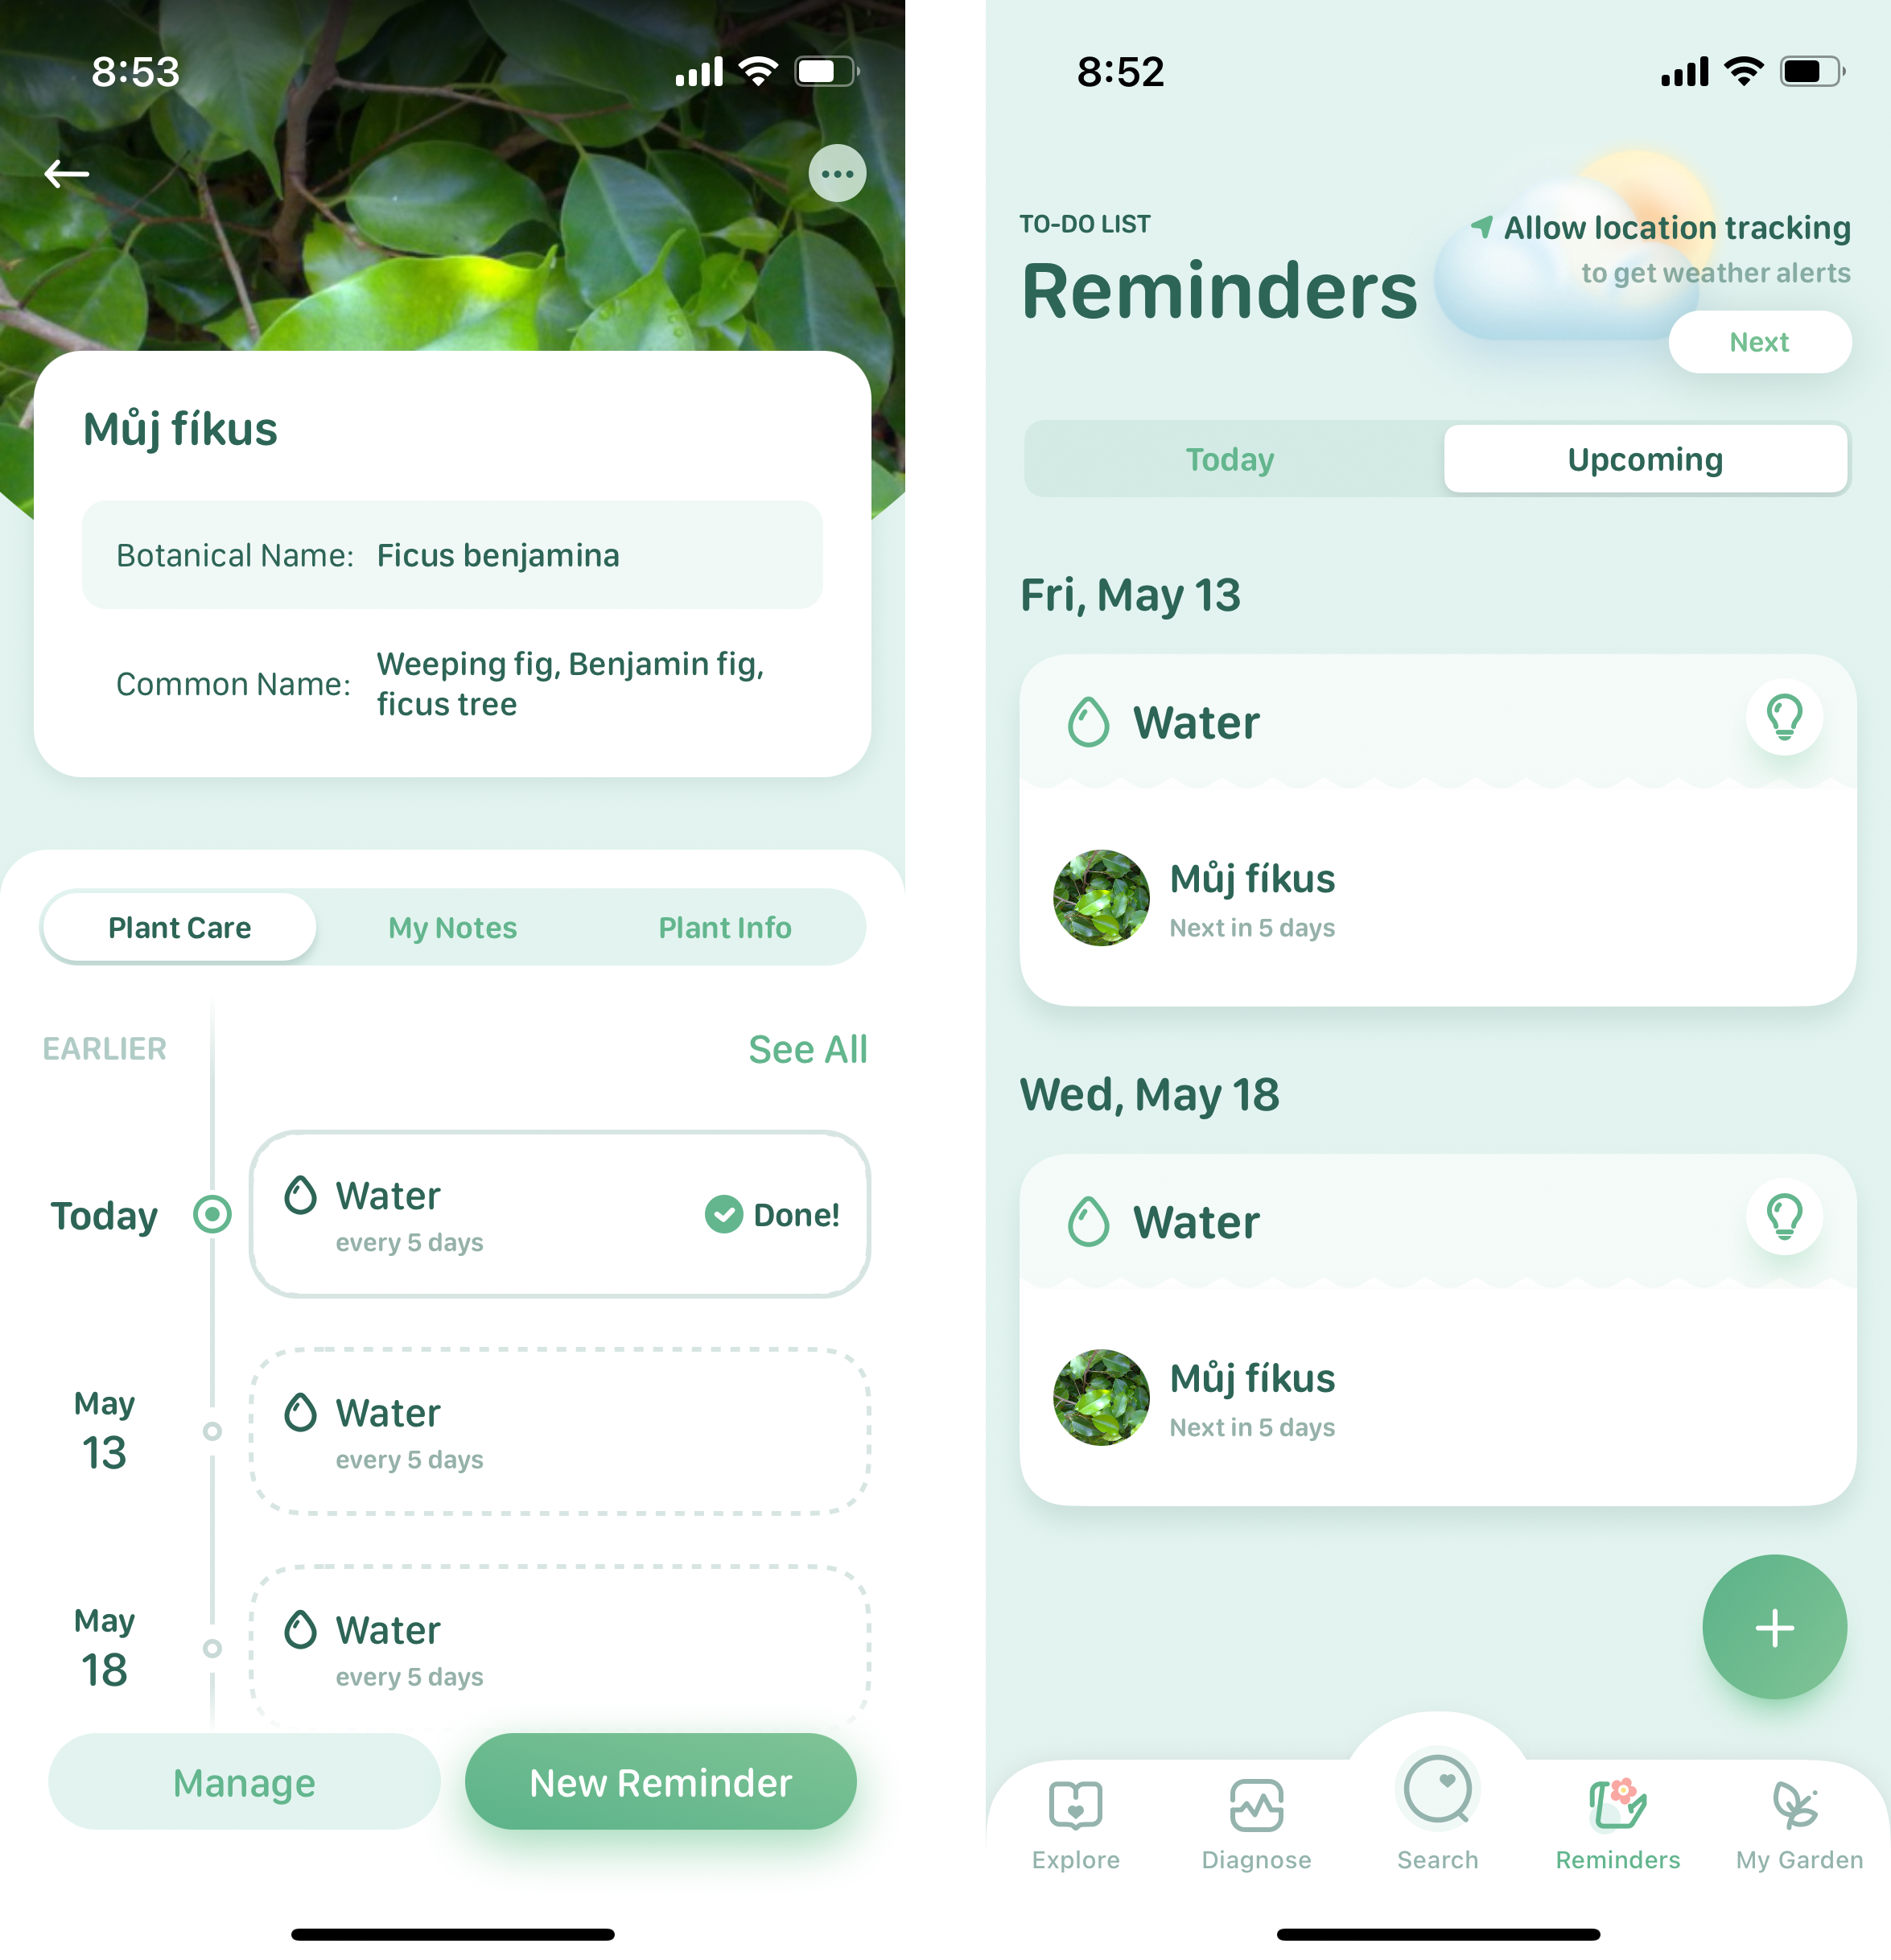
\includegraphics[width=0.75\linewidth]{images/blossom.png}
      	\caption{Ukázka aplikace Blossom}
      	\label{img:blossom}
    \end{figure}
    
\subsection{PictureThis}
    Další aplikací je PictureThis \ref{img:picturethis}. Aplikace jako hlavní funkci nabízí identifikaci rostliny pomocí fotoaparátu, další funkce jsou podobné předchozím aplikacím. Ukládání rostlin, nastavení upomínek na zalévání/hnojení, diagnostiku nemocí či pomoc od expertů. Jedinečnými funkcemi oproti ostatním je rozpoznání hmyzu či ptáků, nicméně toto se netýká tématu.
    
    Opět je zde model zpoplatnění (prémium), které odemkne všechny funkce a odstraní limity. Aplikace opět nenabízí ukládání rostlin v~týmu a sdílení upomínek/postupu.
    
    \begin{figure}
    	\centering
    	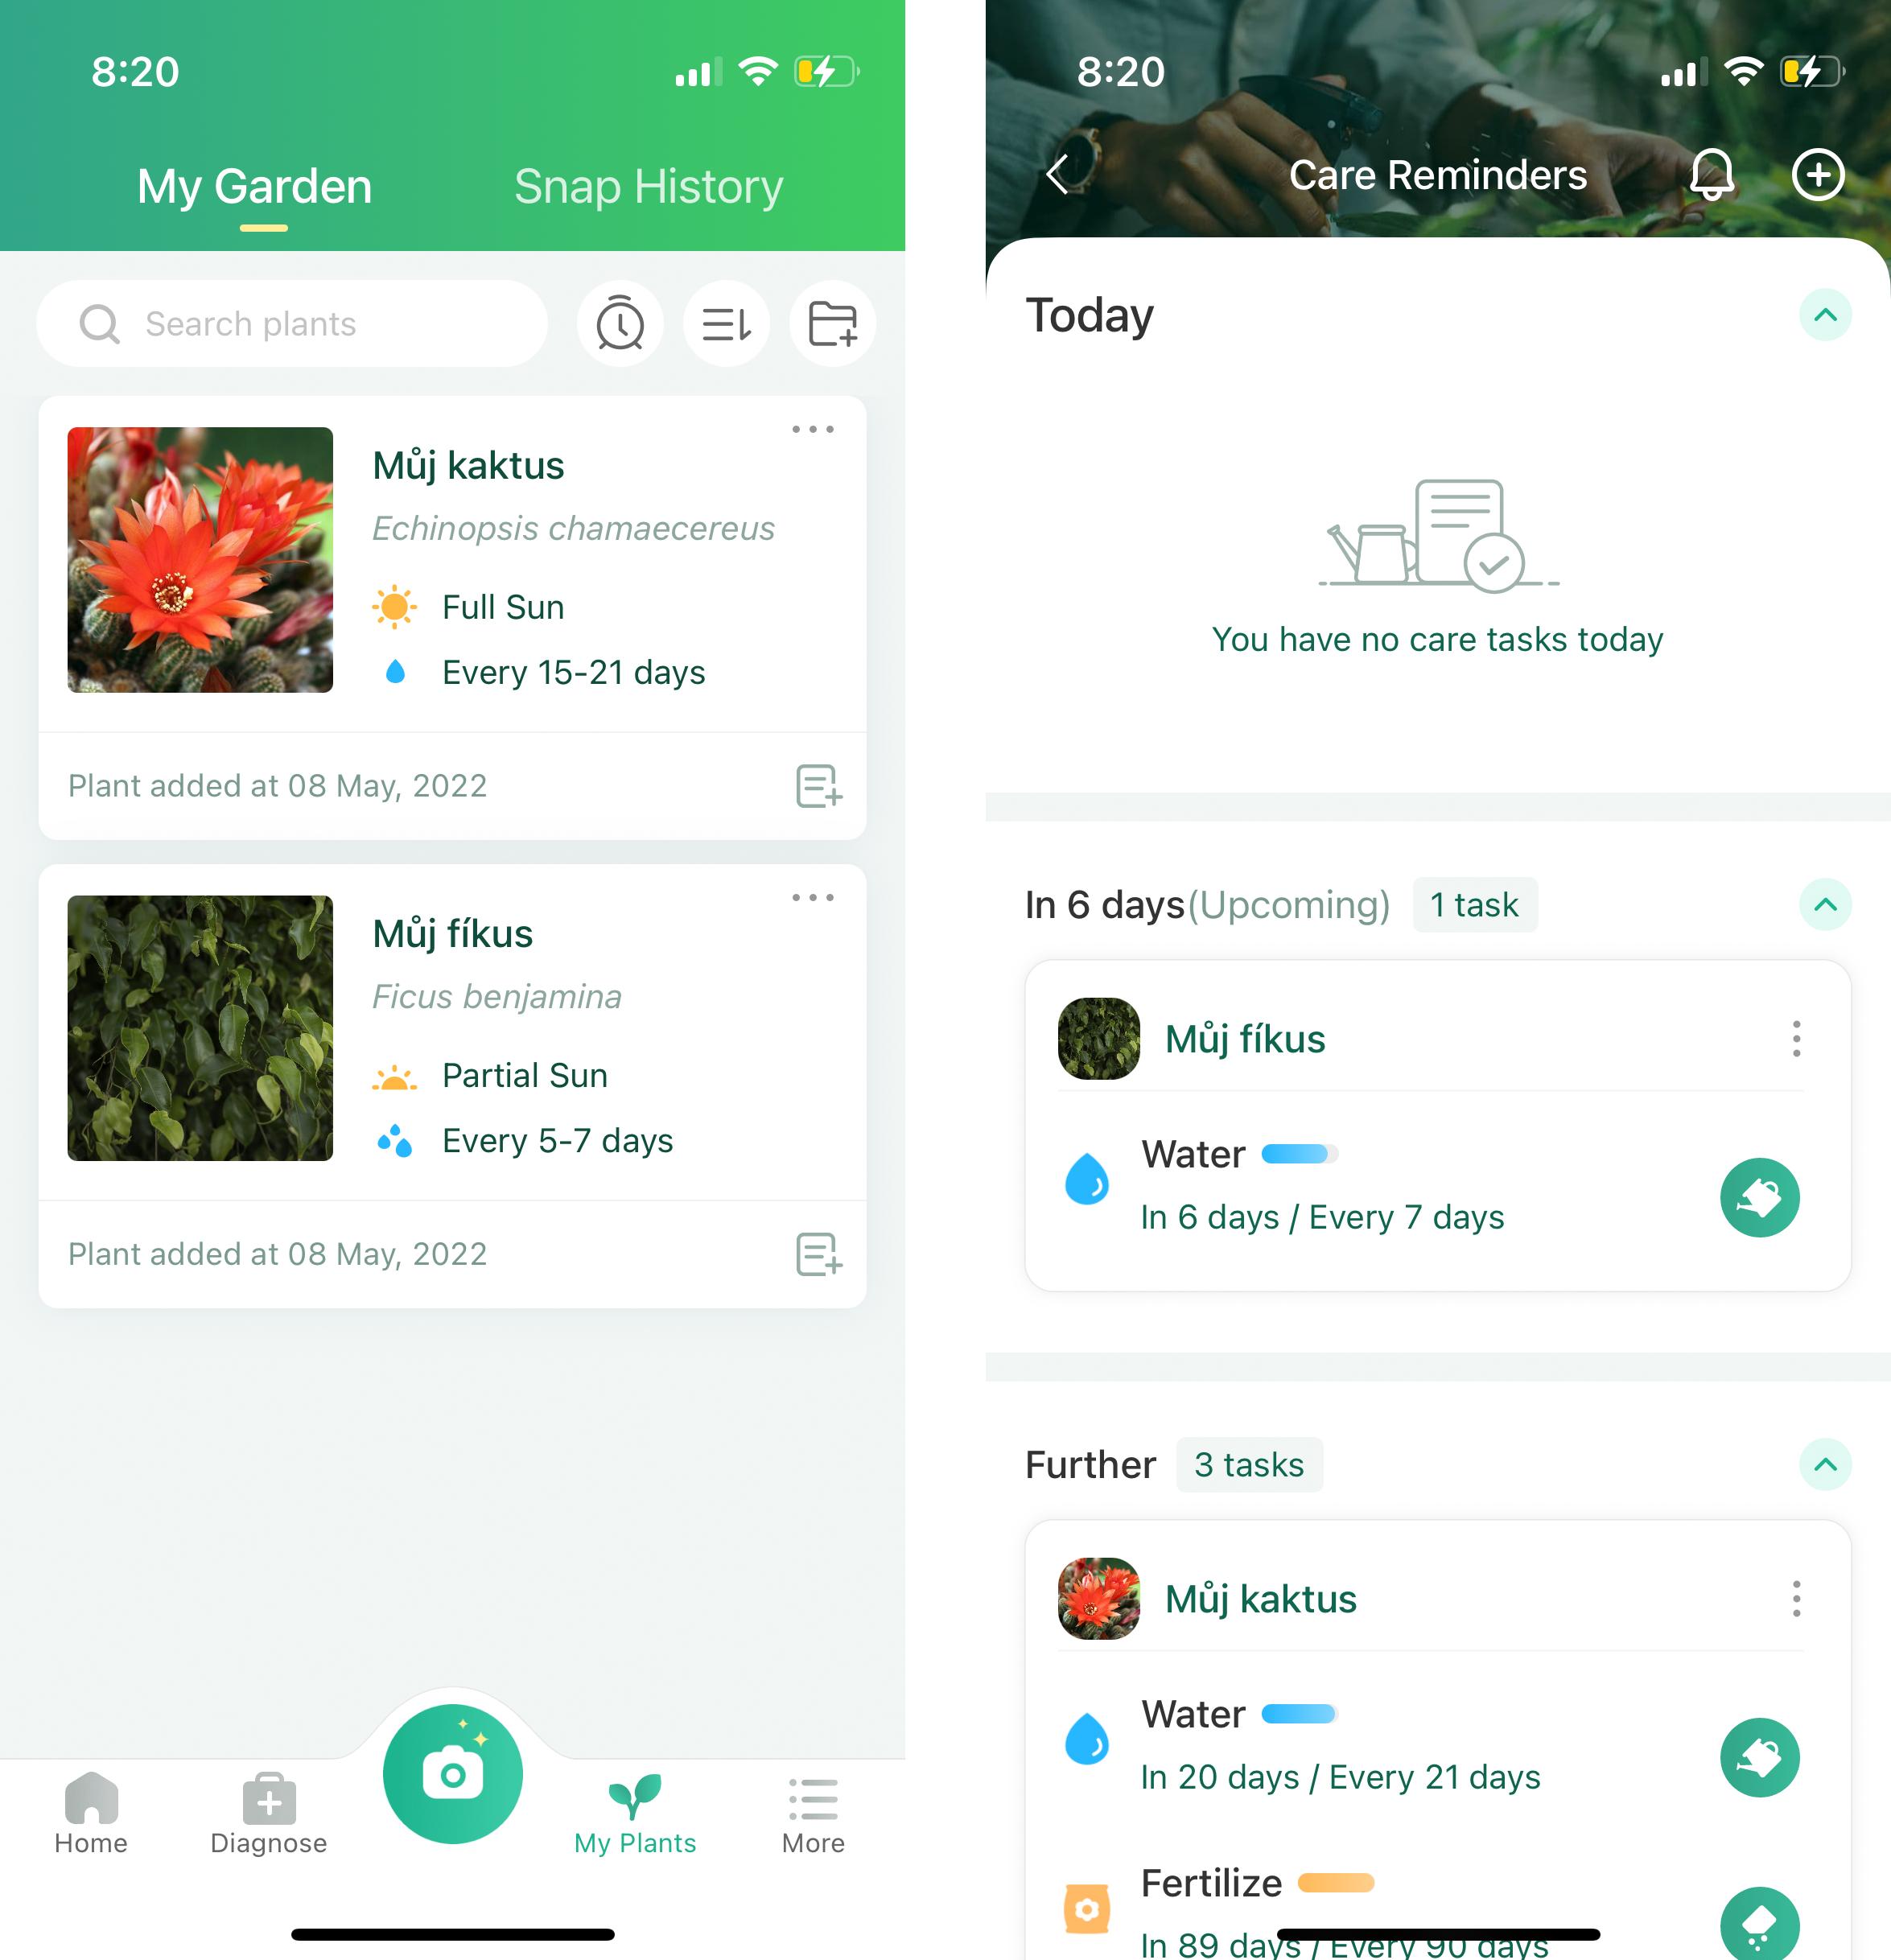
\includegraphics[width=0.75\linewidth]{images/picturethis.png}
      	\caption{Ukázka aplikace PictureThis}
      	\label{img:picturethis}
    \end{figure}
    
\subsection{Florish}
    Aplikace Florish \ref{img:florish} je ukázkou jednoduchosti a minimalismu. Nenabízí z~daleka tolik, co předešlé aplikace. Umožňuje vybírat z~celkem omezené nabídky rostlin a zobrazuje pouze základní informace. Po vložení rostliny může uživatel dostávat připomínky k~zalévání. Dále také umožňuje rozpoznání úrovně světla na daném místě pomocí kamery a vyplnění krátkého dotazníku, na jehož základě umí aplikace doporučit rostlinu uživateli. Na obrazovce \textit{Learn} obsahuje pár článků či návodů ohledně rostlin a péče o~ně. Aplikace je zcela zdarma.
    
    Aplikace sice umožňuje přidávání fotografií rostlin (zřejmě k~rozšíření databáze fotografií), nicméně je u~svých rostlin nelze měnit, stejně tak jako rostliny přejmenovat. Není divu, že se zde nenachází možnost sdílení rostlin více uživatelů mezi sebou. Aplikace je hodně jednoduchá a byla zvolena zejména kvůli zmíněné jednoduchosti a minimalistickému zpracování.
    \newpage
    \begin{figure}[H]
    	\centering
    	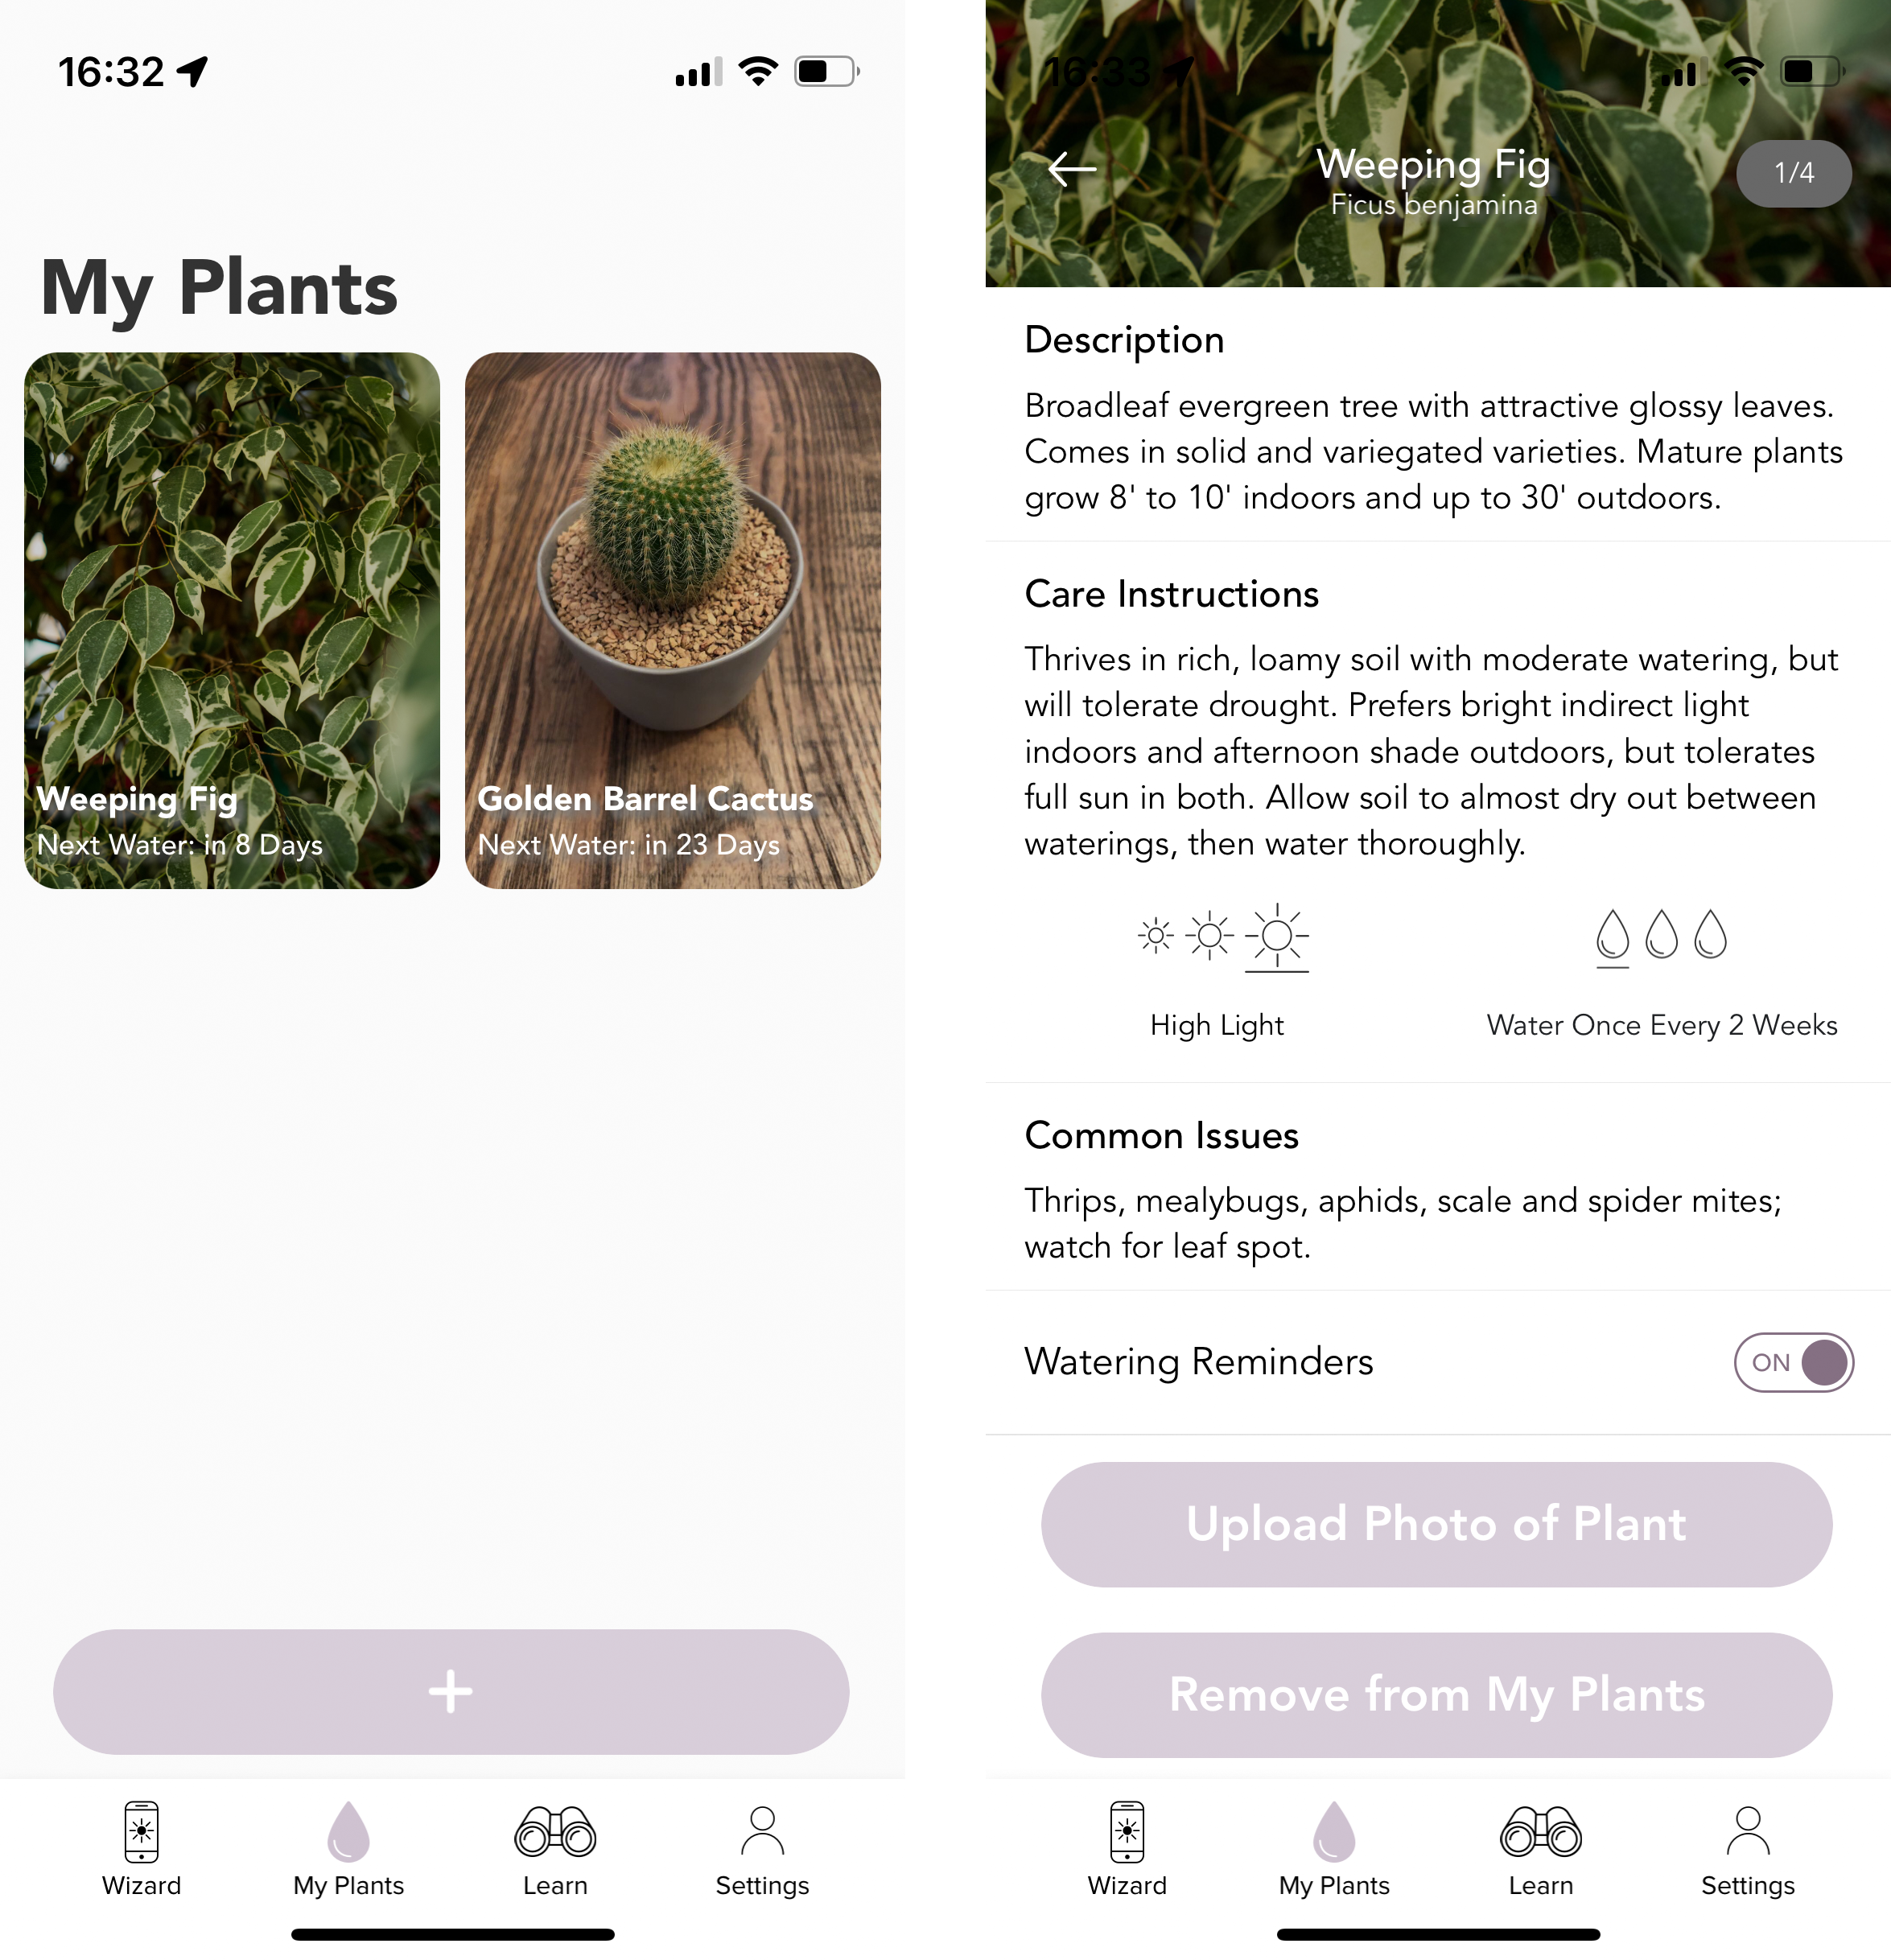
\includegraphics[width=0.75\linewidth]{images/florish.png}
      	\caption{Ukázka aplikace Florish}
      	\label{img:florish}
    \end{figure}
    
\subsection{Ostatní}
    Prozkoumány byly i další aplikace, většina z~nich měla obdobné funkce jako zmíněné aplikace. Zde je jejich výčet:
    \begin{itemize}
        \item Gardenia
        \item Greg
        \item Lovely
        \item PlantPal
        \item Plantnote
    \end{itemize}
    
\subsection{Hodnocení pomocí Nielsenovy heuristiky}
V~tabulce \ref{tab:nielsen} se nachází hodnocení jednotlivých bodů Nielsenovy heuristiky u~každé z~pěti výše podrobněji rozebraných konkurenčních aplikací. Při hodnocení byly udělovány známky na stupnici od 1 (nejlepší) do 5 (nejhorší). Nejlepší hodnocení dosáhla aplikace Planta, která obdržela 21 bodů (méně bodů znamená lepší hodnocení). 22 bodů poté získaly aplikace PlantIn a Blossom. Nejhorší výsledek, 28 bodů, pak patří aplikacím PictureThis a Florish. Uživatelské rozhraní všech hodnocených aplikací vypadá vcelku solidně, žádná vyloženě neobsahuje kritické chyby v~uživatelském návrhu.

\begin{table}[H]
\begin{tabular}{|p{0.26\linewidth}|c|c|c|c|c|}
\hline
                                      & Planta & PlantIn & Blossom & PictureThis & Florish \\ \hline
Viditelnost stavu systému             & 2      & 1       & 2       & 2           & 2       \\ \hline
Shoda mezi systémem a reálným světem  & 1      & 2       & 3       & 3           & 3       \\ \hline
Uživatelská kontrola a svoboda        & 2      & 3       & 2       & 4           & 3       \\ \hline
Konzistence a standardy               & 3      & 2       & 2       & 3           & 2       \\ \hline
Prevence chyb                         & 2      & 2       & 2       & 2           & 4       \\ \hline
Rozpoznání místo vzpomínání           & 2      & 2       & 1       & 3           & 2       \\ \hline
Flexibilita a efektivita              & 2      & 3       & 3       & 2           & 3       \\ \hline
Estetický a minimalistický design     & 2      & 2       & 3       & 3           & 2       \\ \hline
Diagnostika, rozpoznání a oprava chyb & 3      & 2       & 2       & 3           & 3       \\ \hline
Nápověda a dokumentace                & 2      & 3       & 2       & 3           & 4       \\ \hline \hline
Součet                                & 21     & 22      & 22      & 28          & 28      \\ \hline
\end{tabular}
\caption{Tabulka hodnocení konkurenčních aplikací pomocí jednotlivých zásad Nielsenovy heuristiky}
\label{tab:nielsen}
\end{table}
    
\subsection{Souhrn}
Jak je vidět z~analýzy existujících řešení, aplikace mají poměrně vypracované funkce ohledně rozpoznávání rostlin pomocí strojového učení. Některé algoritmus samy spravují, některé používají externí API. Některé aplikace umí sestavit automaticky plán zalévání, či jiných činností v~závislosti na nastavených parametrech uživatele a daných místností.

Tím, čím se bude výsledná aplikace odlišovat, je možnost vytvářet skupiny, ve kterých budou její členové moci provádět a sdílet akce a události. Dále pak budou moci nastavit a dostávat notifikace ohledně různých akcí (zalévání atd.), a to buď jako připomínku nebo přímo notifikaci o~jejím provedení některým ze členů skupiny.

\section{Požadavky}
V~této sekci jsou formulovány požadavky na aplikaci, které vycházejí z~předešlé analýzy. Požadavky se obecně rozdělují do dvou skupin, jimiž jsou požadavky funkční a nefunkční (vysvětlení je popsáno v~\ref{doc:fr} a \ref{doc:nfr}). U~každého požadavku je nutné určit název a stručně ho popsat. Dále je také vhodné přiřadit prioritu, složitost a kategorii. Pro kategorie byl využit model \textit{FURPS}. Pro priority lze využít metodu \textit{MoSCoW}, která jednotlivým požadavkům přiřazuje jednu ze čtyř priorit -- M (Must have), S~(Should have), C (Could have), W (Won't have). Ta však použita nebyla (cílem bylo splnit všechny požadavky) a jednotlivé priority požadavků byly ohodnoceny slovně.

\subsection{FURPS \cite{furps}}
FURPS je zkratka pro Functionality, Usability, Reliability, Performance a Supportability (funkčnost, použitelnost, spolehlivost, výkonnost a podporovatelnost). Právě těchto 5 termínů tvoří jednotlivé kategorie, které se používají pro kategorizaci požadavků na systémy. Model FURPS byl vyvinut ve společnosti Hewlett-Packard, je stále používán v~současnosti a vznikla i jeho modifikace FURPS+, která k~základním pěti kategoriím přidává čtyři další.

\begin{description}
    \item[Funkčnost (Functionality)] Jedná se o~nejdůležitější požadavky. Ty se týkají jednotlivých funkcí, které musí daný systém splňovat. Tedy v~podstatě to, co by měl systém umět a kvůli čemu má být vyvinut/existovat.
    \item[Použitelnost (Usability)] Vypovídají o~schopnosti systému být jednoduše používán uživateli. Jedná se o~vzhled, dojem a vliv na uživatele, přístupnost.
    \item[Spolehlivost (Reliability)] Týkají se spolehlivosti, dostupnosti, předvídatelnosti, přesnosti.
    \item[Výkon (Performance)] Popisují, jak má být systém výkonný a škálovatelný, což zahrnuje jak rychle by měl systém odpovídat, jaké a kolik prostředků bude systém využívat.
    \item[Schopnost být udržována (Supportability)] Věnují se udržitelnosti systému, čili jak je systém čitelný, jaká je zvolena architektura, jestli se dá jednoduše spravovat a provádět modifikace.
\end{description}



\subsection{Funkční požadavky}
\label{doc:fr}
Funkční požadavek (anglicky \textit{functional requirement}, zkratka FR) je specifikace funkce či služby, kterou musí daná aplikace splňovat. Jde o~popis dané funkce, jak se systém bude chovat při daných uživatelských vstupech a jaký bude výsledný výstup. Právě specifikace funkčních požadavků je jedním ze základních pilířů pro návrh aplikace, neboť ujasňuje, co má aplikace dělat a umět. Všechny tyto požadavky spadají do kategorie Funkčnost (Functionality) v~modelu FURPS. \cite{functional-requirements}

Níže jsou vypsány jednotlivé funkční požadavky, včetně názvu, priority, obtížnosti a stručného popisu.

\subsubsection*{FR1 Vytvoření a správa uživatelského účtu}
\textbf{Priorita:} Vysoká \\
\textbf{Složitost:} Vysoká \\

Uživatel se bude moci registrovat nebo se přihlásit. Uživatelský účet pak bude identifikovat jednotlivé uživatele aplikace, budou k~němu přiřazovány jednotlivé týmy, rostliny, provedené akce a další. Svůj uživatelský účet/profil si poté bude moci měnit či upravovat.

\subsubsection*{FR2 Tvorba a správa týmů}
\textbf{Priorita:} Vysoká \\
\textbf{Složitost:} Střední \\

Pro sdílení záznamů o~rostlinách bude klíčové vytvořit funkcionalitu týmové spolupráce. Uživatel bude moci vytvořit tým, do kterého následně může pozvat další uživatele. Společně tak budou mít možnost kooperace či spolupodílení se na péči o~rostliny.

\subsubsection*{FR3 Vyhledávání a zobrazení informací o~rostlinách}
\textbf{Priorita:} Vysoká \\
\textbf{Složitost:} Střední \\

Aplikace bude obsahovat databázi rostlin, přičemž u~každé rostliny se uživatel dozví informace o~ní. Nad touto databází bude možné jednoduše vyhledávat podle jména rostliny (vyhledávací textové pole v~mobilní aplikaci).

\subsubsection*{FR4 Přidávání a správa míst}
\textbf{Priorita:}  Střední \\
\textbf{Složitost:}  Nízká \\

Bude existovat možnost vytvářet, editovat místa, která budou přiřazená jednotlivým záznamům o~rostlině.

\subsubsection*{FR5 Přidávání nových rostlin do svého/týmového seznamu rostlin}
\textbf{Priorita:} Vysoká \\
\textbf{Složitost:}  Střední \\

Na detailu rostliny si uživatel bude moci vybranou rostlinu přidat do své nebo týmové sbírky rostlin. Jedná se o~konkrétní záznam o~rostlině, uživatel může mít více rostlin stejného druhu.

\subsubsection*{FR6 Sledování a správa svých/týmových rostlin}
\textbf{Priorita:} Vysoká \\
\textbf{Složitost:} Vysoká \\

Své nebo týmové rostliny bude moci sledovat, myšleno především události/akce, které byly provedeny nebo jsou naplánovány. Případně bude moci záznam o~rostlině upravit (například uživatelský název).

\subsubsection*{FR7 Přidávání fotek ke svým/týmovým rostlinám}
\textbf{Priorita:} Střední \\
\textbf{Složitost:} Nízká \\

Pro sledování rostlin bude uživatel moci přidávat fotografie, aby měl možnost následně porovnávat růst a vývoj dané rostliny.

\subsubsection*{FR8 Nastavení plánu akcí/událostí}
\textbf{Priorita:} Vysoká \\
\textbf{Složitost:} Vysoká \\

U~každého záznamu rostliny bude uživatel mít možnost nastavit jeden z~připravených plánů nebo si ho sám manuálně sestavit (pomocí vhodných připomínek).

\subsubsection*{FR9 Dostávání a nastavení notifikací}
\textbf{Priorita:} Střední \\
\textbf{Složitost:} Střední \\

Aby uživatel nezapomněl na nějakou akci nebo aby byl informován, že někdo například zalil rostlinu, bude si moci nastavit notifikace.

\subsubsection*{FR10 Zobrazení nadcházejících událostí/akcí}
\textbf{Priorita:} Střední \\
\textbf{Složitost:}  Nízká \\

Uživatel si bude moci zobrazit obrazovku s~přehledem nadcházejících akcí.

\subsection{Nefunkční požadavky}
\label{doc:nfr}
 Nefunkční požadavek (anglicky \textit{non-functional requirement}, zkratka NFR) je požadavek na systém, který se netýká přímo jeho byznysové funkcionality. Typicky se jedná o~kvalitativní parametry systému, může jít například o~dostupnost, použitelnost, responzivita, zabezpečení a další. Jejich specifikace následně ulehčí a ujasní některé věci ohledně samotného vývoje (architektura, technologie). \cite{nonfunctional-requirements}
 
 Zde je vypsán výčet nefunkčních požadavků na aplikaci (název, priorita, obtížnost, kategorie podle FURPS a krátký popis).
 
\subsubsection*{NFR1 Klient-server architektura}
\textbf{Priorita:} Vysoká \\
\textbf{Složitost:} Nízká \\
\textbf{Kategorie:} Schopnost být udržována (Supportability) \\

Jedná se o~jeden ze standardních modelů architektury, kdy server je strana, která spravuje a poskytuje data, která následně zobrazuje a prezentuje klient uživateli (typicky webová, mobilní nebo desktopová aplikace). Tento model architektury bude při návrhu a implementaci výsledné aplikace využit.

\subsubsection*{NFR2 REST API}
\textbf{Priorita:} Vysoká \\
\textbf{Složitost:} Střední \\
\textbf{Kategorie:} Schopnost být udržována (Supportability) \\

Server bude komunikovat s~mobilní aplikací pomocí protokolu HTTP s~využitím architektonického vzoru REST.

\subsubsection*{Mobilní aplikace pro systém iOS}
\textbf{Priorita:} Vysoká \\
\textbf{Složitost:} Vysoká \\
\textbf{Kategorie:} Schopnost být udržována (Supportability) \\

Klientská část aplikace bude implementována pro mobilní aplikace s~operačním systémem iOS, tedy pro mobilní zařízení od společnosti Apple.

\subsubsection*{NFR4 Jednoduchost používání aplikace}
\textbf{Priorita:} Střední \\
\textbf{Složitost:} Vysoká \\
\textbf{Kategorie:} Usability (Použitelnost) \\

Bude kladen důraz, aby byla mobilní aplikace jednoduchá na používání, což lze zajistit vhodným návrhem vzhledu a správným a logickým propojením obrazovek pomocí interakčních prvků.

\subsubsection*{NFR5 Svižnost aplikace}
\textbf{Priorita:} Střední \\
\textbf{Složitost:} Střední\\
\textbf{Kategorie:} Výkon (Performance) \\

Ideálně by aplikace neměla mít dlouhé odezvy v~komunikaci a obecně se zasekávat. Aplikace by rozhodně neměla padat a v~případě problému zobrazovat smysluplné hlášky.

\subsubsection*{NFR6 Vysoká dostupnost serveru}
\textbf{Priorita:} Střední \\
\textbf{Složitost:} Nízká \\
\textbf{Kategorie:} Spolehlivost (Reliability) \\

Mobilní aplikace by měla být schopna zobrazovat data neustále (kdykoliv na požádání), je tedy potřeba, aby byl server dostupný ideálně 24/7.

% --------------------------------------------------------------------------------------------

\chapter{Metodiky vývoje software}
Softwarový vývoj není jednoduchá disciplína. Jedná se o~poměrně složitý proces, který se skládá z~mnoha podprocesů/částí. Ty zároveň nejsou striktně dány, neboť každý vývojový proces se liší, především podle vyvíjeného produktu. Proto se v~průběhu let začaly vytvářet různé metodiky pro vývoj software, které popisují vhodné systematické kroky a postupy při vývoji. Cílem těchto metodik je především zjednodušení samotného vývoje, ve smyslu poskytnutí jasné struktury. Vhodná struktura přináší větší efektivitu, přehlednost, kontrolu a usnadňuje plánování a komunikaci. Je ovšem nutné nevybrat slepě určitou metodiku jen proto, že patří mezi aktuální trendy nebo proto, že ji používá ona společnost při jejich vývoji. Volba by měla brát v~potaz přímo daný produkt (rozsáhlost, požadavky, technologie atd.), jenž má být vyvinut, a také tým, který se bude na vývoji podílet (velikost, preference, zkušenost atd.). Zároveň každá metodika má svoje kladné i záporné stránky. V~následujících sekcích jsou popsány nejznámější a nejpoužívanější metodiky. \cite{software-development-methodologies-1, software-development-methodologies-2}

\section{Waterfall \cite{waterfall}}
Jednou z~prvních a zároveň také jednou z~nejpoužívanějších metodik je \textit{Waterfall}, v~překladu vodopádový model. Jedná se o~sekvenční vývojový model, který je rozdělen do několika hlavních fází (jejich počet se může lišit, standardně se jich uvádí 5), přičemž každá závisí na té předchozí (lze si představit vodopád s~jednotlivými patry, viz obrázek \ref{dia:waterfall}) a nelze se vracet zpět. Jednotlivé fáze jsou:

\begin{description}
    \item[Requirements (Požadavky)] Fáze, při které dochází k~analýze, specifikaci požadavků a definici funkcí, které má výsledný produkt obsahovat.
    \item[Design (Návrh)] Vývojový tým, vzhledem k~požadavkům (z~předchozí fáze) definuje vhodnou softwarovou architekturu, vybírá vhodné technologie.
    \item[Implementation (Implementace)] Na základě návrhu je software/produkt implementován.
    \item[Verification (Verifikace)] V~této fázi je ověřeno a otestováno, zda je implementace funkční a odpovídá všem požadavkům, které byly specifikovány. Zároveň je také daná implementace vydána.
    \item[Maintenance (Údržba)] Vydáním produktu ovšem práce většinou nekončí. V~této fázi jde o~dodatečné testování, opravu nově vzniklých problémů či údržbu a upgrade strojů.
\end{description}

\subsection*{Výhody}
\begin{itemize}
    \item Linearita přispívá k~snadnějšímu pochopení, zejména pro nové vývojáře.
    \item Všechny specifikace a výstupy jsou popsány před zahájením vývoje.
    \item Protože je vše jasně definováno a popsáno v~každé fázi, není zde prostor pro špatnou komunikaci informací.
\end{itemize}

\subsection*{Nevýhody}
\begin{itemize}
    \item Riziko odchýlení projektu od cíle z~důvodu absence zpětné vazby od zákazníků v~počátečních fázích.
    \item Testování probíhá až na konci vývoje. Některé chyby, které zejména vznikly na počátku vývoje, mohou být problematické na opravu.
    \item Striktnost a malá flexibilita metodiky není vhodná pro komplexnější projekty.
    \item Důraz na dokumentaci místo dodávání řešení, která řeší problémy uživatelů.
\end{itemize}

\begin{figure}
	\centering
	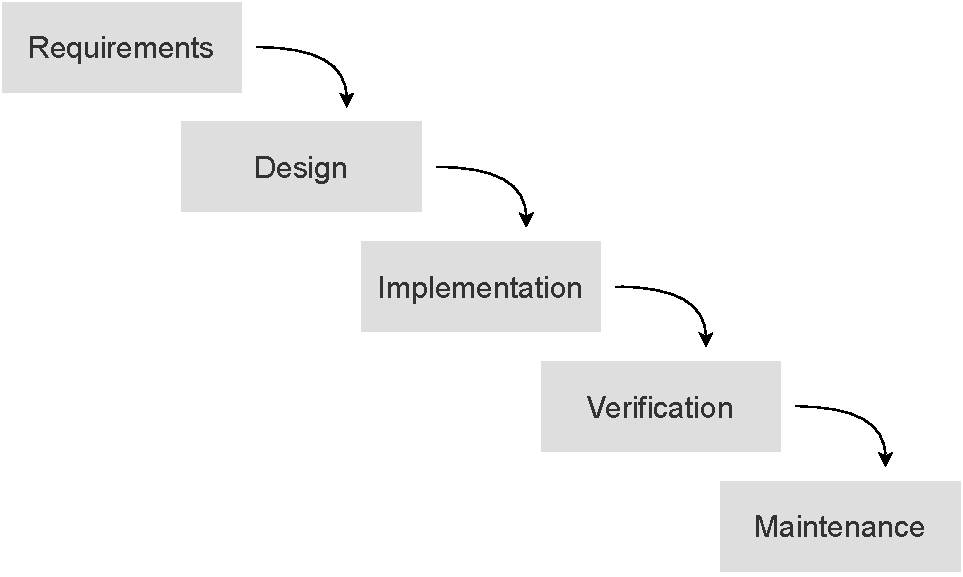
\includegraphics[width=0.7\linewidth]{images/waterfall.pdf}
  	\caption{Znázornění metodiky Waterfall}
  	\label{dia:waterfall}
\end{figure}

\section{Agile \cite{agile}}
Agilní metodiky patří v~poslední době k~nejvíce populárním metodikám. Místo lineárního postupu, jako u~vodopádové metodiky, se soustředí na správnou komunikaci se zákazníkem a uspokojování jeho potřeb. Nelpí tolik na tvorbě dokumentace a dodržování striktních postupů. Vývoj probíhá v~tzv. sprintech, které zpravidla trvají 1 - 4 týdny. V~těchto sprintech se vyvíjí dílčí části produktu, které berou v~potaz podněty zákazníka a zároveň se průběžně testuje. Tyto sprinty se neustále opakují, jedná se tedy o~iterativní proces. V~průběhu času vznikly různé modifikace a zpřesnění této metodiky, například Scrum a další.

\subsection*{Výhody}
\begin{itemize}
    \item Minimum chyb díky opakovanému testování a ladění. 
    \item Častá komunikace se zákazníkem umožňuje rychle reagovat na jeho požadavky a řešit případné problémy.
    \item Dosažení kvalitnějšího konečného výsledku.
\end{itemize}

\subsection*{Nevýhody}
\begin{itemize}
    \item Časová náročnost kvůli časté komunikaci 
    \item Díky nedůrazu na dokumentaci může být vývoj v~pozdějších fázích problematičtější.
    \item Ztráta soustředěnosti kvůli častým požadavkům.
    \item Díky nestrukturovanému přístupu jsou potřeba zkušení a nezávislí vývojáři.
\end{itemize}

\section{Scrum \cite{scrum}}
Tato metodika spadá pod agilní metodiky a patří mezi nejflexibilnější. Dodržuje agilní koncepty a rozděluje vývojový tým do rolí. První rolí je Product Owner (vlastník produktu). Ten je zodpovědný za komunikaci s~klientem a zajišťuje, že vývojový tým dodržuje termíny a doručuje požadované funkcionality. Dále se v~týmu nacházi Scrum Master, který slouží jako prostředník mezi vlastníkem produktu a vývojovým týmem. Ten má zároveň za cíl zajistit správný chod scrum procesu, odstiňuje ostatní členy týmu od negativních vlivů, organizuje schůzky/porady a povzbuzuje tým. Vývojový tým (obvykle 3 - 9 vývojářů) pak pracuje na aktuálním inkrementu daného sprintu. Součástí scrum procesu je plánování nadcházejícího sprintu a denní scrumy (krátké porady).

\begin{figure}
	\centering
	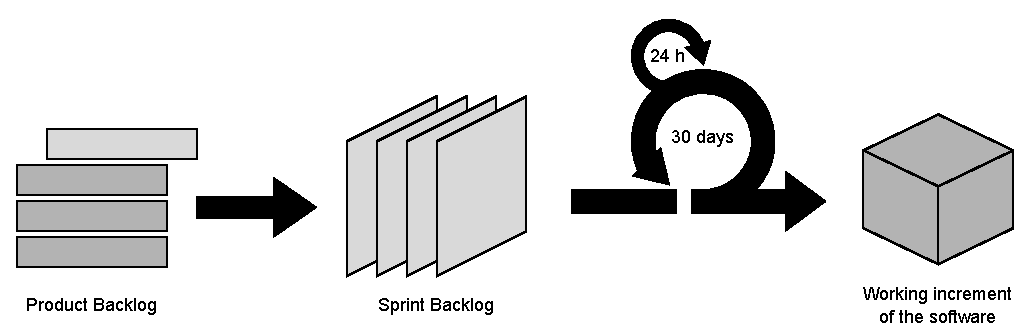
\includegraphics[width=1\linewidth]{images/scrum.pdf}
  	\caption{Znázornění metodiky Scrum}
  	\label{dia:scrum}
\end{figure}

\subsection*{Výhody}
\begin{itemize}
    \item Časová a ekonomická efektivita.
    \item Krátké iterace umožňují rychle reagovat na požadavky klienta.
    \item Pravidelné schůzky/porady zajišťují, že všichni členové ví, co se zrovna děje a kdo na čem pracuje.
\end{itemize}

\subsection*{Nevýhody}
\begin{itemize}
    \item Nutnost zkušených vývojářů a také odhodlanost následovat metodiku scrum.
    \item Denní scrum porady mohou být pro vývojáře frustrující.
    \item Nevhodné pro rozsáhlé projekty.
\end{itemize}

\section{Feature Driven Development (FDD) \cite{fdd}}
Stejně jako scrum, tato metodika je založena na agilním přístupu. Hlavní myšlenkou je vytvoření základního systémového modelu, ze kterého je poté vytvořen seznam funkcí (feature list). Separátně se poté na každé funkci prochází plánováním, návrhem a samotným vývojem. Práce na jednotlivých funkcí by zpravidla neměla trvat déle než 2 týdny.

\subsection*{Výhody}
\begin{itemize}
    \item Dá se pracovat na více funkcích zároveň a díky tomu je tato metodika vhodná pro rozsáhlé projekty.
    \item Rozdělení komplikovaných úloh na menší, což vede k~větší efektivitě.
    \item Není potřeba častých porad/schůzek, komunikace především v~textové formě.
\end{itemize}

\subsection*{Nevýhody}
\begin{itemize}
    \item Nevhodné pro malé projekty.
    \item Závislost na hlavním vývojáři, který má kromě vývoje na starost i distribuci a koordinaci úloh mezi ostatní vývojáře.
    \item Absence kvalitní dokumentace.
\end{itemize}

\section{Prototyping \cite{prototyping}}
Tato metodika je založena na vytvoření prototypu aplikace (základní klíčové funkce), který je poté dokola testován a přepracováván do té doby, než je dosaženo přijatelného výsledku. Postupuje se zpravidla tak, že ze začátku se specifikují požadavky, dojde k~rychlému návrhu a následnému vytvoření prototypu (základní klíčové funkce, není dokonalý). Poté dochází k~již zmiňovaným cyklům testování a znovuvytváření lepšího prototypu. Nakonec je finální produkt řádně otestován, nasazen do produkce a následně je prováděna údržba. Pro úplnost je třeba dodat, že existují různé varianty této metodiky (\textit{rapid throwaway}, \textit{evolutionary}, \textit{incremental}, \textit{extreme}), které se liší ve vlastnostech prototypů nebo způsobem, jakým jsou vytvářeny.

\subsection*{Výhody}
\begin{itemize}
    \item Přímočará metodika, jednoduchá na pochopení.
    \item Klient velmi brzy vidí \uv{nějaký} výsledek a může hned poskytovat zpětnou vazbu. Zároveň se tak dají brzy podchytit potenciální problémy.
\end{itemize}

\subsection*{Nevýhody}
\begin{itemize}
    \item Celý proces vytváření, testování, vylepšování je značně časově náročný.
    \item Klient může z~dosavadních prototypů nabýt představy, že produkt je téměř hotový, nebo naopak přestane mít zájem ho dodělat, protože není s~dosavadním výsledkem spokojený.
    \item Zaostávající dokumentace z~důvodu častých změn požadovaných od zákazníka.
\end{itemize}

\begin{figure}[H]
	\centering
	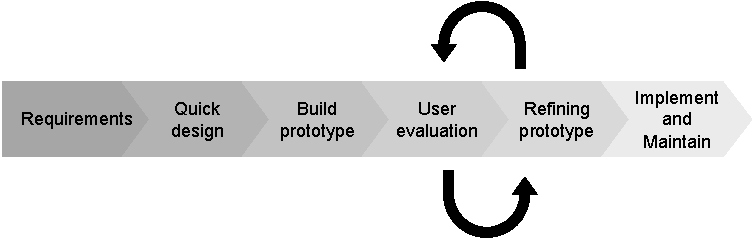
\includegraphics[width=1\linewidth]{images/prototyping.pdf}
  	\caption{Znázornění metodiky Prototyping}
  	\label{dia:prototyping}
\end{figure}

\section{Lean \cite{lean}}
Tato metodika se zrodila ve firmě Toyota a stojí na dvou základních pilířích. Prvním je vytváření nových funkcí či provádění změn, které přináší největší hodnotu, zaberou nejméně úsilí a času. Zadruhé je kladen důraz na respektování lidí. Lean se mimořádně hodí při přepracovávání již hotových, zejména dlouho používaných projektů (přechod na nové technologie, předělání uživatelského rozhraní atd.).

\subsection*{Výhody}
\begin{itemize}
    \item Minimální životaschopný produkt (MVP) je dodán poměrně rychle.
    \item Náklady na vývoj jsou poměrně nízké.
\end{itemize}

\subsection*{Nevýhody}
\begin{itemize}
    \item Nutnost precizní dokumentace a její porozumění.
    \item Vyžaduje velmi zkušené jednotlivce s~dostatečnými znalostmi. Nelze se učit \uv{za pochodu}, neboť to přináší risk.
\end{itemize}

\section{Spiral \cite{spiral}}
Ve spirálové metodice se proces vývoje skládá ze čtyř fází. Vývojáři těmito fázemi průběžně procházejí ve spirále/cyklu. Po každém průchodu postupují do nové iterace vývoje, přičemž cílem je v~každé iteraci postupně zdokonalovat produkt.

\begin{description}
    \item[Plánování] Definice cílů v~dané fázi vývoje.
    \item[Analýza rizika] Snaha o~předvídání rizika a snaha navrhnout jejich řešení.
    \item[Vývoj] Návrhu a vývoj produktu na základě předchozích fází.
    \item[Vyhodnocení] Vyhodnocení stavu projektu a plánování další iterace.
\end{description}

\subsection*{Výhody}
\begin{itemize}
    \item Možnost vyhnout se riziku díky důkladné analýze.
    \item Velká flexibilita.
    \item Vhodné pro velké projekty.
    \item Prostor pro zpětnou vazbu od zákazníků.
\end{itemize} 

\subsection*{Nevýhody}
\begin{itemize}
    \item Použití této metodiky může být dosti nákladné.
    \item Úspěch projektu je závislý na analýze rizik, která zároveň vyžaduje odborné znalosti.
    \item Nefunguje příliš dobře pro menší projekty.
\end{itemize}

\begin{figure}
	\centering
	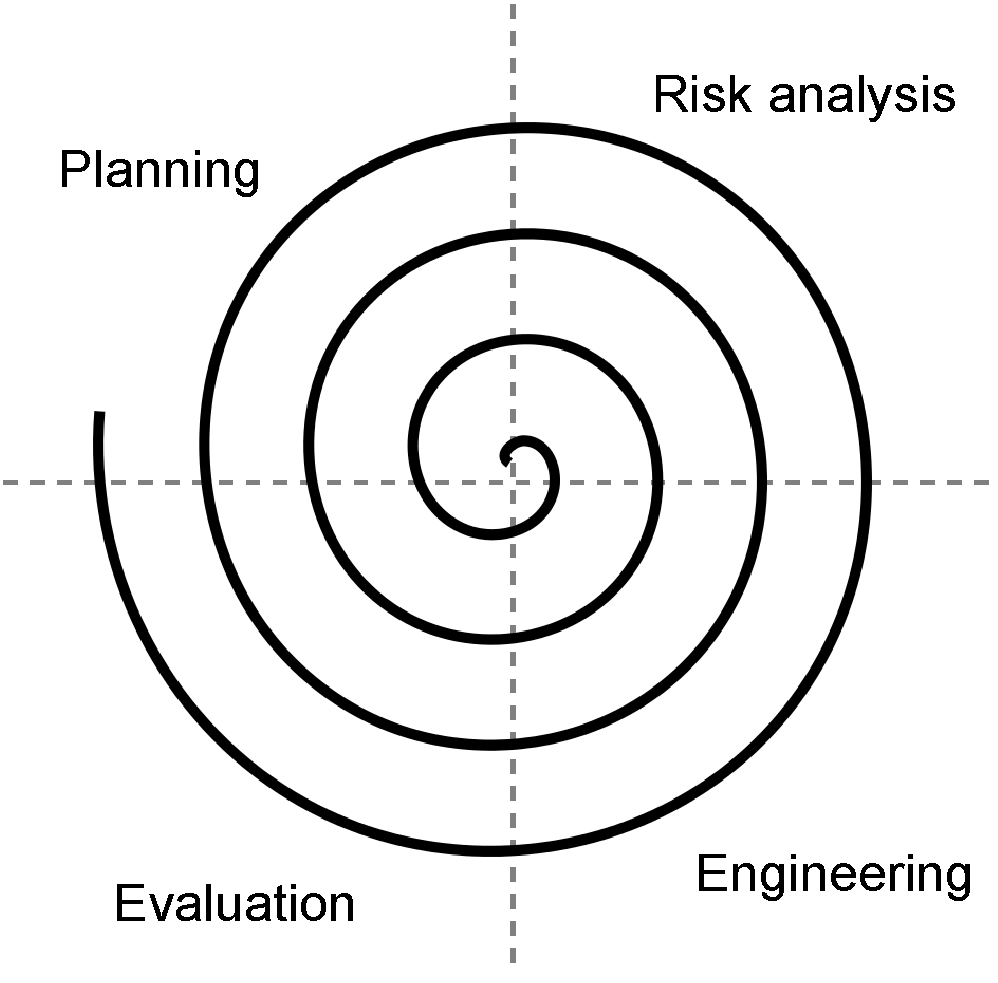
\includegraphics[width=0.5\linewidth]{images/spiral.pdf}
  	\caption{Znázornění metodiky Spiral}
  	\label{dia:spiral}
\end{figure}

\section{Výběr metodiky}
Důležitým faktorem, který hrál roli ve výběru metodiky, je jednočlenný vývojový tým (já, autor této práce). Není tak nutné řešit spolupráci mezi více lidmi. Nejedná se zároveň o~komplexní projekt a náklady na vývoj jsou nízké (převážně jen čas a zaplacení služeb pro finální nasazení). I~z~důvodu přímočarosti, jasné struktury a snadné uchopitelnosti byla použita především vodopádová metodika (Waterfall), která je místy podle potřeby lehce obohacena o~prvky jiných metodik.

% --------------------------------------------------------------------------------------------

\chapter{Návrh}

\section{Persony}
Personou se rozumí smyšlená fiktivní osoba, která reprezentuje uživatele aplikace. Persony slouží k~vytvoření představy, co uživatel chce, jaké má potřeby, jaké jsou jeho cíle či jak se uživatel bude chovat. Pomáhají tak identifikovat uživatele, kteří aplikaci budou hojně využívat, či uživatele, pro které aplikace vhodná není. Při vytváření person jde o~zobrazení uživatele, která reprezentuje vytyčenou skupinu lidí. Typicky se tvoří 3 různé persony, přičemž jde o~typického a příležitostného uživatele a uživatele, který aplikaci téměř nepoužije (negativní uživatel). Persona by měla působit jako reálný člověk, dává se jí jméno, věk, pohlaví a dále také jaké jsou třeba její záliby, historie a typický den. \cite{personas-1, ui-design-steps}

\subsection{Persona A~- typický uživatel}
\begin{description}
    \item[Jméno] Jana Nováková
    \item[Věk] 29
    \item[Pohlaví] Žena
    \item[Koníčky] vaření, cestování, pěstování rostlin
    \item[Životní historie] Jana je pracovitá, energická, milující matka a manželka. Žije v~malém domku na okraji Prahy. Naplno využívá svůj volný čas. Dělá zásadně činnosti, které ji baví. To, co ji nebaví, přenechává ostatním. Ráda se učí novým věcem. Ve volném čase ráda sportuje, vaří a stará se o. Jana vystudovala střední obchodní školu. Ihned po škole začala pracovat v~marketingové agentuře. Následně odešla na mateřskou dovolenou, přičemž po ní se vrátila zpět do předešlé práce. Nyní aspiruje na pozici vedoucí oddělení.
    \item[Typický den] Jana vstává okolo šesté hodiny, spolu jako rodina se nasnídají, připraví se a vypraví se autem do práce, kde cestou vysadí svého syna ve školce. Cestou z~práce syna ve školce opět vyzvedne a spolu dorazí domů. Zbytek dne Jana tráví se svým synem a manželem doma. Jako vášnivý pěstitel rostlin se často (mimo zimní období) pohybuje po jejich menší zahrádce, na které spolu pěstují nejrůznější druhy rostlin a květin. Také uvnitř jejich domu lze nalézt velké množství pokojových rostlin. Občas ji přijde, že rostlin má přehršel a stane se jí, že se o~ně nestíhá starat, nebo že na nějakou sem tam zapomene.
\end{description}

\subsection{Persona B - příležitostný uživatel}
\begin{description}
    \item[Jméno] Petr Klíč
    \item[Věk] 46
    \item[Pohlaví] Muž
    \item[Koníčky] fotbal, auta
    \item[Životní historie] Petr už má něco za sebou, leccos ho už nepřekvapí. Má své zajeté koleje, ale zároveň se nebrání vyzkoušet i něco nového. Používá aktivně chytrý telefon, který mu slouží hlavně jako komunikační zařízení. Ve svém bytě má pár pokojových rostlin, které sporadicky (když si vzpomene) zalije. Už několikrát se mu stalo, že zapomněl zalít svůj fíkus, a tak mu v~létě uschl.
    \item[Typický den] Petr je mužem středního věku, je otcem dvou dětí. Petr žije sám, s~manželkou se rozvedl, když mu bylo 36 a děti už se odstěhovaly do vlastního. Bydlí ve větším městě v~menším bytě a kousek od něj vlastní garáž. Každý pracovní den vstává v~půl sedmé ráno, nasnídá se, pustí si ranní zprávy v~televizi a následně jde do zaměstnání (provozní elektrikář). Obědvá v~práci a domů se vrací kolem čtvrté. Po práci chodí dvakrát týdně hrát s~přáteli rekreačně fotbal, či se stará v~garáži o~své milované auto. Večer občas zajde s~přáteli na pivo do hospody nebo sleduje fotbalová utkání v~televizi. O~víkendech odpočívá a jezdí za ním na návštěvu děti.
\end{description}

\subsection{Persona C - negativní uživatel}
\begin{description}
    \item[Jméno] Helena Dvořáková
    \item[Věk] 72
    \item[Pohlaví] Žena
    \item[Koníčky] televize, procházky v~přírodě
    \item[Životní historie] Helena je pesimistická, poctivá a obětavá důchodkyně. Nerada se učí nové věci. Nerada mění své názory. Je přesvědčená, že si za svůj život všechny své názory na svět vytvořila a nechce je již měnit. Helena vystudovala učitelství a celý svůj život učila na druhém stupni základní školy zeměpis a dějepis. Vždy byla vnímána ve škole jako ta \uv{hodná} učitelka. Žije sama v~malém domku na okraji malého městečka. Manžel ji bohužel před pár lety umřel při autonehodě.
    \item[Typický den] Helena vstává ráno kolem šesté hodiny. Připraví si snídani a sní si ji v~doprovodu ranních televizních zpráv. Dopoledne obvykle tráví doma, kouká na televizi či si čte noviny. Pokud nemá připravený oběd z~předešlých dní, tak si ho s~dostatečným předstihem uvaří a pak ho následně sní. Po obědě vyráží na krátkou procházku do přírody nebo se jde starat o~svoji zahrádku, neboť si ji chce ještě užít, dokud může. Večer tráví buď sama u~televize nebo chodí na návštěvy k~jejím přátelům, kde rozebírají nejrůznější věci, které se staly. O~víkendech za ní jezdí příbuzní.
\end{description}

\section{Případy užití a scénáře}

Význam termínu případ užití (anglicky \textit{use case}) má široké pojetí. Ve vývoji softwaru lze jednoduše říci, že jde v~podstatě o~specifikaci a popis klíčové funkcionality aplikace. Tento popis je vytvořen na základě cílů, kterého chce daná entita dosáhnout (typicky uživatel nebo systém), a je reprezentován sadou kroků, které vedou k~jejich dosažení. Jednotlivé případy užití by měly ideálně popisovat pouze jednoduché akce/činnosti. Samotný formát, jak mají případy užití vypadat, není striktně daný, níže je použit tzv. Fowlerův styl. Ten obsahuje název, krátký popis a jednotlivé scénáře (sled kroků), které se v~daném případu nachází. U~případu užití nemusí být jeden jediný scénář, obvykle jich může existovat více (například scénář, ve kterém dojde k~chybě). \cite{use-cases-2, ui-design-steps}

Případy užití lze zachytit v~diagramu případů užití (jeden z~UML diagramů chování). Ten má modelovat funkcionality systému pomocí aktérů (anglicky \textit{actor}) a případů užití. Aktéři jsou entity, které jsou spojeny s~jednotlivými případy užití (aktér se tedy může účastnit daných případů užití). Aktéři jsou zobrazeni jako jednoduchý panáček a případy užití jsou zobrazeny jako elipsa s~jeho názvem uvnitř. Dohromady jsou tyto dva prvky spojeny čárou, která značí, že daný aktér je spojen s~daným případem užití. \cite{use-cases-1}

Níže se nachází popis aktérů, samotný diagram \ref{dia:usecases} a popis jednotlivých případů užití.

\subsection*{Aktéři}
\begin{description}
    \item[Nepřihlášený uživatel] Tento aktér zachycuje uživatele, který nemá přístup k~hlavním funkcím aplikace. Pro přístup k~nim se musí nejdříve přihlásit, nebo pokud nemá uživatelský účet, tak se zaregistrovat.
    \item[Přihlášený uživatel] Má přístup k~hlavním funkcím aplikace. Nepřihlášený uživatel se stává tímto aktérem přihlášením nebo registrací.
    \item[Systém] Stará se automatizované funkce (posílání notifikací).
\end{description}

\begin{figure}
	\centering
	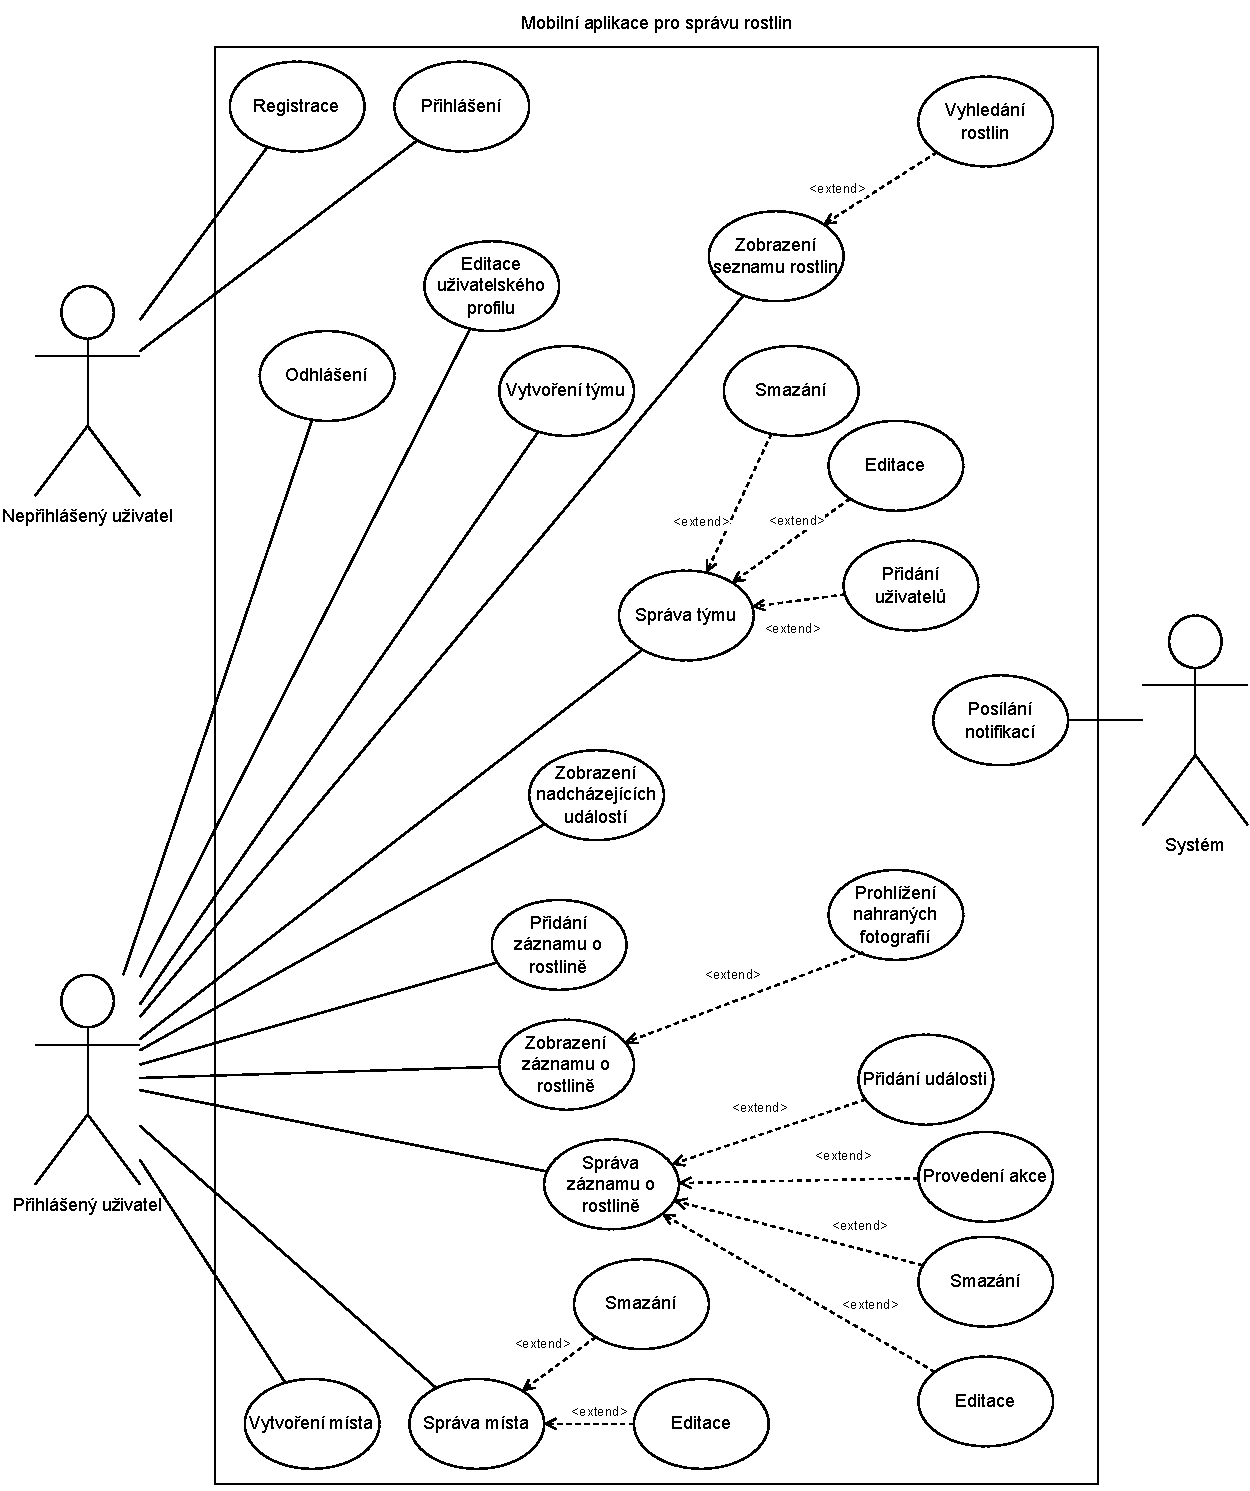
\includegraphics[width=1\linewidth]{images/use_case_diagram.pdf}
  	\caption{Diagram případů užití}
  	\label{dia:usecases}
\end{figure}

\subsection*{Případy užití}
\begin{description}
    
    \item[UC1 Registrace] Možnost vytvořit si svůj uživatelský účet, který bude využívat a vystupovat pod ním v~aplikaci. Tato možnost je dostupná, když v~aplikaci není přihlášený žádný uživatel. Registrace probíhá formou registračního formuláře, kde potenciální uživatel vyplní informace potřebné k~registraci.
    \begin{enumerate}
        \item Potenciální uživatel na úvodní obrazovce klikne na tlačítko/odkaz sloužící k~registraci uživatele.
        \item Aplikace uživateli zobrazí registrační formulář.
        \item Uživatel vyplní potřebné položky formuláře a odešle požadavek na registraci kliknutím na tlačítko.
        \item Systém ověří, zda zadané informace jsou v~pořádku. Pokud je tomu tak, uživatel je registrován a rovnou přihlášen. Naopak, pokud dojde k~nějaké chybě, uživatel je upozorněn.
    \end{enumerate}
    
    \item[UC2 Přihlášení] Přihlašovací proces uživatele, který už má vytvořený účet. Jednoduché vyplnění přihlašovacího formuláře s~jeho následným odesláním pro ověření.
    \begin{enumerate}
        \item Na úvodní obrazovce (pokud není v~aplikaci uživatel přihlášen) je uživateli zobrazen přihlašovací formulář.
        \item Uživatel vyplní přihlašovací formulář.
        \item Uživatel klikne na tlačítko k~odeslání požadavku na přihlášení.
        \item Zadané informace systém ověří a přihlásí uživatele do aplikace (uživatel existuje a heslo souhlasí) nebo v~případě chyby na ni upozorní.
    \end{enumerate}
    
    \item[UC3 Odhlášení] Uživatel očekává, že se může z~aplikace odhlásit. Odhlášení je možné jen pokud je uživatel již přihlášen.
    \begin{enumerate}
        \item Uživatel se nejdříve proklikne do nastavení.
        \item Následně klikne na odhlašovací tlačítko.
        \item Uživateli je zobrazeno potvrzovací okno, zda si přeje se opravdu odhlásit.
        \item Při potvrzení je uživatel odhlášen.
    \end{enumerate}
    
    \item[UC4 Editace a nastavení uživatele] Uživatel by měl mít možnost upravovat si svůj uživatelský účet (například změna hesla) a nastavit si funkcionality aplikace (např. zda bude dostávat notifikace).
    \begin{enumerate}
        \item Uživatel se nejdříve proklikne na obrazovku s~nastavením.
        \item Následně klikne na tlačítko, které slouží ke změně hesla.
        \item Uživateli je zobrazen formulář pro vyplnění nového hesla (součástí je stávající heslo pro potvrzení).
        \item Při potvrzení a splnění požadavků na nové heslo je uživateli změněno heslo.
    \end{enumerate}

    \item[UC5 Vytvoření týmu] Každý uživatel si může vytvořit tým, ve kterém bude společně s~dalšími uživateli sdílet informace o~pěstovaných rostlinách.
    \begin{enumerate}
        \item Uživatel vybere akci pro vytvoření týmu.
        \item Uživatel vyplní jméno týmu a potvrdí vytvoření.
    \end{enumerate}
    
    \item[UC6 Správa týmu] Členové týmů mají možnost spravovat daný tým. Uživatel očekává, že může měnit jméno týmu, přidávat a odebírat členy týmu, popřípadě tým smazat.
    \begin{enumerate}
        \item U~týmu uživatel vybere akci pro správu týmu.
        \item Následně je zobrazeno jméno, aktuální členové a tlačítko pro smazání týmu. Jméno může uživatel změnit a členy přidávat a odebírat.
    \end{enumerate}
    
    \item[UC7 Zobrazení seznamu rostlin] Seznam rostlin v~databázi aplikace, ve kterém lze vyhledávat.
    \begin{enumerate}
        \item Uživatel zobrazí obrazovku se seznamem rostlin.
        \item V~seznamu může uživatel scrollovat a vyhledávat pomocí jména.
        \item Kliknutím na některou rostlinu v~seznamu se může uživatel dostat na její detail.
    \end{enumerate}
    
    \item[UC8 Zobrazení detailu rostliny] Uživatel bude moci zobrazit detail o~konkrétní rostlině. Ten může zobrazit vybráním ze seznamu rostlin nebo proklikem z~konkrétního záznamu o~rostlině (týmové či osobní).
    \begin{enumerate}
        \item Uživatel zobrazí detail klikem na položku v~seznamu rostlin nebo tlačítkem na konkrétním záznamu o~rostlině.
        \item Uživateli je zobrazen detail o~rostlině, na kterém nalezne různé detaily ohledně dané rostliny.
    \end{enumerate}
    
    \item[UC9 Vytvoření místa] Uživatel bude moci vytvořit místo (místnost, část zahrady), do kterého pak lze přiřadit jednotlivé záznamy o~rostlinách.
    \begin{enumerate}
        \item Uživatel vyvolá akci k~vytvoření místa.
        \item Uživatel vyplní jednoduchý formulář k~vytvoření místa a následně ho potvrdí kliknutím na tlačítko.
    \end{enumerate}
    
    \item[UC10 Správa místa] Místo bude moci být editováno.
    \begin{enumerate}
        \item Uživatel vyvolá akci k~editaci místa.
        \item Je zobrazena editovací obrazovka místa.
        \item Uživatel vyplní požadované změny a potvrdí je tlačítkem.
    \end{enumerate}

    \item[UC11 Přidání záznamu o~rostlině] Uživatel bude moci přidat záznam o~konkrétní rostlině do svých nebo týmových rostlin. Toto lze provést z~detailu o~rostlině.
    \begin{enumerate}
        \item Uživatel se nachází na detailu rostliny a klikne na přidávací tlačítko.
        \item Uživateli se zobrazí obrazovka, která slouží k~vytvoření záznamu o~rostlině.
        \item Uživatel vyplní požadované informace k~vytvoření záznamu a klikne na tlačítko k~vytvoření daného záznamu.
        \item Daný záznam o~rostlině je systémem vytvořen a je rovnou uživateli zobrazen.
    \end{enumerate}
    
    \item[UC12 Zobrazení záznamu o~rostlině] Uživatel by měl být schopen zobrazit svůj/týmový záznam o~rostlině. V~záznamu by měl viděl budoucí události/akce, historii událostí/akcí, které byly kým u~daného záznamu provedeny, galerii fotografií daného záznamu.
    \begin{enumerate}
        \item Uživatel rozklikne daný záznam o~rostlině.
        \item Na příslušné obrazovce si může uživatel prohlížet detail záznamu.
    \end{enumerate}
    
    \item[UC13 Správa záznamu o~rostlině] Jednotlivé záznamy o~rostlinách by měly být možné spravovat uživatelem/i. Mělo by být možné zaznamenat provedení akce, změnit jméno a náhledovou fotografii, nahrát/odebrat fotografie.
    
    Provedení akce:
    \begin{enumerate}
        \item Uživatel klikne na tlačítko k~provedení akce.
        \item Uživatel vybere akci a potvrdí provedení.
        \item Akce je zaznamenána a přidána.
    \end{enumerate}

    \newpage
    Změna informací:
    \begin{enumerate}
        \item Uživatel rozklikne tlačítko pro editaci informací o~záznamu.
        \item Uživatel může vyplnit nové jméno záznamu, nahrát novou náhledovou fotografii a následně potvrdit změnu tlačítkem.
    \end{enumerate}
    
    Nahrání fotografie záznamu rostliny:
    \begin{enumerate}
        \item Uživatel klikne na záznamu o~rostlině na tlačítko k~přidání fotografie.
        \item Uživatel vyfotí nebo vybere fotografii k~nahrání a potvrdí ji.
    \end{enumerate}
    
    Odebrání fotografie v~galerii:
    \begin{enumerate}
        \item Uživatel zobrazí na záznamu o~rostlině galerii.
        \item Uživatel zobrazí fotografii, kterou chce odebrat.
        \item Uživatel klikne na tlačítko k~odebrání fotografie.
        \item Je zobrazeno potvrzovací okno, které uživatel potvrdí nebo zruší.
    \end{enumerate}
    
    \item[UC14 Zobrazení nadcházejících událostí] Zobrazení obrazovky, na které uživatel bude vidět jeho nadcházející události neboli akce jako chronologický seznam. Tato obrazovka bude tzv. domácí obrazovkou (první zobrazená obrazovka po otevření/přihlášení do aplikace).
    \begin{enumerate}
        \item Uživatel zobrazí obrazovku s~nadcházejícími událostmi, které jsou zobrazeny jako seznam.
        \item Uživatel může scrollovat událostmi a při kliku na událost se dostane k~vytvoření/potvrzení naplánované akce konkrétního záznamu o~rostlině.
    \end{enumerate}
    
    \item[UC15 Posílání notifikací] Systém bude uživatelům posílat notifikace. Jedná se o~připomínkové notifikace k~akcím a notifikace o~provedení akce uživatelem.
    
    Notifikace o~provedení akce:
    \begin{enumerate}
        \item Uživatel provede akci (například zalije rostlinu).
        \item Systém pošle notifikaci všem ostatním členům v~týmu (mají-li povolený tento druh notifikace), že uživatel provedl danou akci.
    \end{enumerate}
    
    Připomínková notifikace:
    \begin{enumerate}
        \item Uživatel má naplánovanou událost s~nastaveným připomínáním pomocí notifikací.
        \item V~daný okamžik je uživatel notifikován o~dané události.
    \end{enumerate}
    
\end{description}

Ověření, zda případy užití pokrývají funkční požadavky, je zobrazeno v~tabulce \ref{tab:fr-coverage}. Řádky jsou jednotlivé případy užití a sloupce jsou jednotlivé funkční požadavky. Písmeno \textit{X} v~buňkách zachycuje, kterému funkčnímu požadavku odpovídá který případ užití.

\begin{table}[H]
\begin{tabular}{|c|c|c|c|c|c|c|c|c|c|c|}
\hline
     & FR1 & FR2 & FR3 & FR4 & FR5 & FR6 & FR7 & FR8 & FR9 & FR10 \\ \hline
UC1  & X   &     &     &     &     &     &     &     &     &      \\ \hline
UC2  & X   &     &     &     &     &     &     &     &     &      \\ \hline
UC3  & X   &     &     &     &     &     &     &     &     &      \\ \hline
UC4  & X   &     &     &     &     &     &     &     &     &      \\ \hline
UC5  &     & X   &     &     &     &     &     &     &     &      \\ \hline
UC6  &     & X   &     &     &     &     &     &     &     &      \\ \hline
UC7  &     &     & X   &     &     &     &     &     &     &      \\ \hline
UC8  &     &     & X   &     &     &     &     &     &     &      \\ \hline
UC9  &     &     &     & X   &     &     &     &     &     &      \\ \hline
UC10 &     &     &     & X   &     &     &     &     &     &      \\ \hline
UC11 &     &     &     &     & X   &     &     &     &     &      \\ \hline
UC12 &     &     &     &     &     & X   &     &     &     &      \\ \hline
UC13 &     &     &     &     &     & X   & X   & X   &     &      \\ \hline
UC14 &     &     &     &     &     &     &     &     & X   &      \\ \hline
UC15 &     &     &     &     &     &     &     &     &     & X    \\ \hline
\end{tabular}
\caption{Tabulka pokrytí funkčních požadavků}
\label{tab:fr-coverage}
\end{table}

\section{Doménový model}
\begin{figure}
	\centering
	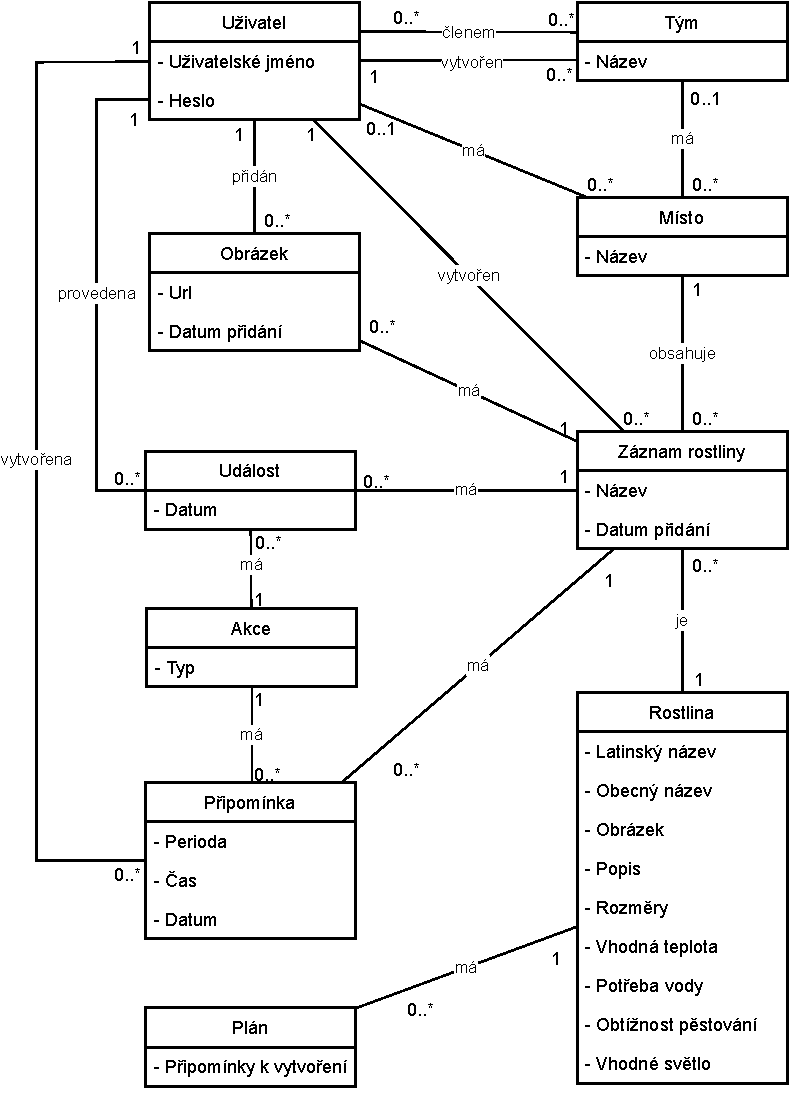
\includegraphics[width=1\linewidth]{images/domain-diagram.pdf}
  	\caption{Doménový model}
  	\label{dia:domain-model}
\end{figure}

Často může být obtížné si představit, jak bude problém strukturován a následně zpracován do technologické podoby. Proto se pro prvotní zachycení objektů a jejich vztahů mezi nimi se často používá doménový model. Ten je znázorněn zjednodušeným UML diagramem tříd. Jednotlivé entity jsou zobrazeny jako obdélníky, které mají uvnitř svůj název a důležité atributy. Entity jsou spojeny čárami, které znázorňují vztah mezi nimi. Spojující čáry mohou mít různé typy podle vztahu a na každém konci mají uvedenou multiplicitu. U~atributů se nespecifikuje jejich datový typ a celý doménový model by měl být platformě nezávislý. Na obrázku \ref{dia:domain-model} se nachází doménový model, který zachycuje doménu aplikace. Následuje popis jednotlivých entit v~samotném doménovém diagramu. \cite{domain-model-1, domain-model-2}

\begin{description}
    \item[Uživatel] Jedna z~hlavních entit celého systému. U~každého uživatele je nutné uchovávat jeho uživatelské jméno a heslo, respektive jeho hash. Noví uživatelé budou přidání po úspěšné registraci. Každý uživatel může vytvořit a být členem jednoho nebo více týmů. Dále k~němu patří žádné až více osobních míst a záznamů rostlin, které si vytvoří. Dále je také spojen s~žádnou nebo více konkrétními událostmi, které dokončil. Nakonec k~uživateli mohou patřit jednorázové a opakující se připomínky. Těch může mít více a nebo také žádnou.
    \item[Tým] Entita, která reprezentuje skupinu uživatelů. Je spojena s~konkrétním uživatelem, který daný tým vytvořil. Má jednoho až více členů (uživatelů) a žádné nebo více míst. Každý tým má také svůj název.
    \item[Místo] Místo je uživatelem vytvořená entita, která označuje, kde se rostlina nachází. Místo má svůj název a je spojen vždy buď s~jedním uživatelem nebo jedním týmem. Každé místo pak může obsahovat nula až více záznamů rostlin.
    \item[Záznam rostliny] Hlavní entita, jež reprezentuje konkrétní rostlinu (ne tedy o~jaký druh rostliny se jedná). Každý takový záznam má svůj název, obrázky a datum přidání. Záznam je spjat s~jedním konkrétním druhem rostliny (entita Rostlina), místem a uživatelem, který jej vytvořil. Dále je také spojen s~žádnou nebo více událostí, jednorázovou a opakující se připomínkou.
    \item[Rostlina] Entita popisující druh rostliny. K~atributům patří latinský a obecný název, její popis, obrázek. Dále také rozměry, teplotní rozpětí (krajní hodnoty intervalu -- minimum a maximum), ve kterém je rostlina schopna žít, kolik vody potřebuje, vhodné světlo a obtížnost pěstování.
    \item[Událost] Tato entita zachycuje jednotlivé události neboli také provedené akce. Má svůj typ/druh (zalití, přesazení atd.) a datum provedení. Je spojena s~uživatelem, který ji provedl a s~konkrétním záznamem o~rostlině.
    \item[Připomínka] Jedná se o~entitu, která popisuje aktivní připomínku. Ta obsahuje akci, kterou připomíná, a datum a čas. Dále může mít specifikovanou periodu, s~jakou se připomínka opakuje. Je spárovaná s~konkrétní rostlinou a konkrétním uživatelem, který ji vytvořil.
    \item[Akce] Jednoduchá entita, která znázorňuje akci (typ akce), kterou lze provést na rostlině. Může se vázat k~události nebo k~připomínce.
    \item[Obrázek] Jedná se o~entitu obsahující informaci o~obrázku konkrétního záznamu rostliny. Obsahuje URL obrázku, datum vytvoření a je spojena s~konkrétním záznamem rostliny a uživatelem, který obrázek vytvořil/pořídil.
    \item[Plán] Entita, která slouží pro definici jednotlivých plánů pro danou rostlinu. Každý plán má sadu připomínek na různé akce.
\end{description}

\section{Architektura a technologie}
V~této sekci je popsána architektura navrhované aplikace a také technologie, které budou použity pro vývoj a implementaci. Popsána je architektura jako celek a poté jednotlivě každá část aplikace, neboli také vrstva (databáze, serverová část, klientská část).

\subsection{Třívrstvá architektura}
Třívrstvá architektura (anglicky \textit{Three-Tier Architecture}) je v~současnosti jedna z~nejpoužívanějších architektur ve vývoji softwaru, která vychází z~klient-server architektury. Klíčovou vlastností je rozdělení aplikace na tři části (vrstvy), přičemž tyto části nejsou na sobě závislé. Každá část běží odděleně a má přístup jen ke zdrojům, které opravdu potřebuje. Díky nezávislosti může vývoj jednotlivých částí aplikace probíhat zvlášť. Na obrázku \ref{img:three-tier-architecture} se nachází zjednodušený diagram, který tuto architekturu popisuje. \cite{three-tier-architecture-1, three-tier-architecture-2}

\begin{description}
    \item[Prezentační vrstva] Vrstva, se kterou se setkává uživatel. Jedná se o~klientské aplikace, které zaznamenávají uživatelské vstupy a na jejich základě zobrazují a prezentují data. Tyto aplikace jsou závislé na platformě, typicky se dnes vyvíjejí webové a mobilní aplikace. Komunikuje s~aplikační vrstvou (serverem), ale zároveň nemá přímý přístup k~datům v~databázi.
    \item[Aplikační vrstva] Tato vrstva, také nazývaná jako logická, prostřední, či byznysová vrstva, se stará o~hlavní funkce aplikace. Zde probíhají hlavní výpočty a logika nad daty, které napřímo získává a ukládá do databáze. Nabízí rozhraní pro komunikaci s~klientskými aplikacemi (prezentační vrstvou).
    \item[Datová vrstva] Entity starající se o~ukládání, řízení, audit a poskytování dat.
\end{description}

Tato architektura bude použita při vývoji aplikace. Prezentační vrstva bude obsahovat klientskou aplikaci pro iOS. Ta bude komunikovat s~aplikační vrstvou pomocí REST API. Data poté budou ukládána v~databázi, která patří do datové vrstvy.

\begin{figure}
	\centering
	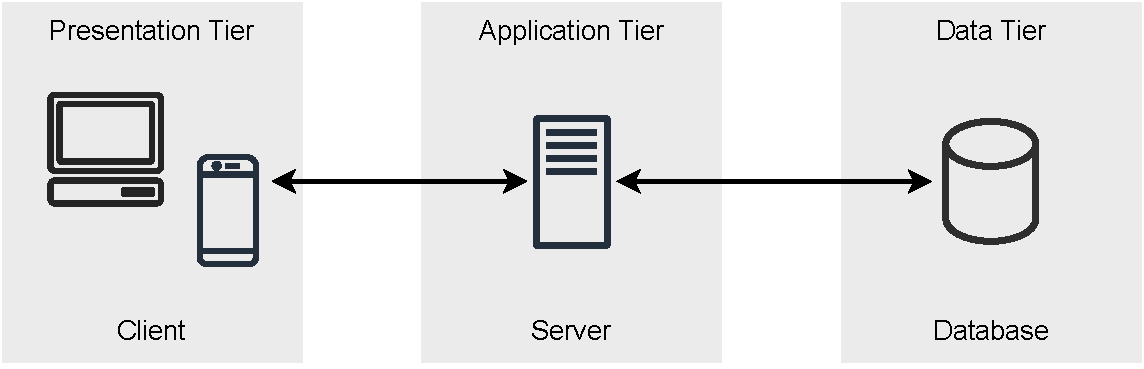
\includegraphics[width=1\linewidth]{images/three-tier-architecture.pdf}
  	\caption{Třívrstvá architektura}
  	\label{img:three-tier-architecture}
\end{figure}

\subsection{Datová vrstva}
Výběr databázového systému, který bude použit k~uložení perzistentních dat, je poměrně přímočarý. Nejdříve je nutné zvolit o~jaký typ databáze by se mělo jednat. Vzhledem k~datům, které se budou ukládat a zároveň kvůli jejich množství (nejedná se o~žádná enormní data), je vhodné použít standardní relační databázi. V~tomto segmentu se nachází 4 nejpopulárnější možnosti, jimiž jsou relační databázové systémy Oracle, Microsoft SQL Server, MySQL, PostgreSQL \cite{database-layer}. První dva zmíněné systémy nejsou zástupci otevřeného softwaru (open source), zatímco zbytek ano. Zároveň vzhledem k~použití ORM Prisma (viz \ref{doc:prisma}) odpadá Oracle databáze, jelikož není podporována. Dále už je volba spíše o~osobní preferenci a zkušenosti. Ačkoliv je vnitřek každého systému odlišný, používají dotazovací jazyk SQL a pracuje se s~nimi obdobně. S~ohledem na budoucí nasazení aplikace (na cloudovou platformu Heroku) tak konečná volba padla na PostgreSQL. Zároveň ovšem není problém kdykoliv databázový systém v~případě potřeby změnit, a to kvůli využití nástroje Prisma.

\subsubsection{PostgreSQL}
PostgreSQL je pokročilá open source relační databáze, která podporuje dotazování v~jazyce SQL (relační) i JSON (nerelační). Jedná se o~vysoce stabilní systém pro správu databází, za kterým stojí více než 20 let komunitního vývoje, který přispěl k~jeho vysoké úrovni odolnosti, integrity a správnosti. PostgreSQL se používá jako primární datové úložiště nebo datový sklad pro mnoho webových, mobilních, geoprostorových a analytických aplikací. Nejnovější hlavní verzí v~době psaní této práce je PostgreSQL 14. PostgreSQL má bohatou historii podpory pokročilých datových typů a vysokou úroveň optimalizace výkonu. Dále také umožňuje běh uložených procedur napsaných v~různých programovacích jazycích (Python, Perl, C). \cite{postgresql-1, postgresql-2}

\subsection{Aplikační vrstva}
Technologií, které lze v~dnešní době použít k~implementaci serverové části aplikace, je nepřeberné množství. Vývojáři si mohou vybrat z~různých frameworků a programovacích jazyků s~nimi spjatých. Vhodné je, vzhledem k~nefunkčnímu požadavku vytvořit REST API rozhraní pro komunikaci, vybrat vhodný framework, který tvorbu REST API umožňuje a co nejvíce usnadňuje. Protože se nejedná a aplikaci výpočetně náročnou, není potřeba se orientovat na takové technologie, které se na rychlost a výkonnost přímo specializují. Důležité je se spíše zaměřit na framework, který umožňuje psát přehledný a znovupoužitelný kód. Nakonec volba padla na framework \textit{NestJS} \cite{nestjs}, který používá prostředí \textit{Node.js}. Dalším nástrojem, který byla zvolen, je \textit{Prisma}, což je technologie pro objektově relační mapování (ORM). \textit{Prisma} usnadňuje práci s~daty a dokáže spolu s~\textit{NestJS} výborně spolupracovat, neboť obě dvě technologie si zakládají především na typové bezpečnosti (použití programovacího jazyka \textit{TypeScript}).

\subsubsection{NestJS}
\textit{NestJS} je progresivní framework, pomocí kterého lze vytvářet aplikace na straně serveru. Autorem tohoto frameworku je polský vývojář Kamil Myśliwiec. \textit{NestJS} samotný staví na frameworcích \textit{Express} nebo \textit{Fastify}, a přidává modulární organizaci a širokou škálu dalších knihoven. Jedná se o~open-source software, používá programovací jazyk \textit{TypeScript} a struktura kódu výrazně připomíná framework \textit{Angular}. Podporuje tvorbu aplikačního rozhraní REST a GraphQL. Klíčové vlastnosti, o~které \textit{NestJS} usiluje, jsou efektivita, spolehlivost a škálovatelnost aplikací. Velkou výhodou je velmi přehledná a propracovaná dokumentace a živá komunita. \cite{nestjs, nestjs-1, nestjs-2}

Hlavními komponentami NestJS aplikace jsou:
\begin{description}
    \item[Controller] Controllery jsou zodpovědné za zpracování příchozích požadavků a vracení odpovědí klientovi.
    \item[Provider] Slouží k~zapouzdření a abstrakci logiky jiných tříd. Lze je vkládat do jiných tříd pomocí dependency injection (vkládání závislostí).
    \item[Module] Moduly slouží ke sdružování souvisejících funkcí, controllerů a providerů.
\end{description}


\subsubsection{Prisma}
\label{doc:prisma}
Prisma je poměrně nová open-source knihovna pro Node.js, která slouží k~objektově relačnímu mapování (ORM). Objektově relační mapování je technika, která propojuje relační databázi a objektově orientovaným programovacím jazykem pomocí automatické konverze dat. Umožňuje přistupovat k~databázi prostřednictvím metod a objektů daného programovacího jazyka (TypeScript nebo JavaScript v~případě knihovny Prisma), aniž by bylo nutné psát dotaz v~samotném databázovém jazyce. Prisma se skládá ze tří částí.
\begin{description}
    \item[Prisma Client] Automaticky generovaný a typově bezpečný databázový klient.
    \item[Prisma Migrate] Výkonný nástroj pro migraci databázových schémat. K~popisu databázového schématu používá deklarativní syntaxi. Také ukládá celou historii migrací a umožňuje snadno se vracet a znovu opakovat migrace.
    \item[Prisma Studio] Nástroj pro zobrazení a editaci dat v~prohlížeči. Nabízí moderní UI a snaží se být jednoduchý a přehledný.
\end{description}
Hlavním způsobem, jak interagovat s~projektem Prisma z~příkazového řádku je použití Prisma CLI (Command Line Interface). Tak lze vytvářet nové prostředky projektu, generovat klienta a analyzovat stávající struktury databáze pomocí introspekce a automaticky vytvářet modely. Knihovna Prisma je přímo připravená pro framework NestJS a výborně spolupracuje s~jeho modulární architekturou. \cite{prisma, prisma-1}

\subsection{Prezentační vrstva}
V~současnosti se vývoj mobilních aplikací dělí na nativní a multiplatformní. Nativní mobilní aplikace jsou vytvářeny s~nástroji specifickými pro danou platformu. Vzhledem k~tomu tak dokážou poskytnout skvělý pocit z~používání, protože jsou výkonnější, optimalizované a také používají na míru šité vizuální prvky pro danou platformu. Nevýhodou jsou vyšší náklady (lidské i peněžní) na vývoj, neboť je potřeba vytvořit separátní aplikace pro každou platformu. Proto vznikly frameworky, se kterými lze vytvářet aplikace na více platforem najednou. Mezi tyto frameworky se řadí například \textit{React Native} nebo \textit{Flutter}. Výhodou je jediná \textit{codebase}, což šetří prostředky a urychluje vývoj. Aplikace ale nemusí být optimalizované a mohou vypadat a chovat se lehce jinak na každé platformě. Z~důvodu lepší optimalizace/výkonu, použití nativních vizuálních prvků a protože není potřeba implementovat aplikaci na jiné platformy, jsem se rozhodl pro nativní vývoj. \cite{native-vs-multiplatform}

\subsubsection{SwiftUI}
Tradičním a historickým způsobem, jakým lze psát nativní aplikace pro iOS, je použití frameworku UIKit. Ten je podporován pro jazyky Objective C a Swift a kód je psán imperativním způsobem. Stále je hojně využívaný, neboť je odladěný a má za sebou mnoho let vývoje. V~roce 2019 Apple ovšem představil nový framework s~názvem SwiftUI. Ten nabízí deklarativní psaní kódu a reaktivní přístup. Nějakou dobu nebylo stále vhodné tento framework používat, protože byl dosti problémový a pro reálné aplikace se nedal téměř použít. Po třech letech si ale dovolím tvrdit, že se dostal do stavu, kdy se stal použitelným a v~mnoha ohledech dokáže předčit samotný UIKit. A~pokud by se ovšem vyskytl nějaký problém s~implementací určité věci, lze ji vytvořit v~UIKitu a vložit do SwiftUI. \cite{swiftui}

Nejnovější verze operačního systému iOS je v~době psaní této práce verze 16. Na tuto verzi zároveň bude implementována výsledná aplikace. Vzhledem k~faktu, že Apple poskytuje aktualizace poměrně starým zařízením (5 let staré) a zároveň mezi uživateli je tendence udržovat systém aktuální, omezení se pouze na nejnovější verzi by nemělo být kritické. Použití nejnovější verze zároveň znamená, že lze použít nově přidané prvky a nástroje. Statistiky obchodu s~aplikacemi App Store \cite{app-store-stats} navíc udávají, že zhruba 8 měsíců po vydání nové verze bývá zvykem, že je právě tato nejnovější verze nainstalována na 82 procentech zařízení.

Dále Apple pomalu upouští od vývoje frameworku UIKit a soustředí si na SwiftUI, který by měl být primárním frameworkem pro tvorbu nativních aplikací pro mobilní zařízení od společnosti Apple. I~proto byl také framework SwiftUI zvolen pro následnou implementaci klientské části aplikace.

\subsubsection{MVVM}
Vybranou architekturou pro vývoj iOS aplikace je architektura MVVM (Model View ViewModel). Vychází z~architektury MVC (Model View Controller) a zároveň se jí velmi podobá. Hlavním důvodem, proč se používají tyto architektury (a spoustu dalších), je oddělení částí aplikace pro lepší přehlednost a na základě toho i rozšiřitelnost kódu. V~případě MVVM se jedná o~rozdělení na tři části -- Model, View, ViewModel (viz \ref{img:mvvm}). Model obsahuje data, se kterými aplikace pracuje. View reprezentuje veškeré prvky uživatelského rozhraní, čili to, jak aplikace vypadá. Uprostřed je ViewModel, který slouží jako prostředník mezi View a Modelem. Ten provádí veškerou dodatečnou logiku a drží stav aplikace. Typicky je View spojen s~ViewModelem pomocí konstrukce zvané \textit{binding}. View pak dokáže reagovat na změny v~přidruženém ViewModelu a překreslovat tak uživatelské rozhraní. \cite{mvvm-1}

SwiftUI přímo nestaví na žádné architektuře, nicméně architektura MVVM se výborně hodí pro použití. Ve SwiftUI existují Views, ve kterých se pomocí deklarativního kódu popisují prvky na obrazovce. Samotné View pak drží referenci (a je spojen pomocí \textit{binding} konstrukce) na přidružený ViewModel. Všechny uživatelské vstupy/akce jsou delegovány na ViewModel, kde probíhá samotná logika a v~případě potřeby se mění stav aplikace, na kterou reaktivně reaguje View (překreslením změněných prvků). Modely jsou pak jen jednoduché třídy, které uchovávají a zapouzdřují data. S~těmi pracuje výhradně ViewModel. \cite{mvvm-2}

\begin{figure}
	\centering
	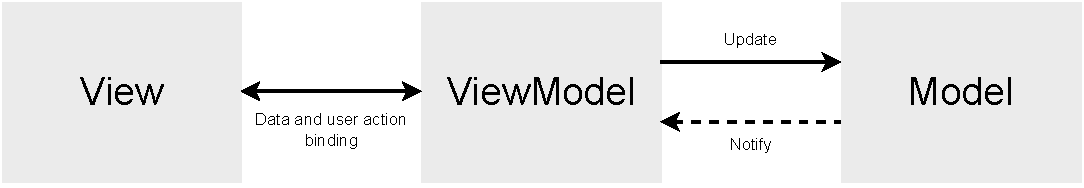
\includegraphics[width=1\linewidth]{images/mvvm.pdf}
  	\caption{Architektura MVVM (Model View ViewModel)}
  	\label{img:mvvm}
\end{figure}

\subsection{Autentizace}
Protože samotné rozhraní bude na internetu veřejně dostupné, je potřeba zajistit zabezpečení, aby kdokoliv nemohl přistupovat k~datům. Prvním způsobem, jak zabezpečit přístup je tzv. \textit{Basic} autentizace. Ta spočívá v~poslání uživatelského jména a hesla zakódovaného pomocí Base64 v~hlavičce požadavku. Tento způsob je velmi jednoduchý, ale není doporučován z~hlediska bezpečnosti. Dále se používá autentizace pomocí API klíče. V~hlavičce nebo přímo v~URL požadavku je posílán řetězec znaků (klíč) vygenerovaný serverem. Dalším způsobem je \textit{Bearer} autentizace, při které se posílá v~hlavičce tzv. access token, který jasně identifikuje tázající se entitu. Tento token vydává sám server a může mít definovanou expirační dobu. Proto se také spolu s~tímto tokenem vystavuje refresh token, pomocí kterého lze dostat od serveru nový platný access token. Pokud aplikace používá data aplikace třetích stran, využívá se autentizace pojmenovaná \textit{OAuth 2.0}, jejíž koncept je podobný \textit{Bearer} autentizaci, dochází také k~vystavování a ověřování tokenů, ale o~toto se nestará samotná aplikace, ale právě třetí strana. \cite{rest-auth-1, rest-auth-2}

\begin{figure}
	\centering
	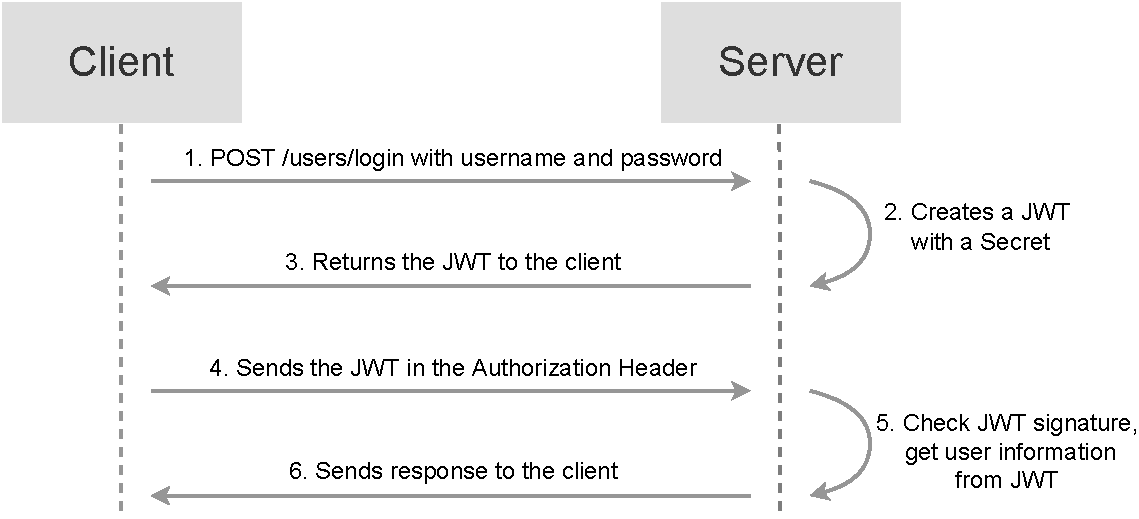
\includegraphics[width=1\linewidth]{images/jwt-flow.pdf}
  	\caption{Interakce mezi klientem a serverem při použití JWT}
  	\label{img:jwt-flow}
\end{figure}

Pro aplikaci byla vybrána \textit{Bearer} autentizace, přičemž samotný token bude řešen jako JWT (JSON Web Token) \cite{jwt}. Token bude tedy zakódovaná (Base64) trojice hlavička-data-podpis (header-payload-signature). V~hlavičce se nachází typ a hashovací funkce, v~datech vydavatel, subjekt, čas vypršení a další libovolná data. Podpis je poté vytvořen z~hlavičky a dat pomocí specifikované hashovací funkce a tajného klíče. Na obrázku \ref{img:jwt-flow} je popsána interakce klienta a serveru při použití JWT tokenu.

\section{Návrh API rozhraní}
Z~nefunkčních požadavků vyplývá použití architektonického vzoru REST pro návrh API. REST, z~anglického \textit{Representational State Transfer}, popisuje pravidla, dle kterých se mají aplikační rozhraní vytvářet. Komunikace poté probíhá tím způsobem, že entita, která chce získat/modifikovat data, pošle požadavek (request) na konkrétní endpoint pomocí HTTP protokolu a následně dostane zpět odpověď. Každý požadavek obsahuje informaci o~použité HTTP metodě, v~případě dodržení pravidel REST se jedná typicky o~metody GET (získání), POST (vytvoření), PUT (modifikace celku), PATCH (modifikace části), DELETE (smazání). Dále také požadavek obsahuje samotný endpoint, HTTP hlavičky a tělo (body), ve kterém jsou obsaženy samotná data. Data lze poslat v~různých formátech (formát je specifikován v~hlavičce požadavku), mezi nejpoužívanější formáty patří JSON, XML nebo pouze text (plain text). \cite{rest-1, rest-2}

Server by měl podporovat veškeré nutné operace, které bude využívat klientská aplikace (v~tomto případě mobilní aplikace). Jedná se tedy o~autentizaci, CRUD operace nad jednotlivými entitami a specifické operace (například nastavení plánu).

\section{Uživatelské rozhraní}
Uživatelské rozhraní (zkratka UI) je ve zkratce souhrn všech grafických prvků a jejich uspořádání, které slouží pro komunikaci mezi uživatelem a aplikací či webem (obecně se strojem). S~UI úzce souvisí termín UX. UX je zkratka pro uživatelskou zkušenost (User Experience), jde o~propojení a interakci grafických prvků, tak aby průchod aplikací byl snadný a intuitivní a aby dosažení požadovaného výsledku vyžadovalo minimální úsilí ze strany uživatele. Dobré UI a UX je stejně tak klíčové, jako samotné funkce dané aplikace. Ty můžou být prvotřídní, ale pokud je aplikace zpracována vizuálně špatně a neintuitivně, uživatel si může vytvořit odpor k~jejímu používání. Tento fakt je ještě více umocněn u~aplikací, které uživatelé používají primárně dobrovolně (nepoužívají je pro práci, ale ve volném čase). \cite{what-is-ui}

\subsection{Prototypování}
Tímto termínem je myšlen proces, při kterém jednotlivec či tým designérů realizují svoje nápady do papírové či digitální podoby ve formě tzv. prototypu. Hlavním cílem jeho tvorby je vyzkoušet a otestovat návrh uživatelského rozhraní před vytvořením skutečného produktu, neboť přepracovávat hotový produkt je mnohem nákladnější než jeho prototyp. Pro tvorbu prototypu lze využít různé nástroje a software nebo také pouze tužku a papír. Jednotlivé prototypy mají podle potřeby různý stupeň přesnosti (fidelity) a dělí se na Lo-Fi a Hi-Fi. Vytvořené prototypy slouží k~prezentaci a konzultaci s~klienty a jako podklad pro vývojáře. \cite{prototyping-101}

\subsubsection{Lo-Fi prototyp}
Jedná se o~prototypy s~nízkou přesností či věrností. Jde o~prvotní pohled na budoucí aplikaci a důraz je kladen zejména na rozmístění, typ a velikost grafických prvků. Neřeší se barvy, nevkládají se reálné hodnoty, texty ani obrázky. Lo-Fi prototyp lze vytvořit jen za pomocí papíru a tužky, ale také specializovanými nástroji. Výhodou tohoto prototypu je zejména rychlost zhotovení a jeho nízká cena. Samotný prototyp se může následně dotvořit (nebo může sloužit jako podklad) v~Hi-Fi prototyp. Příklad Lo-Fi prototypu je znázorněn na obrázku \ref{img:lo-fi-prototyp}. \cite{prototypes-difference}

\begin{figure}
	\centering
	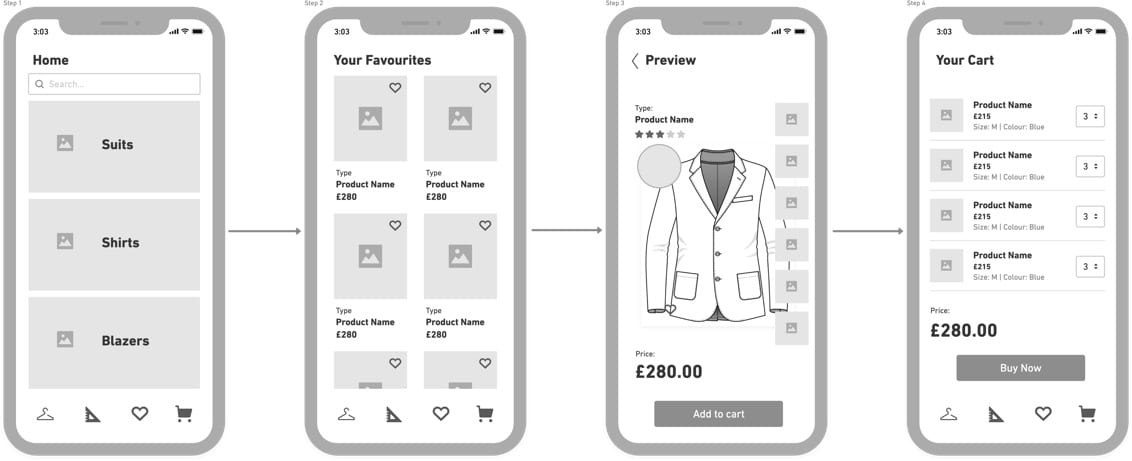
\includegraphics[width=1\linewidth]{images/lo-fi-prototype.jpg}
  	\caption{Lo-Fi prototyp \cite{prototype-examples}}
  	\label{img:lo-fi-prototyp}
\end{figure}

\subsubsection{Hi-Fi prototyp}
Takový prototyp by měl znázorňovat téměř finální vzhled výsledného produktu (nemusí však být funkční). Zachycuje konkrétní vzhled a barvu prvků, propojení jednotlivých obrazovek, včetně animací a přechodů. Pro jeho tvorbu lze využít mnoha nástrojů nebo prototyp přímo implementovat pro danou platformu. Tento prototyp je na tvorbu časově mnohem náročnější a nákladnější a někdy se lze bez něj obejít. Výhodou je na druhou stranu ovšem zobrazení téměř finální podoby, kterou klient nakonec dostane. Na obrázku \ref{img:hi-fi-prototyp} je zobrazen takovýto prototyp. \cite{prototypes-difference}

\begin{figure}
	\centering
	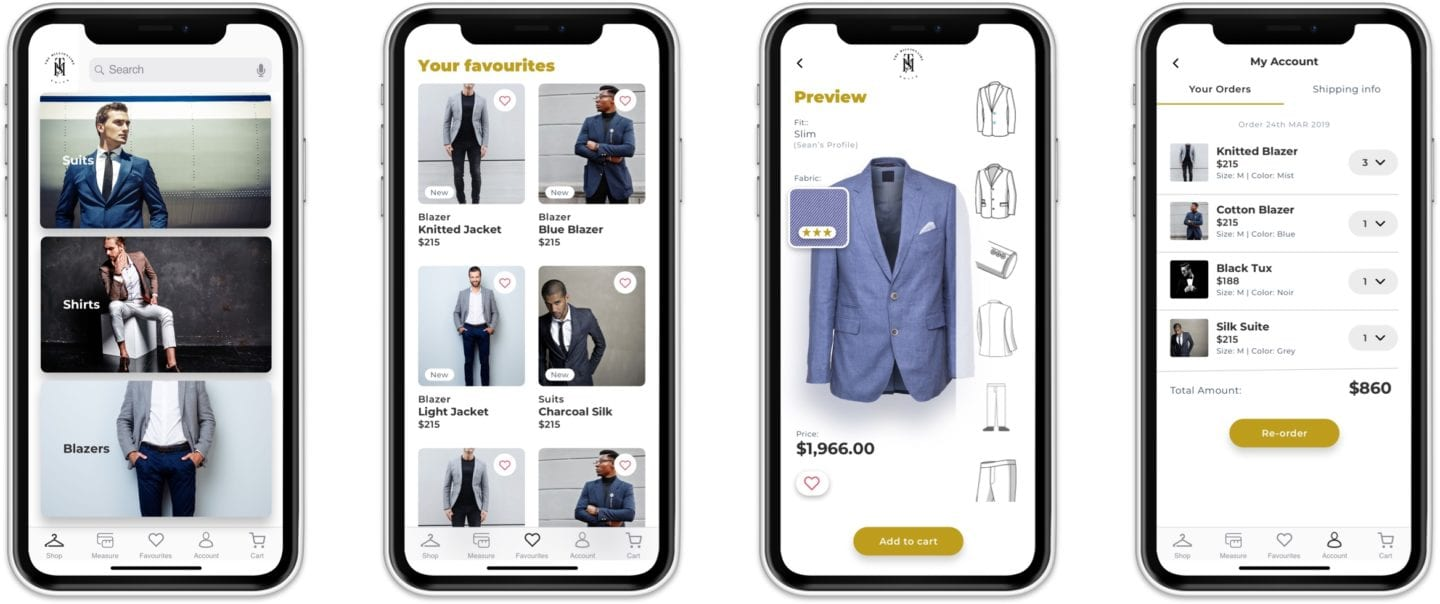
\includegraphics[width=1\linewidth]{images/hi-fi-prototype.jpg}
  	\caption{Hi-Fi prototyp \cite{prototype-examples}}
  	\label{img:hi-fi-prototyp}
\end{figure}

\subsubsection{Volba druhu prototypu}
V~rámci této závěrečné práce byl zvolen a zhotoven prototyp, který spadá spíše do kategorie Hi-Fi prototypů, ale zároveň se nejedná úplně o~jeho plnohodnotného zástupce. Vzhledem k~absenci klientské strany, nebylo potřeba dbát tolik na tvorbu dokonalého prototypu. Stačilo sestavit a poskládat grafické prvky do uceleného celku, který bude sloužit jako reference k~implementaci. K~tomu by postačila tužka a papír nebo nějaký jednoduchý nástroj. Protože jsem ale zvolil nástroj Figma, který je popsán v~následující sekci, naskytla se možnost velmi jednoduše vytvořit i klikatelný prototyp. Výsledný prototyp (popsán níže) jsou tedy vzájemně propojené (klikatelné) obrazovky, které obsahují nebarevný nástin grafických prvků.

\subsection{Figma}
Figma je webová aplikace pro tvorbu/editaci grafiky a návrh uživatelského rozhraní. Lze s~ní vytvářet nejrůznější grafické počiny od vytváření drátěných modelů webových stránek, přes navrhování rozhraní mobilních aplikací, jejich prototypování až po tvorbu reklamních bannerů. Aplikace funguje přímo v~prohlížeči a pro její používání je potřeba mít uživatelský účet. Výhodou toho je, že uživatel má přístup ke svým projektům (ty jsou uloženy v~cloudu) z~libovolného počítače nebo platformy. Velkou výhodou je také týmová kolaborace v~reálném čase na stejném projektu a dále také veliká komunita, kdy každý může přispět sdílením svých projektů (jako inspirace pro ostatní) nebo vytvořením šablony či pluginu. Figma je dostupná komukoli zadarmo s~několika omezeními (maximálně 3 projekty, omezený přístup k~historii verzí, omezené zabezpečení), které pro nenáročnou práci stačí. Náročnější uživatelé si poté mohou zaplatit za některé z~placených plánů. Na obrázku \ref{img:figma-screenshot} se nachází ukázka rozhraní aplikace Figma (na demo projektu, který se věnuje prototypování). \cite{figma}

\begin{figure}
	\centering
	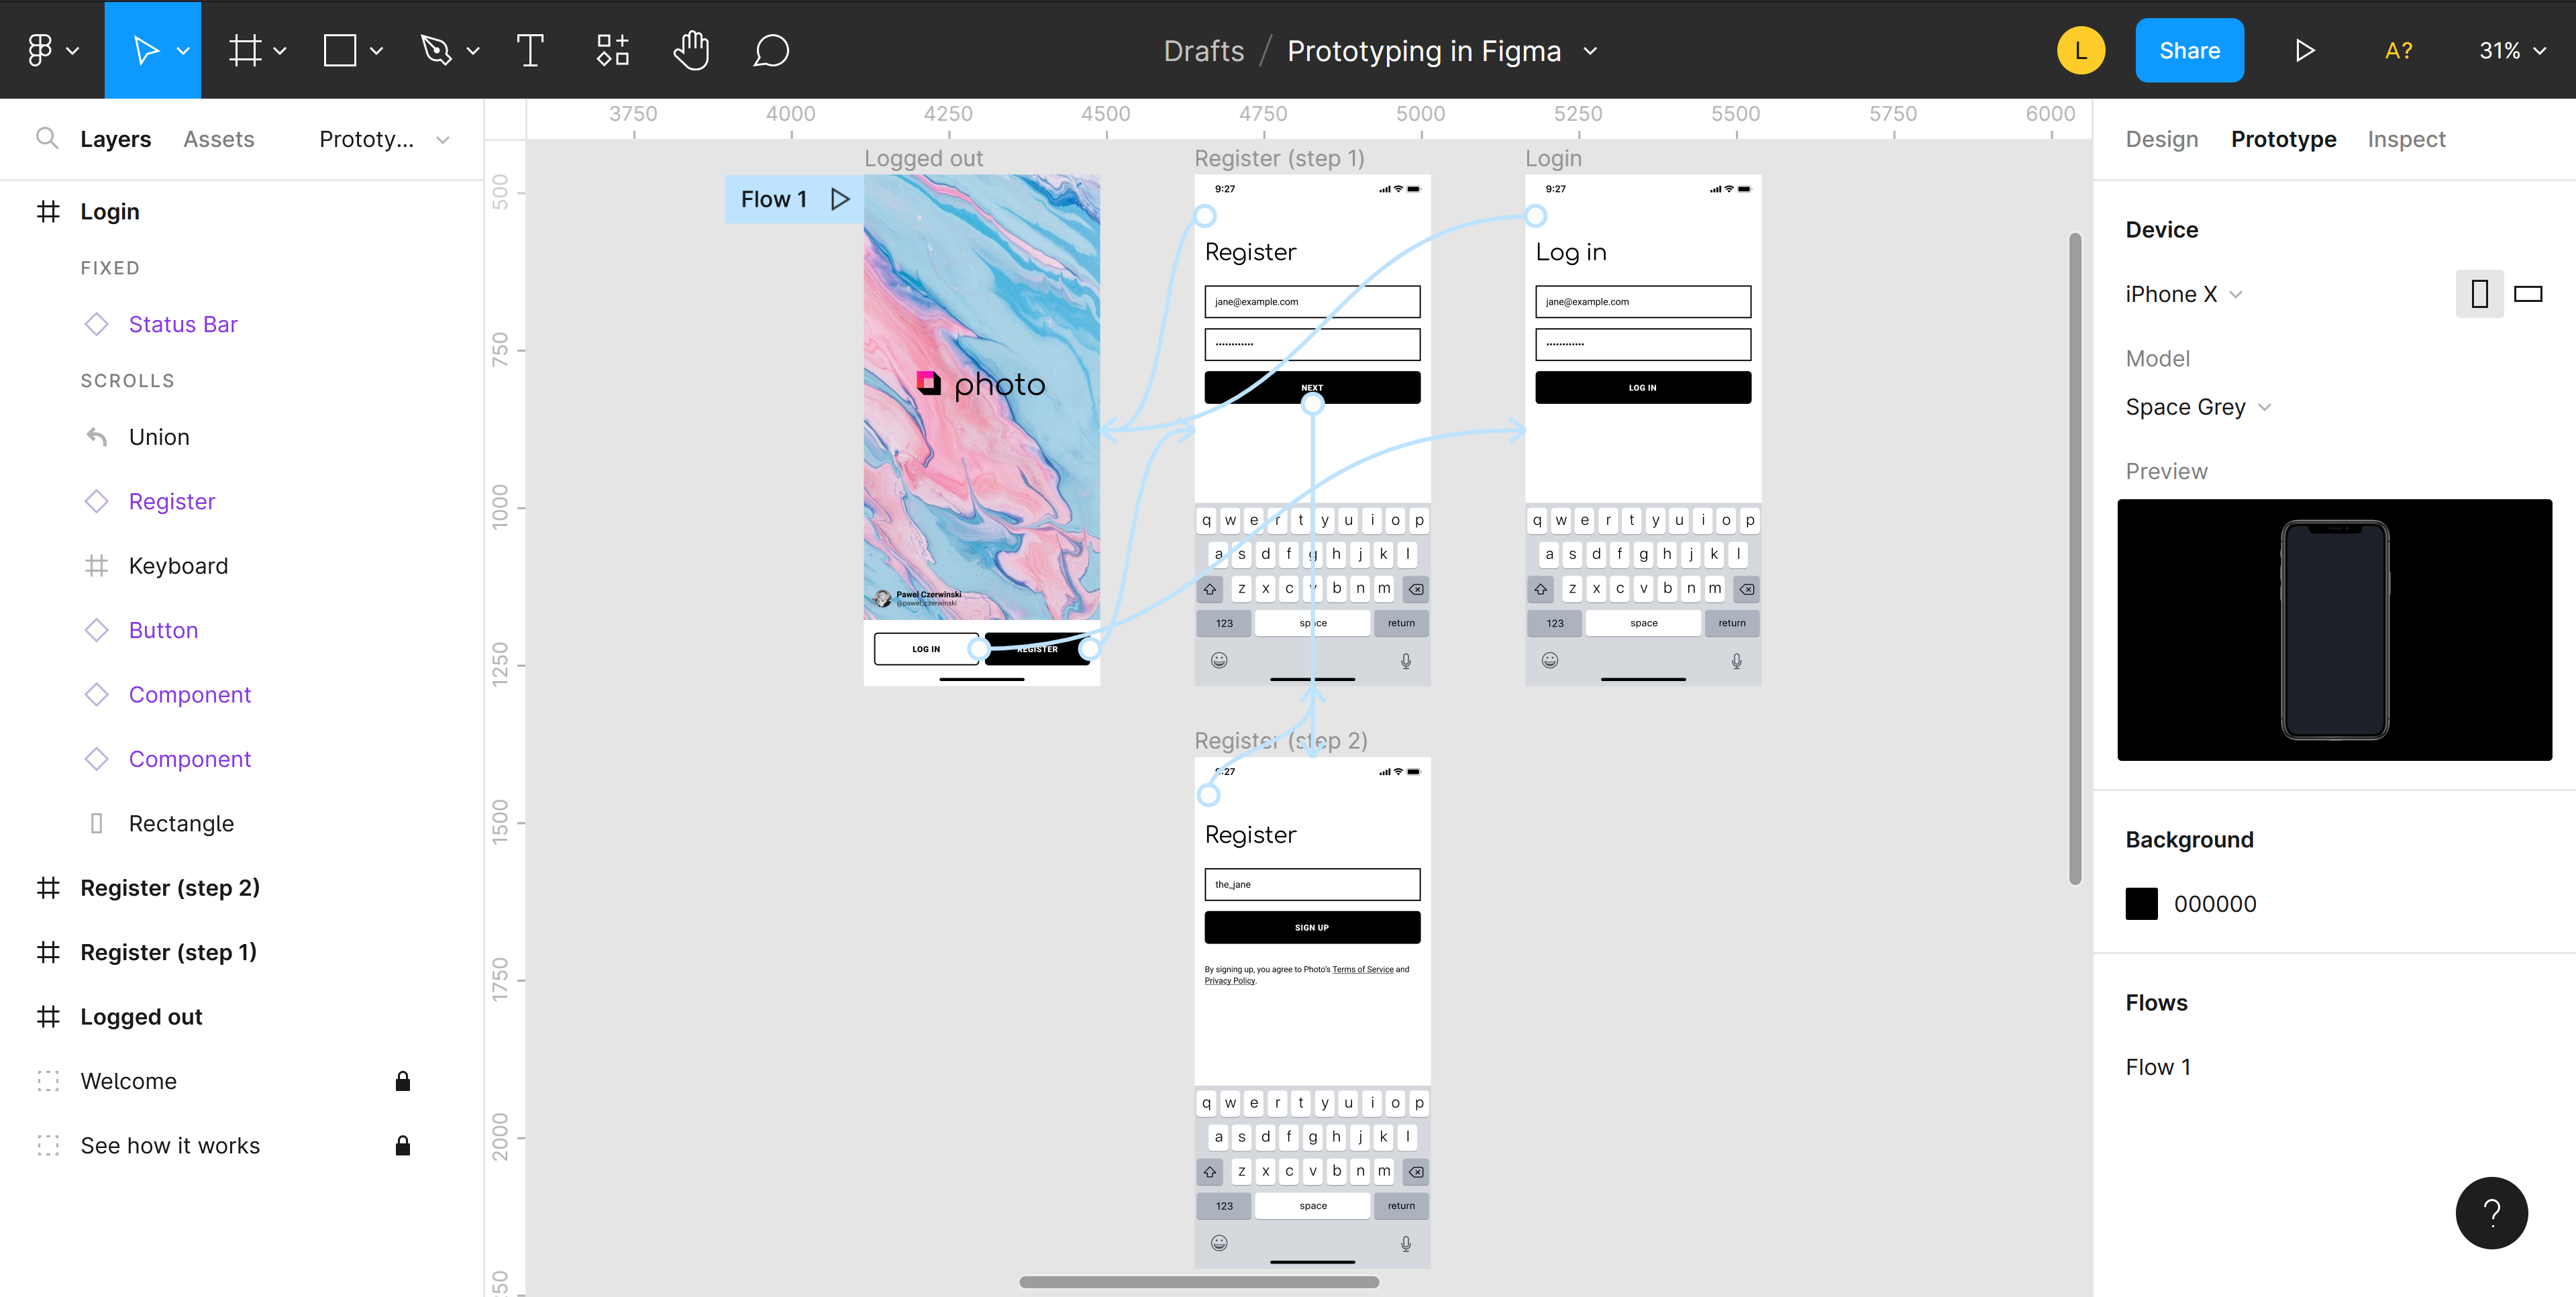
\includegraphics[width=1\linewidth]{images/figma-screenshot.png}
  	\caption{Screenshot z~nástroje Figma}
  	\label{img:figma-screenshot}
\end{figure}

\subsection{Vytvořený prototyp}
Prototyp byl vytvořen, jak již bylo zmíněno v~aplikaci Figma. Zjednodušený diagram klíčových obrazovek a jejich přechodů je vyobrazen na obrázku \ref{img:view-flow}. Nejsou na něm zachyceny veškeré přechody (například navigace zpět) a některé obrazovky jsou spojeny do jedné. Klikatelný prototyp je dostupný na \cite{figma-prototyp}, popřípadě všechny samotné obrazovky (včetně kontextových nabídek) se nachází na přiloženém médiu ve formátu PDF. Ukázku několika obrazovek a kontextových nabídek lze nalézt v~obrázku \ref{img:prototype-showcase}.

První obrazovkou, se kterou se nový uživatel setká, je přihlašovací obrazovka (Sign In). Na té se může přihlásit a dostat se do aplikace (pokud již má vytvořený účet), nebo se překliknout na registrační obrazovku (Sign Up). Pokud se úspěšně registruje, zobrazí se mu Onboarding, což je krátké seznámení s~klíčovými funkcemi aplikace. Po jeho dokončení se dostane do samotné aplikace.

Samotná aplikace se skládá ze 4 hlavních obrazovek, respektive oddělených sekcí. Těmi jsou obrazovky \textit{Tasks}, \textit{My Plants}, \textit{Search Plants} a \textit{Profile}. Mezi těmito sekcemi lze přepínat pomocí dolního panelu, který je známý pod anglickým spojením \textit{Bottom Tab Bar}. Tento panel patří obecně mezi nejoblíbenější navigační prvky mobilních zařízení (iOS i Android) a nachází se ve většině nejpopulárnějších aplikací. Výhodou je jeho poloha, která umožňuje jednoduché ovládání pomocí palce. Ačkoliv se jedná o~velmi jednoduchý grafický prvek, je potřeba si dát záležet a nepodcenit jeho návrh. Dolní panel by měl ideálně obsahovat 3 až 5 tlačítek, které neprovádějí akce, ale pouze přepínají mezi oddělenými obrazovkami/sekcemi. Samotná tlačítka by měla mít výstižnou ikonku a pod ní se může nacházet popisek (nutný, pokud není nebo neexistuje dosti reprezentativní ikonka). Také by panel neměl být posunovací a neměl by zbytečně mást uživatele složitými animacemi. \cite{bottom-tab-bar}

První obrazovkou je obrazovka \textit{Tasks}, na které se nachází seznam nadcházejících úkolů, respektive budoucích událostí, které budou v~daný čas připomenuty. V~dolním panelu se tato obrazovka nachází úplně nalevo a je reprezentována ikonkou papírového seznamu úkolů. Cílem je zobrazit uživateli jednoduchý přehled úkolů a umožnit mu jednoduše jednotlivé úkoly dokončit.

Obrazovka \textit{My Plants}, kterou reprezentuje ikonka dvou lístků, poskytuje ucelený pohled na uživatelovy rostliny. Na této obrazovce se vpravo nahoře nachází tlačítko pro vytvoření týmu, místa či přidání záznamu rostliny. Níže se pod sebou nachází horizontálně posuvný seznam míst, které přísluší jednotlivým týmům. Do detailu týmu se uživatel dostane kliknutím na jméno týmu, odkud poté může spravovat daný tým. Místo je zobrazeno zaobleným čtvercem, na kterém se nachází až 4 záznamy rostlin, které se nachází v~daném místě (jsou k~němu přiřazeny). V~samotném místě jich ale ovšem může být více než 4, jedná se pouze o~náhled. Po posledním místě se vždy nachází tlačítko (zaoblený čtverec se symbolem plus) pro vytvoření místa v~daném týmu. Po rozkliknutí místa se zobrazí obrazovka s~jeho detailem, na které se nachází příslušné rostliny (jako zaoblené čtverce s~fotkou a popiskem) a také lze dané místo spravovat. Po kliknutí na rostlinu se zobrazí obrazovka s~detailem záznamu rostliny. Na té se nachází historie událostí/úkonů, nastavené připomínky a galerie. Tlačítkem plus lze přidávat události, připomínky a fotografie (každá tato akce má vlastní obrazovku). Ty lze také poté upravovat a mazat.

Další hlavní obrazovkou (ikonka lupy s~malým lístkem) \textit{Search Plants}, na které se nachází vertikálně posuvný seznam druhů rostlin. Po rozkliknutí daného druhu se zobrazí obrazovka s~detailem, na které se nachází obrázek, základní informace a tlačítko pro přidání mezi své rostliny (vytvoření záznamu rostliny). Přidávání probíhá na vlastní obrazovce, na které se nachází položky pro vyplnění či vybrání uživatelem (obrázek/fotografie, jméno, tým a místo). Po této obrazovce následuje obrazovka s~nastavením doporučeného připomínkového plánu.

Poslední obrazovkou je \textit{Profile} (ikonka profilu, neboli hlava s~půlkou těla). Ta slouží k~zobrazení informací o~přihlášeném uživateli. Dále nabízí nastavení notifikací, měrných jednotek (metrické, imperiální). Na této obrazovce se lze z~účtu odhlásit nebo ho smazat.

\begin{figure}
	\centering
	\includegraphics[width=1\linewidth]{images/view-flow.pdf}
  	\caption{Zjednodušený diagram přechodů obrazovek}
  	\label{img:view-flow}
\end{figure}

\begin{figure}
	\centering
	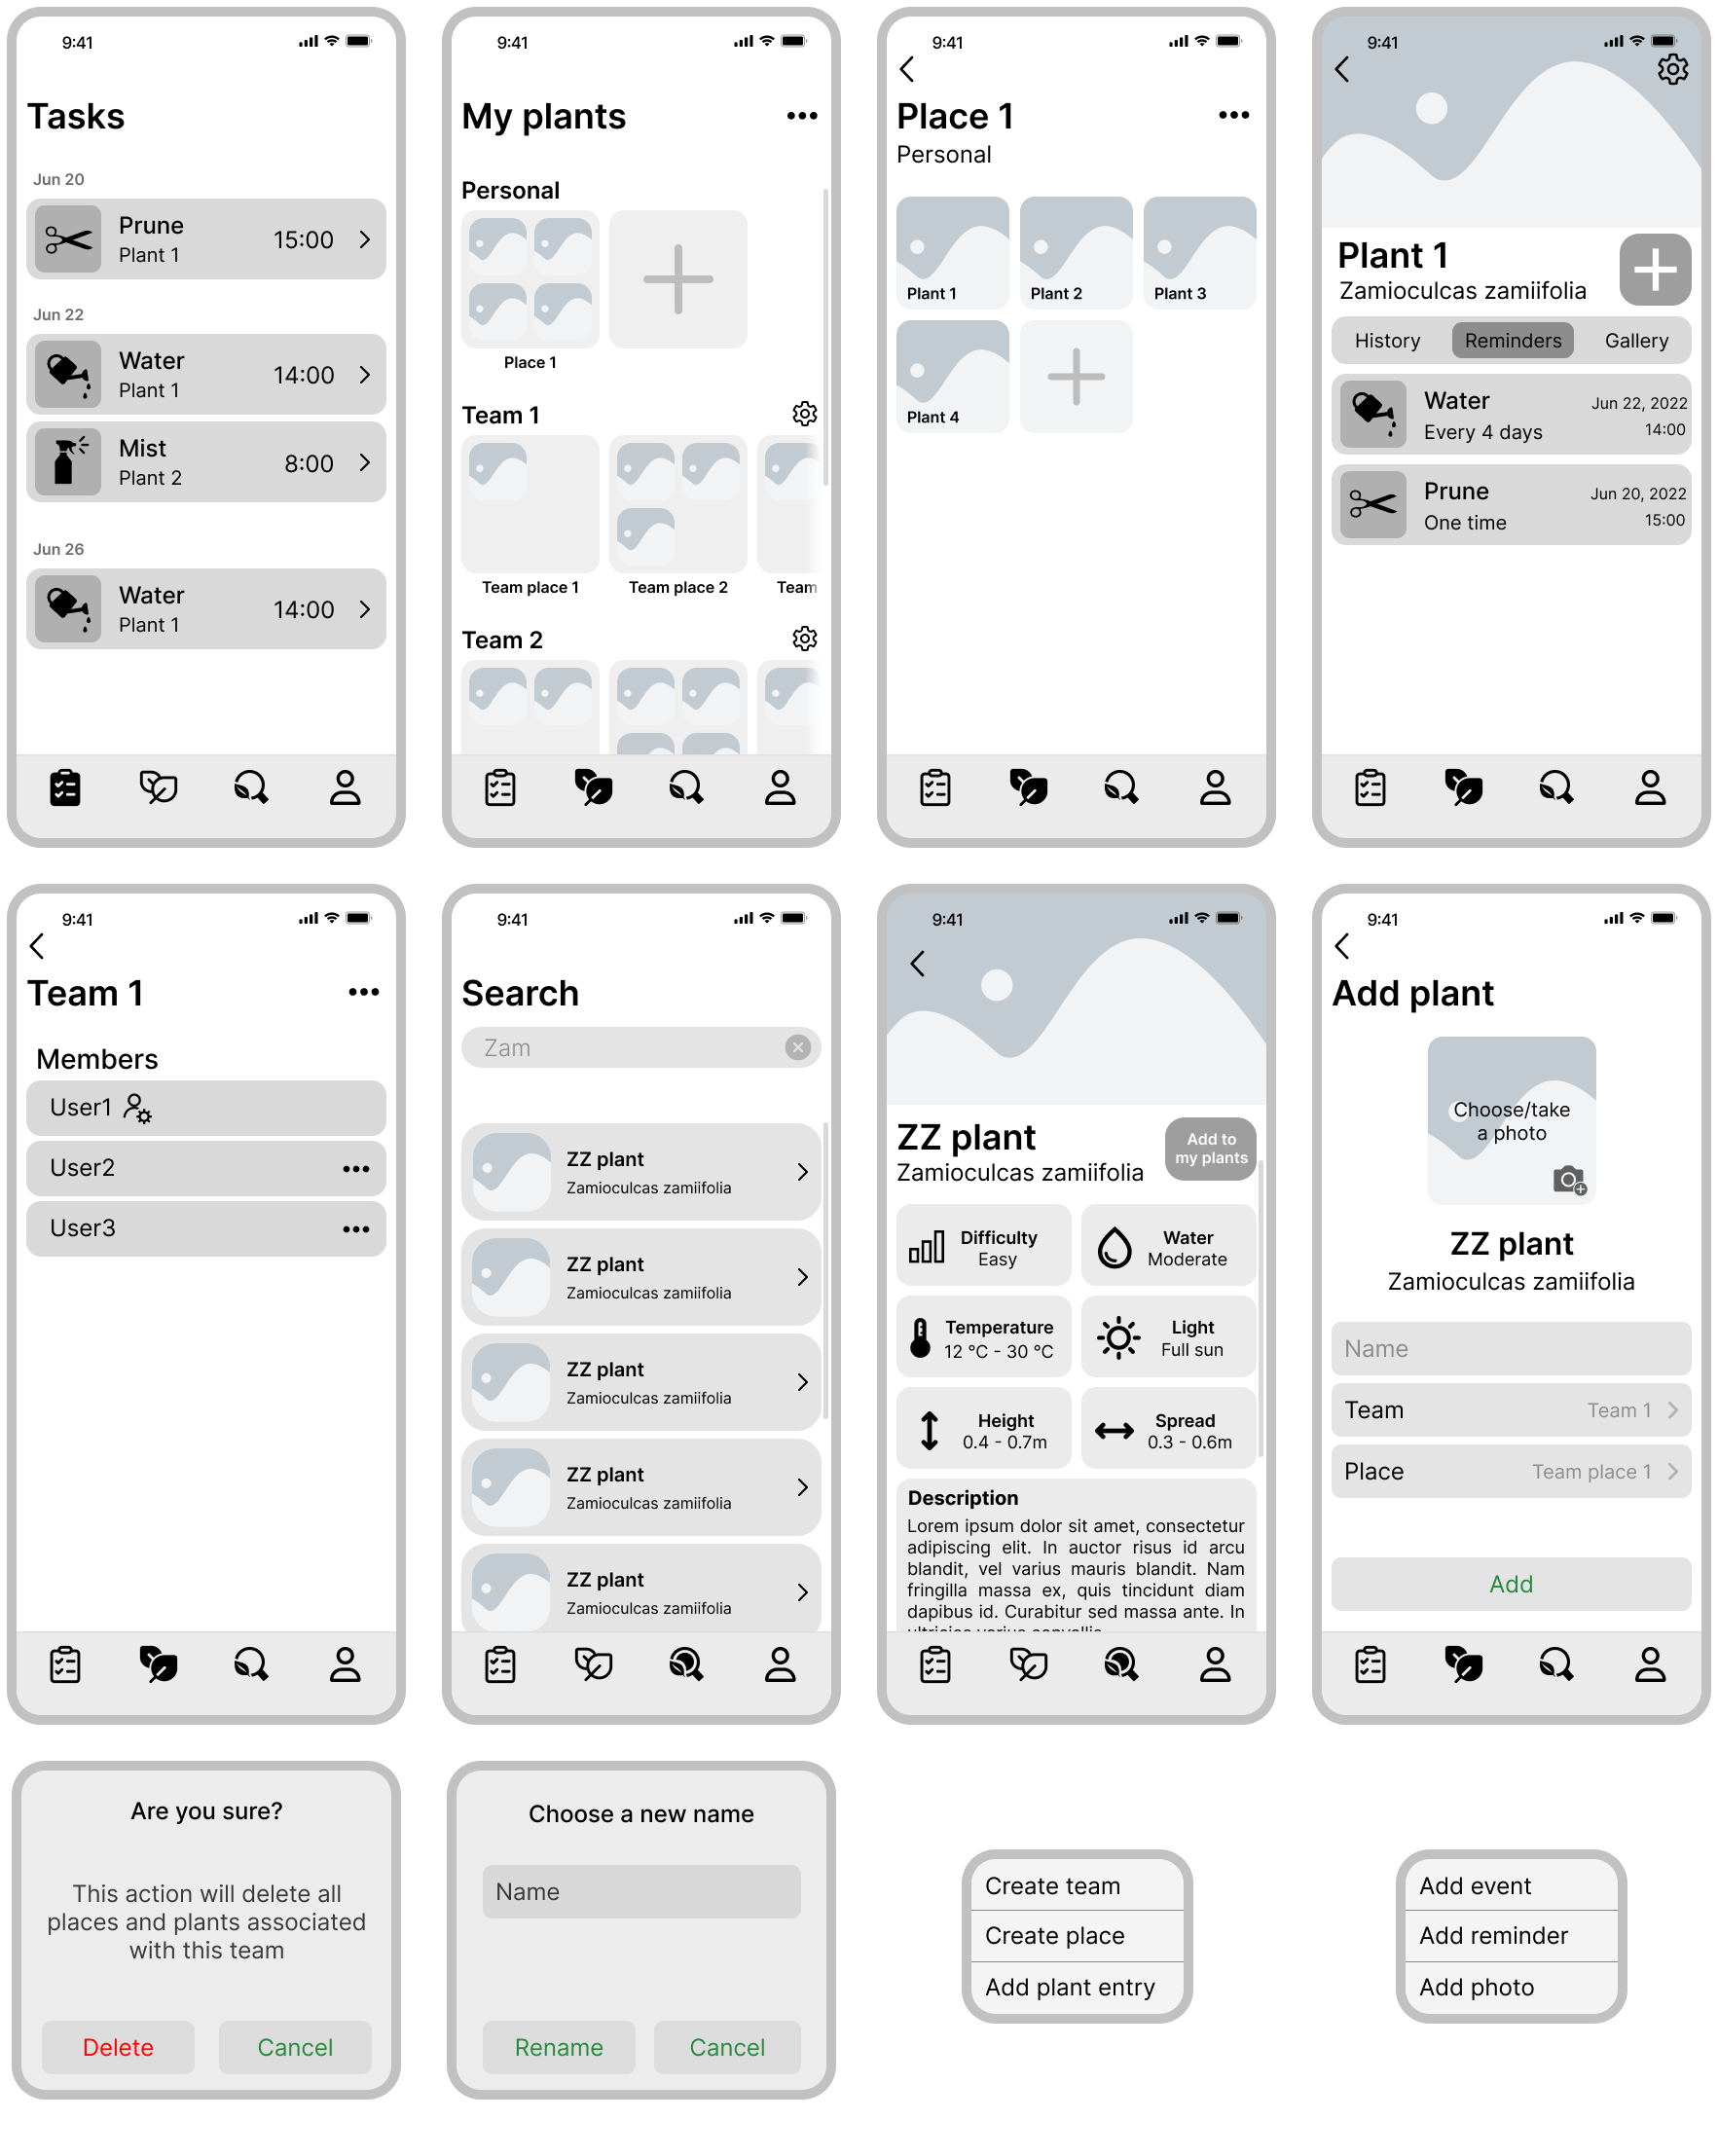
\includegraphics[width=1\linewidth]{images/wireframes.png}
  	\caption{Ukázka obrazovek a kontextových nabídek vytvořeného prototypu}
  	\label{img:prototype-showcase}
\end{figure}

% --------------------------------------------------------------------------------------------

\chapter{Realizace}
\label{ch4}
V~této kapitole je popsána realizace aplikace (vycházející z~návrhu). Je rozdělena do dvou sekci, první se věnuje serverové části a druhá části klientské, tedy mobilní aplikaci pro iOS. Nejprve byla implementována serverová část aplikace se základními koncovými body pro komunikaci (REST API). Ty umožňovali autentizaci a CRUD operace nad jednotlivými entitami, respektive jejich vytvoření, čtení, úprava a mazání. Následně byla podle navrženého uživatelského rozhraní vytvořena mobilní aplikace, přičemž byly v~případě potřeby vytvářeny nové koncové body či dělány další menší úpravy v~serverové části.

Vývoj probíhal s~využitím řady nástrojů, jejichž popis se nachází níže.

\begin{description}
    \item[Visual Studio Code] Jedná se o~bezplatný open source editor zdrojových kódů postavený na frameworku Electrum (multiplatformní desktopové aplikace), který vyvíjen společností Microsoft. V~základu se jedná o~jednoduchý editor, který ale podporuje debuggování, zvýrazňování syntaxe, automatické doplňování či refaktoring. Síla tohoto editoru však tkví v~podpoře doplňků (extensions), které lze pár kliky instalovat a vytvořit tak téměř plnohodnotné vývojové prostředí (IDE). Dle výsledků ankety Developer Survey pro rok 2022  \cite{stackoverflow-survey}, kterou každoročně zpracovává webová stránka Stack Overflow, jde o~nejpoužívanější IDE mezi vývojáři s~podílem $74,48 \%$ \cite{vscode-1, vscode-2}
    \item[Xcode] Pro vývoj nativních aplikací pro zařízení společnosti Apple zde existuje pouze jediné vývojové prostředí a tím je Xcode. Toto vývojové prostředí bylo vytvořeno a je spravováno společností Apple a je ho možné nainstalovat a spustit pouze na zařízeních s~operačním systémem macOS. Nabízí všechny potřebné nástroje a prostředky pro vývoj software na většinu zařízení od společnosti Apple (vývoj pro iOS, iPadOS, macOS, watchOS, tvOS). \cite{xcode}
    \item[Docker] Docker je open-source nástroj pro kontejnerizaci (virtualizace na úrovni operačního systému), doručení a spouštění aplikací na různých platformách. Docker byl v~rámci této závěrečné práce použit pro vytvoření a spuštění kontejneru s~PostgreSQL databází pro vývoj a pro end-to-end testování. \cite{docker-1, docker-2}
    \item[Insomnia] Jde o~open source API klienta, který umožňuje vytvářet, posílat a testovat REST, SOAP, GraphQL a gRPC dotazy. Další součástí je i editor pro tvorbu API dokumentace ve formátu OpenAPI. Tento nástroj byl využit k~ručnímu testování REST dotazů v~průběhu vývoje. \cite{insomnia}
    \item[DataGrip] Nástroj DataGrip od společnosti JetBrains, je integrované vývojové prostředí pro databáze a SQL, s~jehož pomocí se lze připojit k~databázi, psát dotazy, prohlížet data, importovat nebo exportovat data a provádět všechny potřebné manipulace. Vedle nástroje Prisma Studio (prohlížeč databáze, který je součástí Prisma ORM) byl DataGrip použit pro prohlížení a úpravu dat v~databázi během vývoje. \cite{datagrip}
    \item[Git] Git je distribuovaný open source systém pro správu verzí, který umožňuje ukládat kód, sledovat historii revizí, slučovat změny kódu a v~případě potřeby se vracet k~dřívějším verzím kódu. Kód byl za pomoci tohoto systému verzován a samotný repozitář byl uložen na serveru Github. \cite{git}
\end{description}

\section{Serverová část}
Jak již bylo zmíněno v~návrhu, serverová část byla naimplementována ve frameworku NestJs, přičemž pro mapování persistentních dat a práci s~nimi byla využita open source knihovna Prisma. Výsledná souborová struktura této části aplikace je popsána v~\ref{tree:server-file-structure}. Níže v~této sekci se nachází popis dalších využitých knihoven, datového schématu, jednotlivých modulů, klíčových mechanismů a detaily ohledně finálního nasazení.

\begin{figure}
    \centering
    \dirtree{%
        .1 server\DTcomment{adresář se soubory serverové části}.
        .2 prisma\DTcomment{adresář se soubory vztahující se ke knihovně prisma}.
        .3 migrations\DTcomment{adresář s~migračními skripty}.
        .3 schema.prisma\DTcomment{soubor s~definicí databázového schématu}.
        .3 seed.ts\DTcomment{skript pro naplnění databáze}.
        .2 src.\DTcomment{adresář se zdrojovými kódy samotného NestJs projektu}.
        .3 decorators\DTcomment{adresář s~vlastními dekorátory}.
        .3 middleware\DTcomment{adresář s~vlastním middleware}.
        .3 modules\DTcomment{adresář s~moduly}.
        .3 main.ts\DTcomment{hlavní spouštěcí soubor}.
        .2 test\DTcomment{adresář se sadou e2e testů}.
        .2 .env\DTcomment{proměnné prostředí}.
        .2 .eslint.js\DTcomment{ESLint konfigurační soubor}.
        .2 .gitignore\DTcomment{soubory ignorované verzovacím systémem git}.
        .2 .prettierrc\DTcomment{Prettier konfigurační soubor}.
        .2 docker-compose.yml\DTcomment{soubor s~definicemi docker kontejnerů}.
        .2 nest-cli.json\DTcomment{NestJs konfigurační soubor}.
        .2 package-lock.json\DTcomment{soubor s~přesnými informacemi o~závislostech}.
        .2 package.json\DTcomment{manifest závislostí projektu}.
        .2 Procfile\DTcomment{instrukce pro spuštění na platformě Heroku}.
        .2 README.md\DTcomment{základní informace}.
        .2 tsconfig.build.ts\DTcomment{konfigurační soubor pro TypeScript (sestavení)}.
        .2 tsconfig.ts\DTcomment{konfigurační soubor pro TypeScript}.
    }
    \caption{Souborová struktura serverové části}
  	\label{tree:server-file-structure}
\end{figure}

\subsection{Podpůrné knihovny}
Vedle knihoven, se kterými v~základu přichází framework NestJs, bylo využito i několik dalších knihoven, které usnadňují a řeší určité aspekty aplikace. Jedná se zejména o~knihovny usnadňující zabezpečení, validaci dat a odesílání notifikací. Zde se nachází jejich seznam a krátký popis.

\begin{description}
    \item[argon2] Balíček, pomocí kterého lze hashovat data hashovací funkce Argon2, která shrnuje nejnovější poznatky v~oblasti návrhu paměťově náročných funkcí. Tato hashovací funkce byla prohlášena za vítěze soutěže Password Hashing Competition \cite{password-hashing-competition} v~červnu roku 2015 a jejími tvůrci jsou výzkumníci z~Lucemburské univerzity. \cite{argon2}
    \newpage
    \item[node-apn]  Jedná se o~balíček, který podporuje komunikaci a posílání notifikací skrze APNs (Apple Push Notification service). Byl použit komunitně spravovaný fork originálního balíčku, neboť ten již není aktivně vyvíjen. \cite{node-apn}
    \item[class-transformer, class-validator] Balíčky pro transformaci plain objektů na instance tříd a validaci proměnných tříd pomocí dekorátorů. Tyto balíčky následně využívá NestJs ve svých \textit{Validation Pipes}, které zajišťují automatickou validaci jednotlivých dotazů. \cite{class-transformer, class-validator}
    \item[helmet] Helmet je kolekcí menších middlewarových funkcí pro aplikace založené na Express.js (s~nímž NestJs v~základu pracuje), které nastavují HTTP hlavičky. Tím lze ochránit aplikace před některými známými webovými zranitelnostmi. \cite{helmet}
    \item[parse-duration] Balíček pro konverzi řetězců popisující dobu trvání (v~lidsky čitelné podobě) na milisekundy. Příkladem buď například výraz \uv{1h} nebo \uv{30m 10s}. \cite{parse-duration}
    \item[passport] Autentizační middleware pro Node.js, kompatibilní s~Express.js. Jeho účelem je ověřování požadavků, které provádí prostřednictvím pluginů, které jsou známy pod pojmem strategie. Mezi ně patří například přihlašování uživatelským jménem a heslem, pomocí OAuth nebo OpenID či autentizaci skrz tokeny.
    \item[pactum] Balíček pro automatizaci testování REST API vhodný pro nejrůznější druhy testů, včetně integračních či end to end. \cite{pactum}
    \label{pactum}
\end{description}

\subsection{Databázové schéma}
V~souboru \textit{schema.prisma} byly popsány jednotlivé modely (entity) a vztahy mezi nimi. Následně byl z~tohoto schématu pomocí Prisma vygenerován migrační skript, který dokáže zanést dané schéma do zvolené databáze (vytvoří příslušné tabulky). Pokud by bylo potřeba udělat ve schématu nějaké změny, je možné vygenerovat další migrační skript, který dokáže aplikovat pouze změny nového schématu oproti starému. Daná migrace pak byla aplikována na instanci PostgreSQL databáze, která běžela v~Docker kontejneru na mém počítači. Současně s~aplikováním migrace byl vygenerován klient, který na základě daného schématu obsahuje rozhraní (včetně typů), pomocí kterého se lze připojit k~databázi a provádět databázové operace s~definovanými modely (entitami). Výsledná struktura databáze PostgreSQL po aplikování migrace je zobrazena na obrázku \ref{img:db-structure}.

\begin{figure}
	\centering
	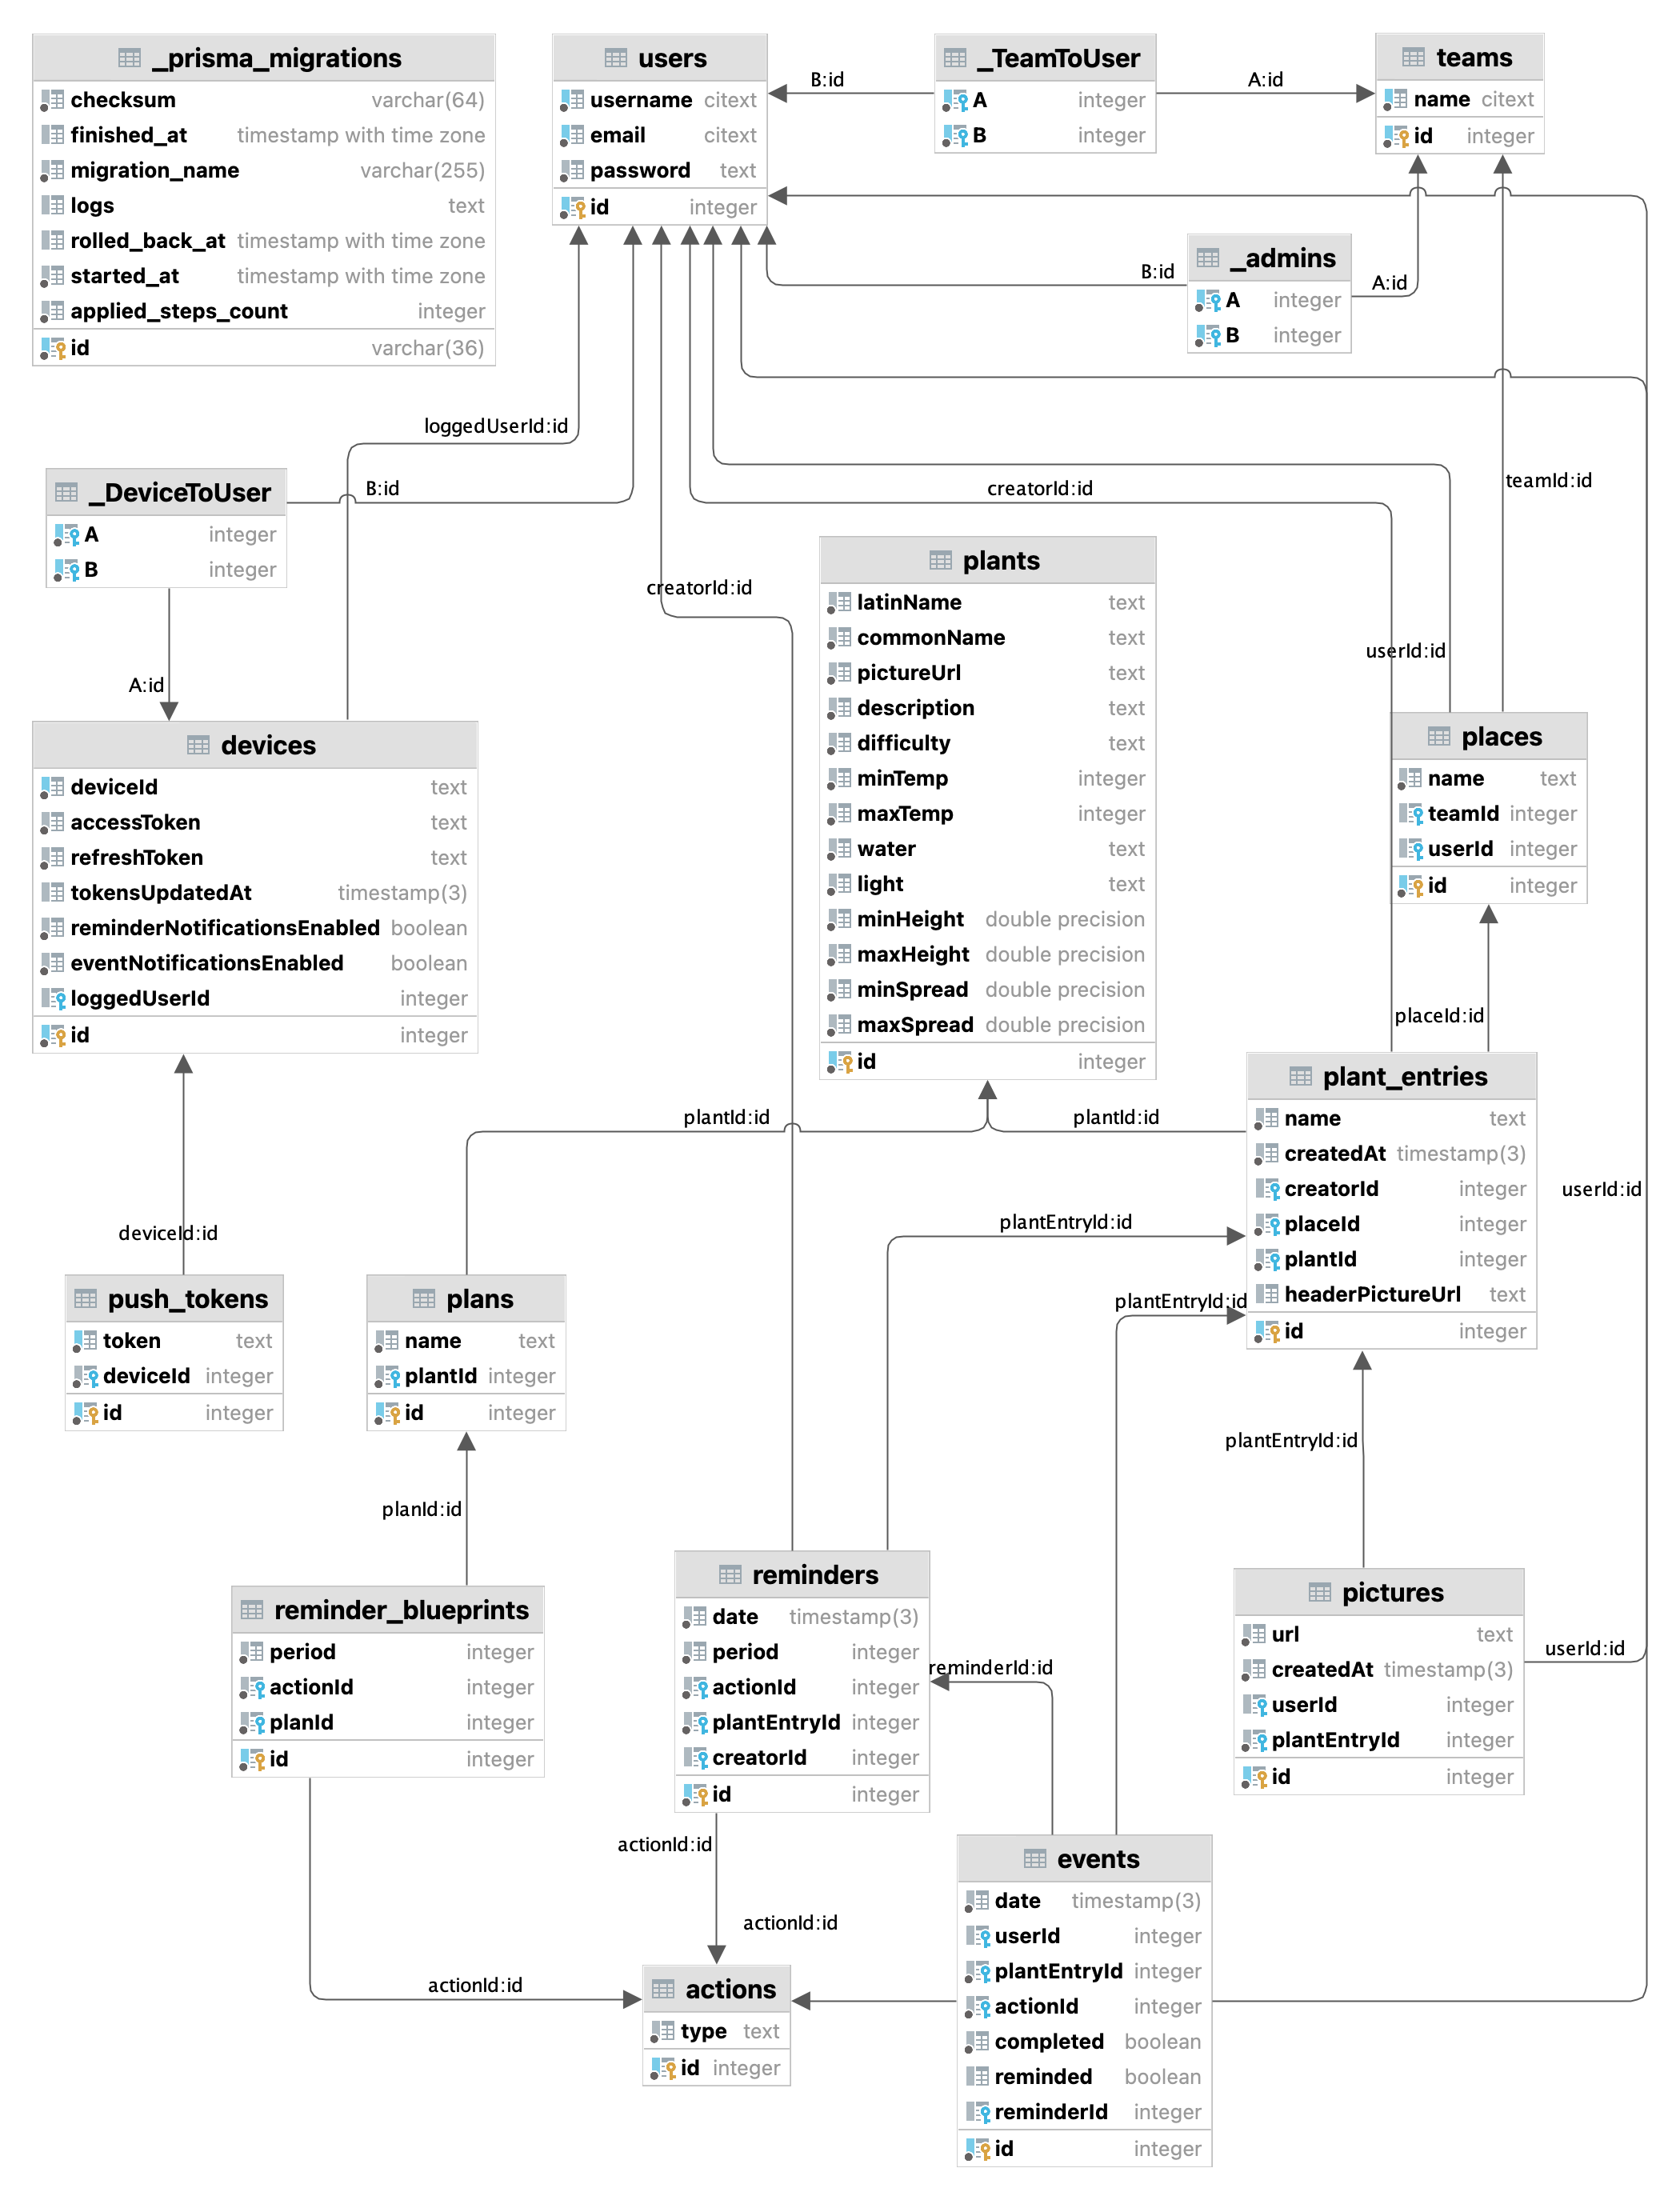
\includegraphics[width=1\linewidth]{images/db-structure.png}
  	\caption{Struktura databáze}
  	\label{img:db-structure}
\end{figure}

\subsection{Moduly}
Aplikace používá celkem 14 modulů. Hlavním modulem je \textit{App}, který obsahuje veškeré zbylé moduly. Jeho součástí je zaregistrování již připraveného modulu \textit{Schedule}, který zprostředkovává funkcionality kolem pravidelného volání funkcí. Ten je poté využit k~posílání připomínkových notifikací. Vedle hlavního \textit{App} modulu běží modul \textit{Swagger}, který automaticky generuje \mbox{OpenAPI} dokumentaci z~kódu. Ta se nachází na cestě \texttt{/docs}. Níže jsou popsány moduly, které jsou součástí hlavního modulu \textit{App}.

\subsubsection{Prisma}
Klíčový modul, který zprostředkovává ostatním modulům \textit{PrismaService}, což je provider umožňující použití vygenerovaného Prisma klienta. Jeho definici lze vidět v~kódu \ref{code:prismaservice}. PrismaService dědí od třídy PrismaClient (vygenerovaný klient) a implementuje OnModuleInit (v~metodě onModuleInit, která je volána při inicializaci modulu, dojde k~připojení klienta do databáze).

\begin{listing}
    \inputminted{javascript}{code/prismaservice.txt}
    \caption{Třída PrismaService}
    \label{code:prismaservice}
\end{listing}

\subsubsection{Auth}
Modul zodpovědný za autentizaci uživatelů. Podle návrhu byla implementována autentizace pomocí JWT, kdy po úspěšné registraci či přihlášení je vygenerována dvojice tokenů, které opravňují uživatele dotazovat se na zbylých koncových bodech. Tyto tokeny jsou uloženy do databáze k~příslušnému zařízení (device). Byly vytvořeny 2 autentizační strategie \textit{JwtAccessTokenStrategy} a \textit{JwtRefreshTokenStrategy}, které dědí od již připravené třídy PassportStrategy a implementují metodu \textit{validate}. Ta definuje, zda má dotaz v~\textit{Authorization} hlavičce validní access, respektive refresh token. Tyto strategie jsou následně použity v~třídách \textit{JwtAccessTokenGuard} a \textit{JwtRefreshTokenGuard}, které umožňují controllerům pomocí dekorátoru specifikovat, že se má použít daná autentizace. Zpřístupněny jsou tyto koncové body:

\begin{description}
    \item[POST /auth/register] Registrace nového uživatele. 
    \item[POST /auth/login] Přihlášení uživatele.
    \item[POST /auth/refresh] Obnova tokenu.
    \item[POST /auth/logout] Odhlášení uživatele (zneplatnění tokenů).
\end{description}

\subsubsection{User}
Poskytuje rozhraní pro správu uživatelů. Provider \textit{UserService} je využit v~modulu Auth pro vytváření uživatelů. Controller v~tomto modulu spravuje tyto koncové body:

\begin{description}
    \item[GET /users] Získání všech uživatelů.
    \item[GET /users/\{id\}] Získání konkrétního uživatele.
    \item[DELETE /users/delete] Smazání uživatele (id uživatele, který bude smazán, se nachází v~access tokenu).
\end{description}

\subsubsection{Team}
Zprostředkovává správu týmů, včetně vytváření, získávání, editace, mazání, přidávání a odebírání členů, udělování a odebírání práv. Dostupné endpointy jsou:

\begin{description}
    \item[POST /teams] Vytvoření nového týmu.
    \item[GET /teams] Získání všech týmů, jichž je přihlášený uživatel členem.
    \item[GET /teams/summary] Získání souhrnu všech týmů, jichž je přihlášený uživatel členem. Tento souhrn obsahuje přímo i informace o~místech a záznamech rostlin. Tento endpoint slouží pro získání všech potřebných informací v~mobilní aplikace na obrazovce \uv{My Plants}.
    \item[GET /teams/\{id\}] Získání konkrétního týmu.
    \item[PUT /teams/\{id\}] Editace konkrétního týmu.
    \item[DELETE /teams/\{id\}] Smazání konkrétního týmu.
    \item[GET /teams/\{id\}/members] Získání všech členů (uživatelů) konkrétního týmu.
    \item[POST /teams/\{id\}/members] Přidání uživatele mezi členy týmu.
    \item[DELETE /teams/\{id\}/members/\{id\}] Odebrání uživatele z~týmu.
    \item[POST /teams/\{id\}/members/give-admin-rights] Přidání uživatele mezi členy týmu.
    \item[POST /teams/\{id\}/members/remove-admin-rights] Přidání uživatele mezi členy týmu.
\end{description}

\subsubsection{Place}
Modul pro spravování míst. Protože místo může patřit buď samotnému uživateli nebo týmu, bylo potřeba vytvořit dva separátní koncové body pro vytváření. Pomocí jednoho lze vytvořit místo patřící ke konkrétnímu uživateli (osobní) a pomocí druhého místo, které patří týmu. Koncovými body jsou:

\begin{description}
    \item[POST /places/user] Vytvoření nového místa pro uživatele.
    \item[POST /places/team] Vytvoření nového místa pro tým.
    \item[GET /places] Získání všech míst.
    \item[GET /places/\{id\}] Získání konkrétního místa.
    \item[PUT /places/\{id\}] Editace konkrétního místa.
    \item[DELETE /places/\{id\}] Smazání konkrétního místa.
\end{description}

\subsubsection{Plant}
Jednoduchý modul pro získávání různých druhů rostlin. V~odpovědích jsou posílány i jednotlivé připomínkové plány. Endpointy jsou následující:

\begin{description}
    \item[GET /plants] Získání všech rostlin.
    \item[GET /plants/\{id\}] Získání konkrétní rostliny.
\end{description}

\subsubsection{PlantEntry}
Modul pro správu záznamů rostlin. Základní operace s~danou entitou plus endpoint na nastavení připomínkového plánu. Koncové body:

\begin{description}
    \item[POST /plant-entries] Vytvoření záznamu rostliny.
    \item[GET /plant-entries] Získání všech záznamů rostlin.
    \item[GET /plant-entries/\{id\}] Získání konkrétního záznamu rostliny.
    \item[PUT /plant-entries/\{id\}] Editace konkrétního záznamu rostliny.
    \item[DELETE /plant-entries/\{id\}] Smazání konkrétního záznamu rostliny.
    \item[POST /plant-entries/\{id\}/setPlan] Nastavení připomínkového plánu konkrétnímu záznamu rostliny.
\end{description}

\subsubsection{Event}
Tento modul řeší vytváření, získávání, úpravu a mazání událostí. Má přístup k~modulům Prisma, User (vyhledání uživatelů, pro které je daná událost relevantní) a Notification (posílání notifikací). Zpřístupněnými koncovými body jsou:

\begin{description}
    \item[POST /events] Vytvoření nové události, která je označená jako provedená.  Při vytvoření nové události je poslána notifikace ostatním členům v~týmu, kteří mají povolené \textit{event} notifikace.
    \item[GET /events] Získání událostí. Query parametrem lze vyfiltrovat pouze dokončené nebo nedokončené události.
    \item[GET /events/\{id\}] Získání konkrétní události.
    \item[PUT /events/\{id\}] Editace konkrétní události.
    \item[DELETE /events/\{id\}] Smazání konkrétní události.
\end{description}

\subsubsection{Reminder}
Tento modul slouží pro vytváření, získávání, úpravu a mazání připomínek. Zpřístupněné endpointy jsou:

\begin{description}
    \item[POST /reminders] Vytvoření připomínky.
    \item[GET /reminders] Získání všech připomínek, které patří přihlášenému uživateli.
    \item[GET /reminders/\{id\}] Získání konkrétní připomínky.
    \item[PUT /reminders/\{id\}] Editace konkrétní připomínky.
    \item[DELETE /reminders/\{id\}] Smazání konkrétní připomínky.
\end{description}

\subsubsection{Picture}
Vytváření, získání, úprava a mazání obrázků. Jednotlivé obrázky se nahrávají na cloudové úložiště Firebase Storage přímo v~klientské části aplikace a zde se vytváří pouze záznam s~odkazem na zdroj, kde je obrázek uložen. Jednotlivé koncové body jsou následující:

\begin{description}
    \item[POST /pictures] Vytvoření nového obrázku záznamu rostliny.
    \item[GET /pictures] Získání všech obrázků.
    \item[GET /pictures/\{id\}] Získání konkrétního obrázku.
    \item[DELETE /pictures/\{id\}] Smazání konkrétního obrázku.
\end{description}

\subsubsection{Notification}
Modul, který zprostředkovává nastavení a posílání notifikací uživatelům. Provider \textit{NotificationService} poskytuje funkci \textit{sendEventNotification}, která umožňuje poslat event notifikaci. Tuto funkci poté využívá provider \textit{EventService} v~\textit{Event} modulu. Také je zde definována pravidelná úloha (Cron) \textit{handleReminderNotifications}, která se stará o~posílání připomínkových push notifikací. Kontrola připomínek probíhá každou minutu. Notifikace je poslána pomocí balíčku \textit{node-apn} Kód této úlohy je vidět na \ref{code:notification-cron}. Zároveň jsou poskytnuty následující endpointy:

\begin{description}
    \item[POST /notifications/addPushToken] Přidání \uv{push} tokenu, který je unikátní pro každé iOS zařízení a je zřízeno po zaregistrování daného zařízení k~push notifikacím.
    \item[POST /notifications/enable-reminder-notifications] Zapnutí připomínkových notifikací.
    \item[POST /notifications/disable-reminder-notifications] Vypnutí připomínkových notifikací.
    \item[POST /notifications/enable-event-notifications] Zapnutí notifikací o~provedení události.
    \item[POST /notifications/disable-event-notifications] Vypnutí notifikací o~provedení události.
\end{description}

\begin{listing}
    \inputminted{javascript}{code/notifications-cron.txt}
    \caption{Pravidelná úloha, která posílá připomínkové notifikace}
    \label{code:notification-cron}
\end{listing}

\subsection{End to end testy}
Pro kontrolu fungující aplikace, byla vytvořena základní sada end to end testů (E2E), která testuje autentizaci a CRUD operace nad entitou user. End to end testy kontrolují, jestli aplikace funguje jako celek tak, za jakým účelem byla vytvořena (testuje komplexní procesy z~pohledu uživatele). V~kontextu implementované aplikace (serverová část) se tedy jedná o~správné odbavování požadavků a vracení správných odpovědí pro dané vstupy.

Pro toto testování je tedy nutné spustit aplikaci včetně databáze, do které má během testů přístup. Testy používají balíček \textit{Jest} \cite{jest}, který je výchozím testovacím frameworkem NestJs projektu, a dále také balíček \textit{PactumJS} (viz \ref{pactum}) pro jednoduché a efektivní testování samotného rozhraní REST. Testovací databáze ve formě Docker kontejneru je vytvořena před samotným během testů a ta je navíc naplněna testovacími daty. Příkladem testu, který testuje správnou registraci uživatele, buď kód \ref{code:test-example}.

\begin{listing}
    \inputminted{javascript}{code/test-example.txt}
    \caption{Příklad testu ověřující validní registraci uživatele}
    \label{code:test-example}
\end{listing}

\subsection{Nasazení}
Pro nasazení aplikace do ostrého provozu byla použita platforma jako služba (PaaS) Heroku \cite{heroku}. Aplikace jsou nasazovány na virtuální počítače (na stroje poskytované Amazon Web Services), v~Heroku terminologii zvané jako \textit{dynos}. Tyto virtuální počítače mají přiděleny prostředky (výkon) podle plánu, který si uživatel zvolí (a zaplatí). Protože se jedná o~PaaS, není potřeba se starat o~infrastrukturu strojů, na samotných \textit{dynos} je už připravené prostředí pro spuštění aplikací nejrůznějších technologií. Stačí doručit kód (například skrze GitHub) a specifikovat instrukce (Procfile), které aplikaci spustí. Dalším důvodem, mimo jednoduchost nasazení, je také fakt, že Heroku nabízí i hosting PostgreSQL databáze. Heroku tedy stačí na kompletní nasazení aplikace a databáze.

Do 28. listopadu 2022 nabízela služba Heroku omezené bezplatné plány, které stačily na základní experimenty či malé projekty. Z~finančních důvodů však tyto plány byly odstraněny a nahrazeny novými placenými (avšak cenově dostupnými) plány. Heroku zároveň ale podporuje studenty a nabízí jim kredity v~ceně 156 dolarů (ekvivalent 13 kreditů za každý měsíc po dobu jednoho roku), které lze jakkoliv využít na různé plány. Aby daný student kredity dostal, je potřeba se ověřit GitHub účtem, který má přístup k~\textit{Github Student Developer} balíku. Tento balík lze získat propojením GitHub účtu s~univerzitním účtem. Tato nabídka byla využita a bylo zřízeno \textit{dyno} (v~plánu basic) na provoz serverové části aplikace a PostgreSQL databáze (v~plánu mini). V~kontextu serverové části byly nastaveny veškeré proměnné prostředí k~úspěšnému připojení k~produkční PostgreSQL databázi (url databáze), posílání notifikací skrze APNs (bundle id, key, team id, druh prostředí) a také byly nastaveny expirační doby access (1 hodina) a refresh (7 dní) tokenu. Databáze byla také zároveň naplněna celkem šestnácti druhy rostlin.

V~GitHub repozitáři byl v~rámci GitHub Actions zřízena akce pro spuštění jednotkových (unit) a E2E testů a následného nasazení aplikace na Heroku (na již vytvořené a připravené \textit{dyno}). Tato akce se spouští vždy při odeslání (push) kódu na hlavní větev repozitáře nebo manuálně kliknutím na webu. Akce (jobs) jsou definovány v~souboru \textit{backend-test-and-deploy.yml}, který je umístěn v~adresáři \textit{.github/workflows}. Tento adresář se musí nacházet v~kořeni repozitáře, aby GitHub konfigurace akcí rozeznal.

\section{Klientská část}
Aplikace byla implementována dle návrhu ve frameworku SwiftUI s~použitím několika dalších knihoven. Vzhled aplikace vychází ze zhotoveného Hi-Fi prototypu, ve kterém byly provedeny místy menší úpravy a vylepšení. Souborová struktura aplikace se nachází na \ref{tree:client-file-structure}.

\begin{figure}[H]
    \centering
    \dirtree{%
        .1 client-ios\DTcomment{adresář se soubory klientské části}.
        .2 sprinkled-ios\DTcomment{samotná mobilní aplikace}.
        .3 Assets\DTcomment{adresář s~prostředky (obrázky, barvy, ikony)}.
        .3 Services\DTcomment{adresář se službami vkládané pomocí DI}.
        .3 States\DTcomment{adresář se stavy předávané jako objekty prostředí}.
        .3 Model\DTcomment{adresář s~Modely}.
        .3 ViewModel\DTcomment{adresář s~ViewModely}.
        .3 View\DTcomment{adresář s~obrazovkami (Views)}.
        .3 AppDelegate.swift \DTcomment{třída pro zpracovávání událostí životního cyklu aplikace}.
        .3 Errors.swift\DTcomment{chyb (výjimky)}.
        .3 Extensions.swift\DTcomment{rozšíření}.
        .3 ImagePicker.swift\DTcomment{obrazovka pro výběr obrázků}.
        .3 LaunchScreen.storyboard\DTcomment{načítací obrazovka}.
        .3 sprinkled-ios.entitlements\DTcomment{oprávnění}.
        .3 SprinkledApp.swift\DTcomment{hlavní třída aplikace}.
        .3 Styles.swift\DTcomment{styly}.
        .3 TestData.swift\DTcomment{testovací data}.
        .3 UIElements.swift\DTcomment{grafické prvky}.
        .3 Utils.swift\DTcomment{pomocné funkce}.
        .2 sprinkled-ios-tests\DTcomment{jednotkové testy}.
        .2 sprinkled-ios.xcodeproj\DTcomment{soubor s~konfigurací projektu}.
    }
    \caption{Souborová struktura klientské části}
  	\label{tree:client-file-structure}
\end{figure}

\subsection{Podpůrné knihovny}
Aplikace používá několik knihoven, které usnadňují práci, umožňují používat externí služby či přidávají grafické prvky nebo funkcionality. Těmito knihovnami jsou:

\begin{description}
    \item[Kingfisher] Knihovna pro práci se vzdálenými obrázky. Umožňuje stahování, zobrazování a ukládání obrázků z~webu do mezipaměti. Výhodou je, že již stažené obrázky se nemusí opakovaně stahovat, pokud se v~mezipaměti nachází. Samotná konfigurace ukládání a limity lze přizpůsobit, ale v~mnoha případech stačí použít výchozí nastavení. \cite{kingfisher}
    \item[Firebase iOS SDK] Sada komponent pro práci s~\textit{Firebase}. V~rámci \textit{Firebase} byl využit nástroj \textit{Firebase Storage} pro ukládání obrázků/fotografií.
    \item[Swift Collections] Balíček (o~který se stará samotný Apple), který obsahuje několik doplňujících datových struktur, které nejsou součástí \textit{Swift Standard Library}. Jedná se o~obousměrnou frontu, seřazenou množinu a slovník (v~nadcházejících verzích i například bitová množina a pole či prioritní fronta). Právě seřazený slovník je využit na obrazovce \textit{Tasks}, ve kterém jsou uchovány nadcházející úkoly. \cite{swift-collections}
    \item[JWTDecode] Knihovna pro dekódování JWT tokenu. Z~textového řetězce je vytvořen objekt, ze kterého lze jednoduše získávat informace obsažené v~tokenu. \cite{jwtdecode}
    \item[PopupView] Knihovna, která poskytuje několik druhů vyskakovacích a plovoucích oken, které lze různě konfigurovat. S~pomocí této knihovny byly vytvořeny chybové a potvrzovací hlášky. \cite{popupview}
    \item[SwiftUI-Shimmer] Jednoduchý View modifikátor, který danému View přidá \uv{blyštící} se animaci, která se výborně hodí k~reprezentaci načítajících se grafických prvků (spolu s~použitím modifikátoru \textit{redacted}). \cite{swiftui-shimmer}
\end{description}

\subsection{Dependency Injection}
Dependency Injection (Vkládání závislostí) je technika pro předávání závislostí mezi třídami. Tato technika je svázána s~návrhovým vzorem Inversion of Control, ve kterém je cílem uvolnit pevné vazby mezi objekty. V~dependency injection existuje tzv. injektor, což je třída, která je zodpovědná za konstrukci, uchovávání a následnému vkládání instancí tříd (\textit{services}) jiným třídám.

Velice jednoduchá a elegantní implementace tohoto mechanismu byla převzata z~\cite{di}. Struktura \texttt{DependencyInjector} \ref{code:di-injector} obsahuje slovník, do kterého jsou ukládány jednotlivé instance objektů, které je potřeba vkládat jiným objektům. Dále obsahuje metody \texttt{register} pro registraci instancí (vloží ji do slovníku pod klíčem jména třídy) a \texttt{resolve} pro jejich získávání. Vedle této struktury jsou definována dvoje obalení proměnné (property wrappers) \ref{code:di-property-wrappers} -- \texttt{Inject} a \texttt{Provider}, které tyto metody používají, a slouží právě k~samotné registraci a vkládání závislostí.

V~aplikaci je pak vkládání závislostí pomocí této implementace řešeno tak, že po úspěšném spuštění aplikace jsou vytvořeny a zaregistrovány (v~třídě \texttt{AppDelegate}) potřebné služby (services) pomocí obalení proměnné \texttt{Provider}. Následně v~jednotlivých ViewModelech, které danou závislost potřebují, je vytvořena proměnná a přidáno obalení \texttt{Inject}. Tím je do dané proměnné vložen objekt ze seznamu závislostí v~injektoru a lze s~ním jakkoliv nakládat.

\begin{listing}
    \inputminted{swift}{code/di-injector.txt}
    \caption{Třída DependencyInjector, která spravuje závislosti.}
    \label{code:di-injector}
\end{listing}

\begin{listing}
    \inputminted{swift}{code/di-property-wrappers.txt}
    \caption{Vytvoření obalení proměnných (property wrappers) pro jednoduchou registraci služeb (services) a vkládání závislostí.}
    \label{code:di-property-wrappers}
\end{listing}

Služby, které byly vytvořeny a jsou takto dostupné vkládáním, jsou tyto:

\begin{description}
    \item[API] Slouží pro komunikaci se serverovou částí aplikace pomocí REST API. Posílá HTTP požadavky a v~odpovědích získává data ke zobrazení.
    \item[StorageManager] Služba pro ukládání obrázků/fotografií na cloudové uložiště Firebase Storage. Obsahuje jedinou metodu \texttt{uploadImage}, která komprimuje a nahraje obrázek ve formátu JPEG a vrátí URL adresu, na které je daný obrázek dostupný. Kód lze vidět na \ref{code:storage-manager}.
    \item[NotificationManager] Služba, která spravuje notifikace. Pomocí této služby lze požádat o~povolení notifikací a také zapínat a vypínat jednotlivé druhy notifikací (připomínkové a událostní).
\end{description}

\begin{listing}
    \inputminted{swift}{code/storage-manager.txt}
    \caption{Protokol a třída NotificationManager, která umožňuje ukládat obrázky na cloudové uložiště Firebase Storage.}
    \label{code:storage-manager}
\end{listing}

\subsection{Identita a grafické prvky}
Logo aplikace je černé písmeno \uv{S} na bílém pozadí. Na vrchním konci písmena se pak nachází menší zelený list. Vedle tohoto loga bylo vytvořeno logo textové, které neobsahuje pouze první písmeno názvu, ale název celý. To je použito na přihlašovací a registrační obrazovce. Loga lze vidět na obrázku \ref{img:app-logos}.

\begin{figure}[H]
	\centering
	
\includegraphics[width=0.65\linewidth]{images/app-logos.png}
  	\caption{Klasické a textové logo}
  	\label{img:app-logos}
\end{figure}

Aplikace je laděna do kombinace 4 hlavních barev -- černá, bílá, šedá, zelená. Zelená barva je použita zejména pro prvky, se kterými lze nějakým způsobem interagovat (poklepat na ně), nebo pro indikaci aktivních prvků (vybraný tab, sekce). Šedá barva slouží jako pozadí některých prvků a také jako barva informativního textu. Zároveň jsou v této barvě zobrazeny načítající se objekty. Text a pozadí má barvu černou a bílou (záleží na zvoleném barevném režimu -- světlý nebo tmavý). Font textu je ponechán základní, tedy \textit{SF Pro}. Barvu, kterou lze také nalézt, je červená. Ta se nachází na některých tlačítkách, které provádějí destruktivní akce (mazání), a jako pozadí chybových hlášek.

Aplikace používá ve většině případech základní grafické prvky, které jsou přítomny ve \textit{SwiftUI}. Některé tyto prvky ale nevyhovovaly, co se týče grafického provedení (nedají se vhodně stylizovat), a tak byly vytvořeny vlastní verze těchto prvků (tab bar, segmented control). Zároveň byly vytvořeny ty, které se v základu vůbec nenacházejí (vlastní modal). Pro chybové hlášky byl využit balíček \textit{PopupView}. Různé grafické prvky aplikace jsou zobrazeny na obrázku \ref{img:gui-elements}.

\begin{figure}[H]
	\centering
	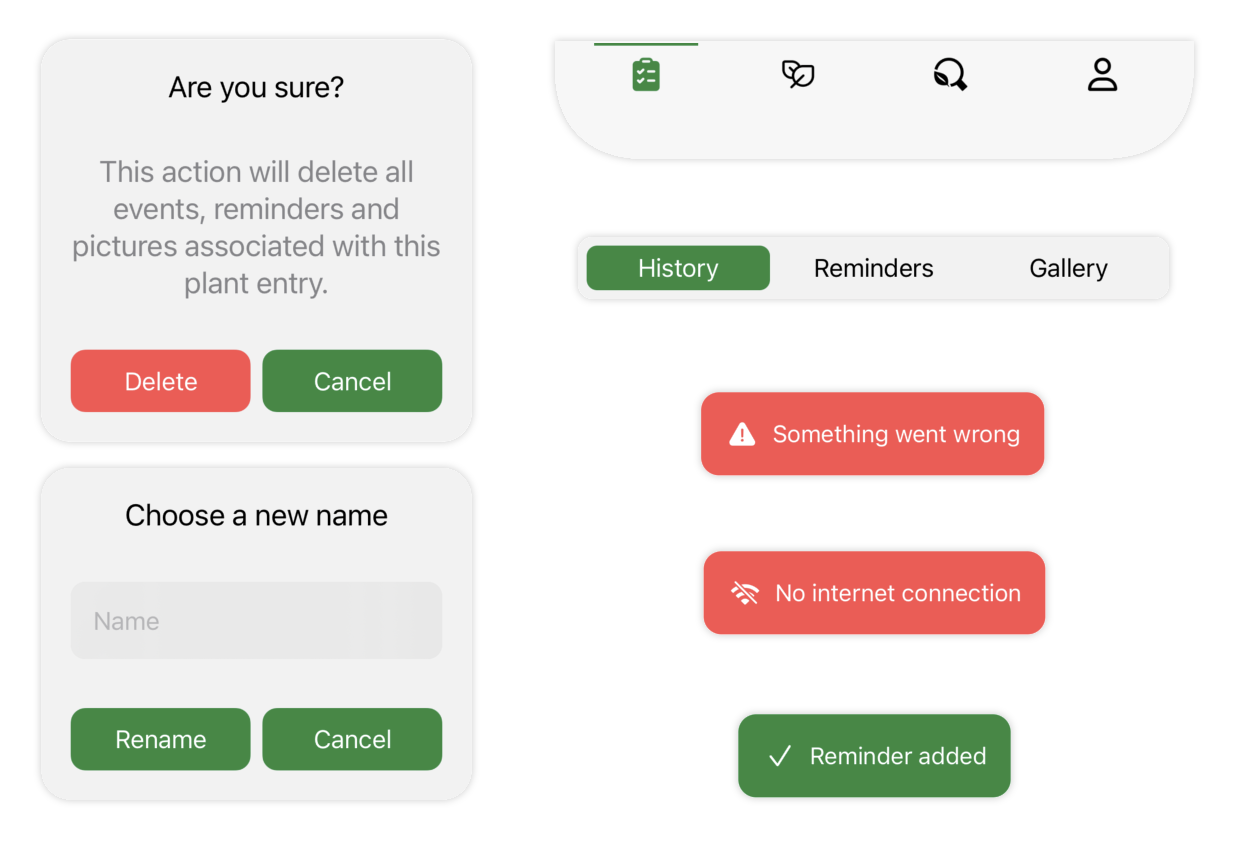
\includegraphics[width=1\linewidth]{images/gui-elements.png}
  	\caption{Ukázka grafických prvků}
  	\label{img:gui-elements}
\end{figure}

\subsection{Přihlášení a registrace}
Přihlašovací a registrační obrazovku lze vidět na ukázce \ref{img:screenshots-2}. Na vrchu obou obrazovek se nachází textové logo a pod ním textová pole pro vyplnění přihlašovacích či registračních informací. Protože rozkliknutí textového pole otevře klávesnici, bylo potřeba zajistit, aby uživatel viděl, co píše a mohl se mezi textovými poli přepínat. U~přihlašovací obrazovky klávesnice nijak neinterferuje s~textovými poli. U~registrace bylo přidáno schovávání loga při otevřené klávesnici. Pokud by logo zůstalo, dolní textová pole by byla překryta klávesnicí.

\subsection{Onboarding}
Cílem onboardingu je seznámit nového uživatele s~funkcemi aplikace a nabídnout mu možnost povolení notifikací. Skládá se celkem ze šesti částí, přičemž tlačítkem \uv{Next} se uživatel může posunout vpřed. Může zároveň také použít \textit{swipe} gesto, kterým se může dostat jak na následující tak na předchozí část. V~poslední části onboardingu se text tlačítka změní na \uv{Get Started}, které onboarding zavře a přesune uživatele do aplikace. Nad tlačítkem se nachází ukazatel, který pomocí teček ukazuje počet částí a v~které části se uživatel právě nachází. Ukázka onboardingu se nachází na obrázku \ref{img:screenshots-1}.

\begin{figure}
	\centering
	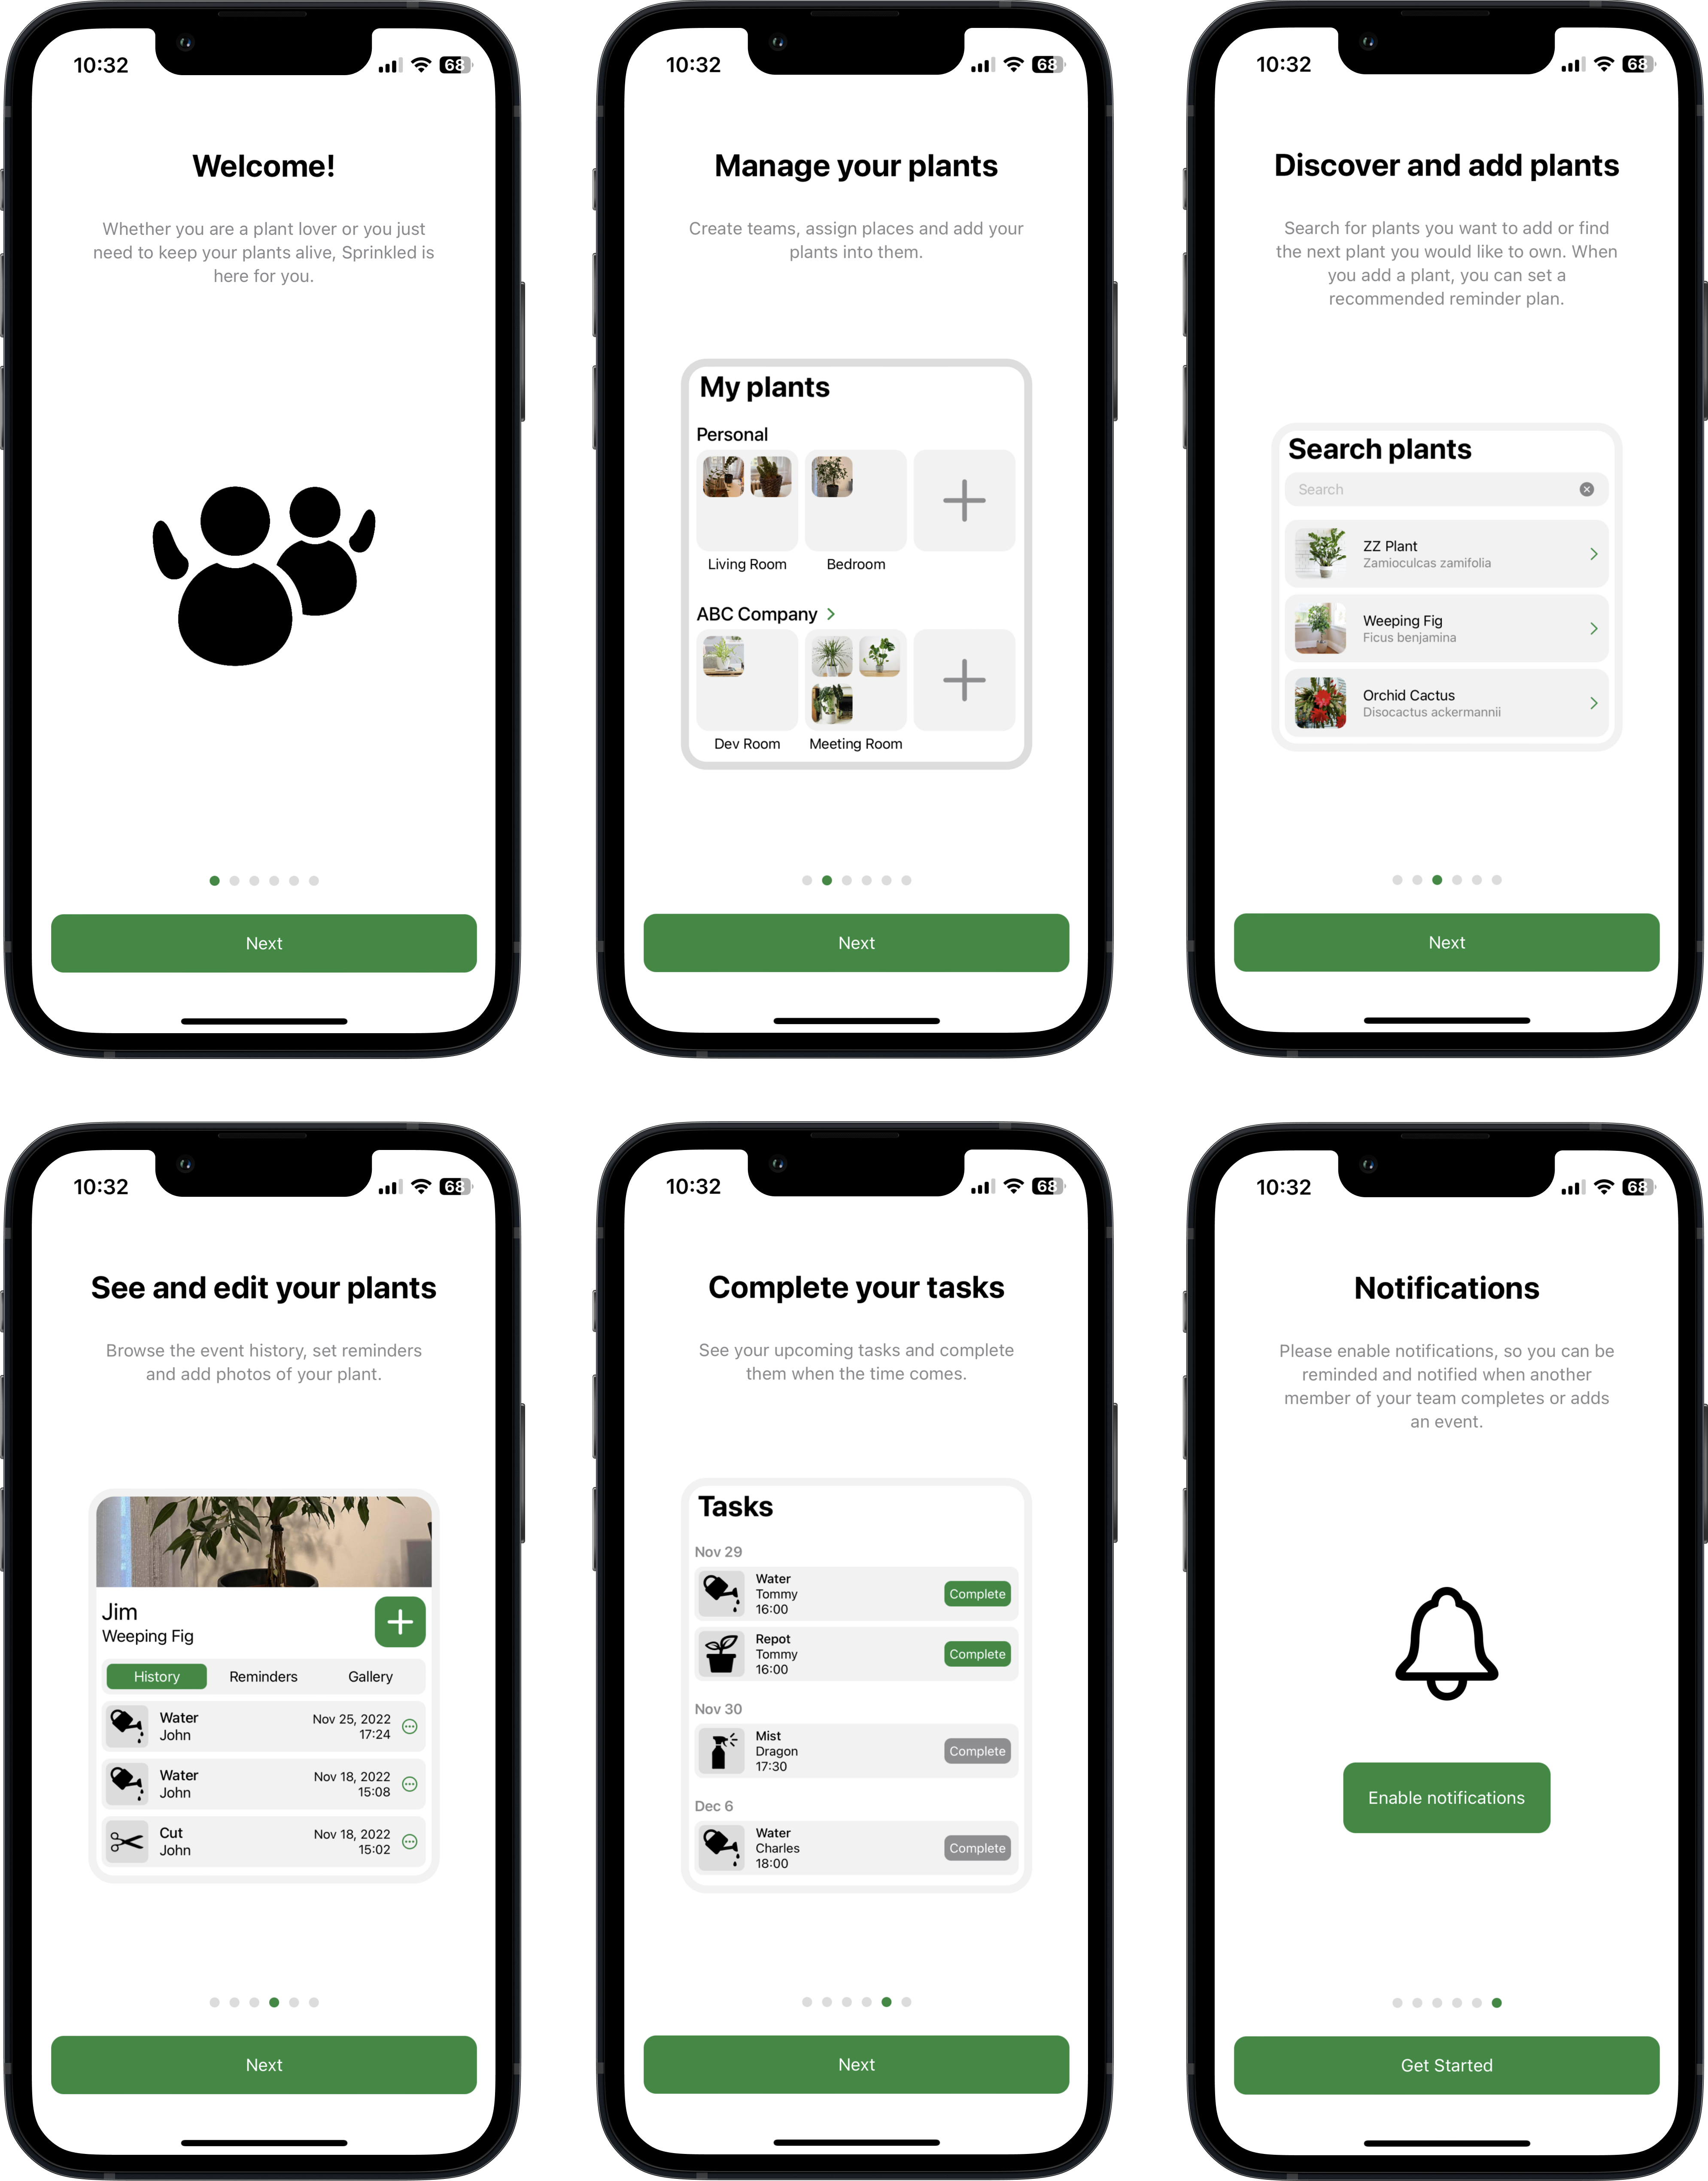
\includegraphics[width=1\linewidth]{images/screenshots-1.png}
  	\caption{Ukázka obrazovek - onboarding}
  	\label{img:screenshots-1}
\end{figure}

\subsection{Správa týmů a míst}
Spravovat týmy a místa může uživatel na obrazovce \uv{My plants}. Ta vypadá téměř identicky jako návrh, změnila se ikonka tlačítka pro vytváření týmů, míst a přidávání rostlin. Je shodné s~tlačítkem pro přidávání na detailu záznamu rostliny.

Do detailu týmu se lze dostat kliknutím na jméno týmu (dostatečným indikátorem, že na něj lze kliknout, by měla být zelená šipka, která se vedle jména týmu nachází). V~detailu týmu může uživatel vidět členy, pokud má práva, může členy přidávat, odebírat nebo jim může dávat/brát práva.

Na obrazovce s~detailem místa se nachází jednotlivé záznamy rostlin (jako dlaždice s~náhledovým obrázkem a názvem), do kterých se může prokliknout. Také zde může místo přejmenovat nebo odstranit.

\begin{figure}
	\centering
	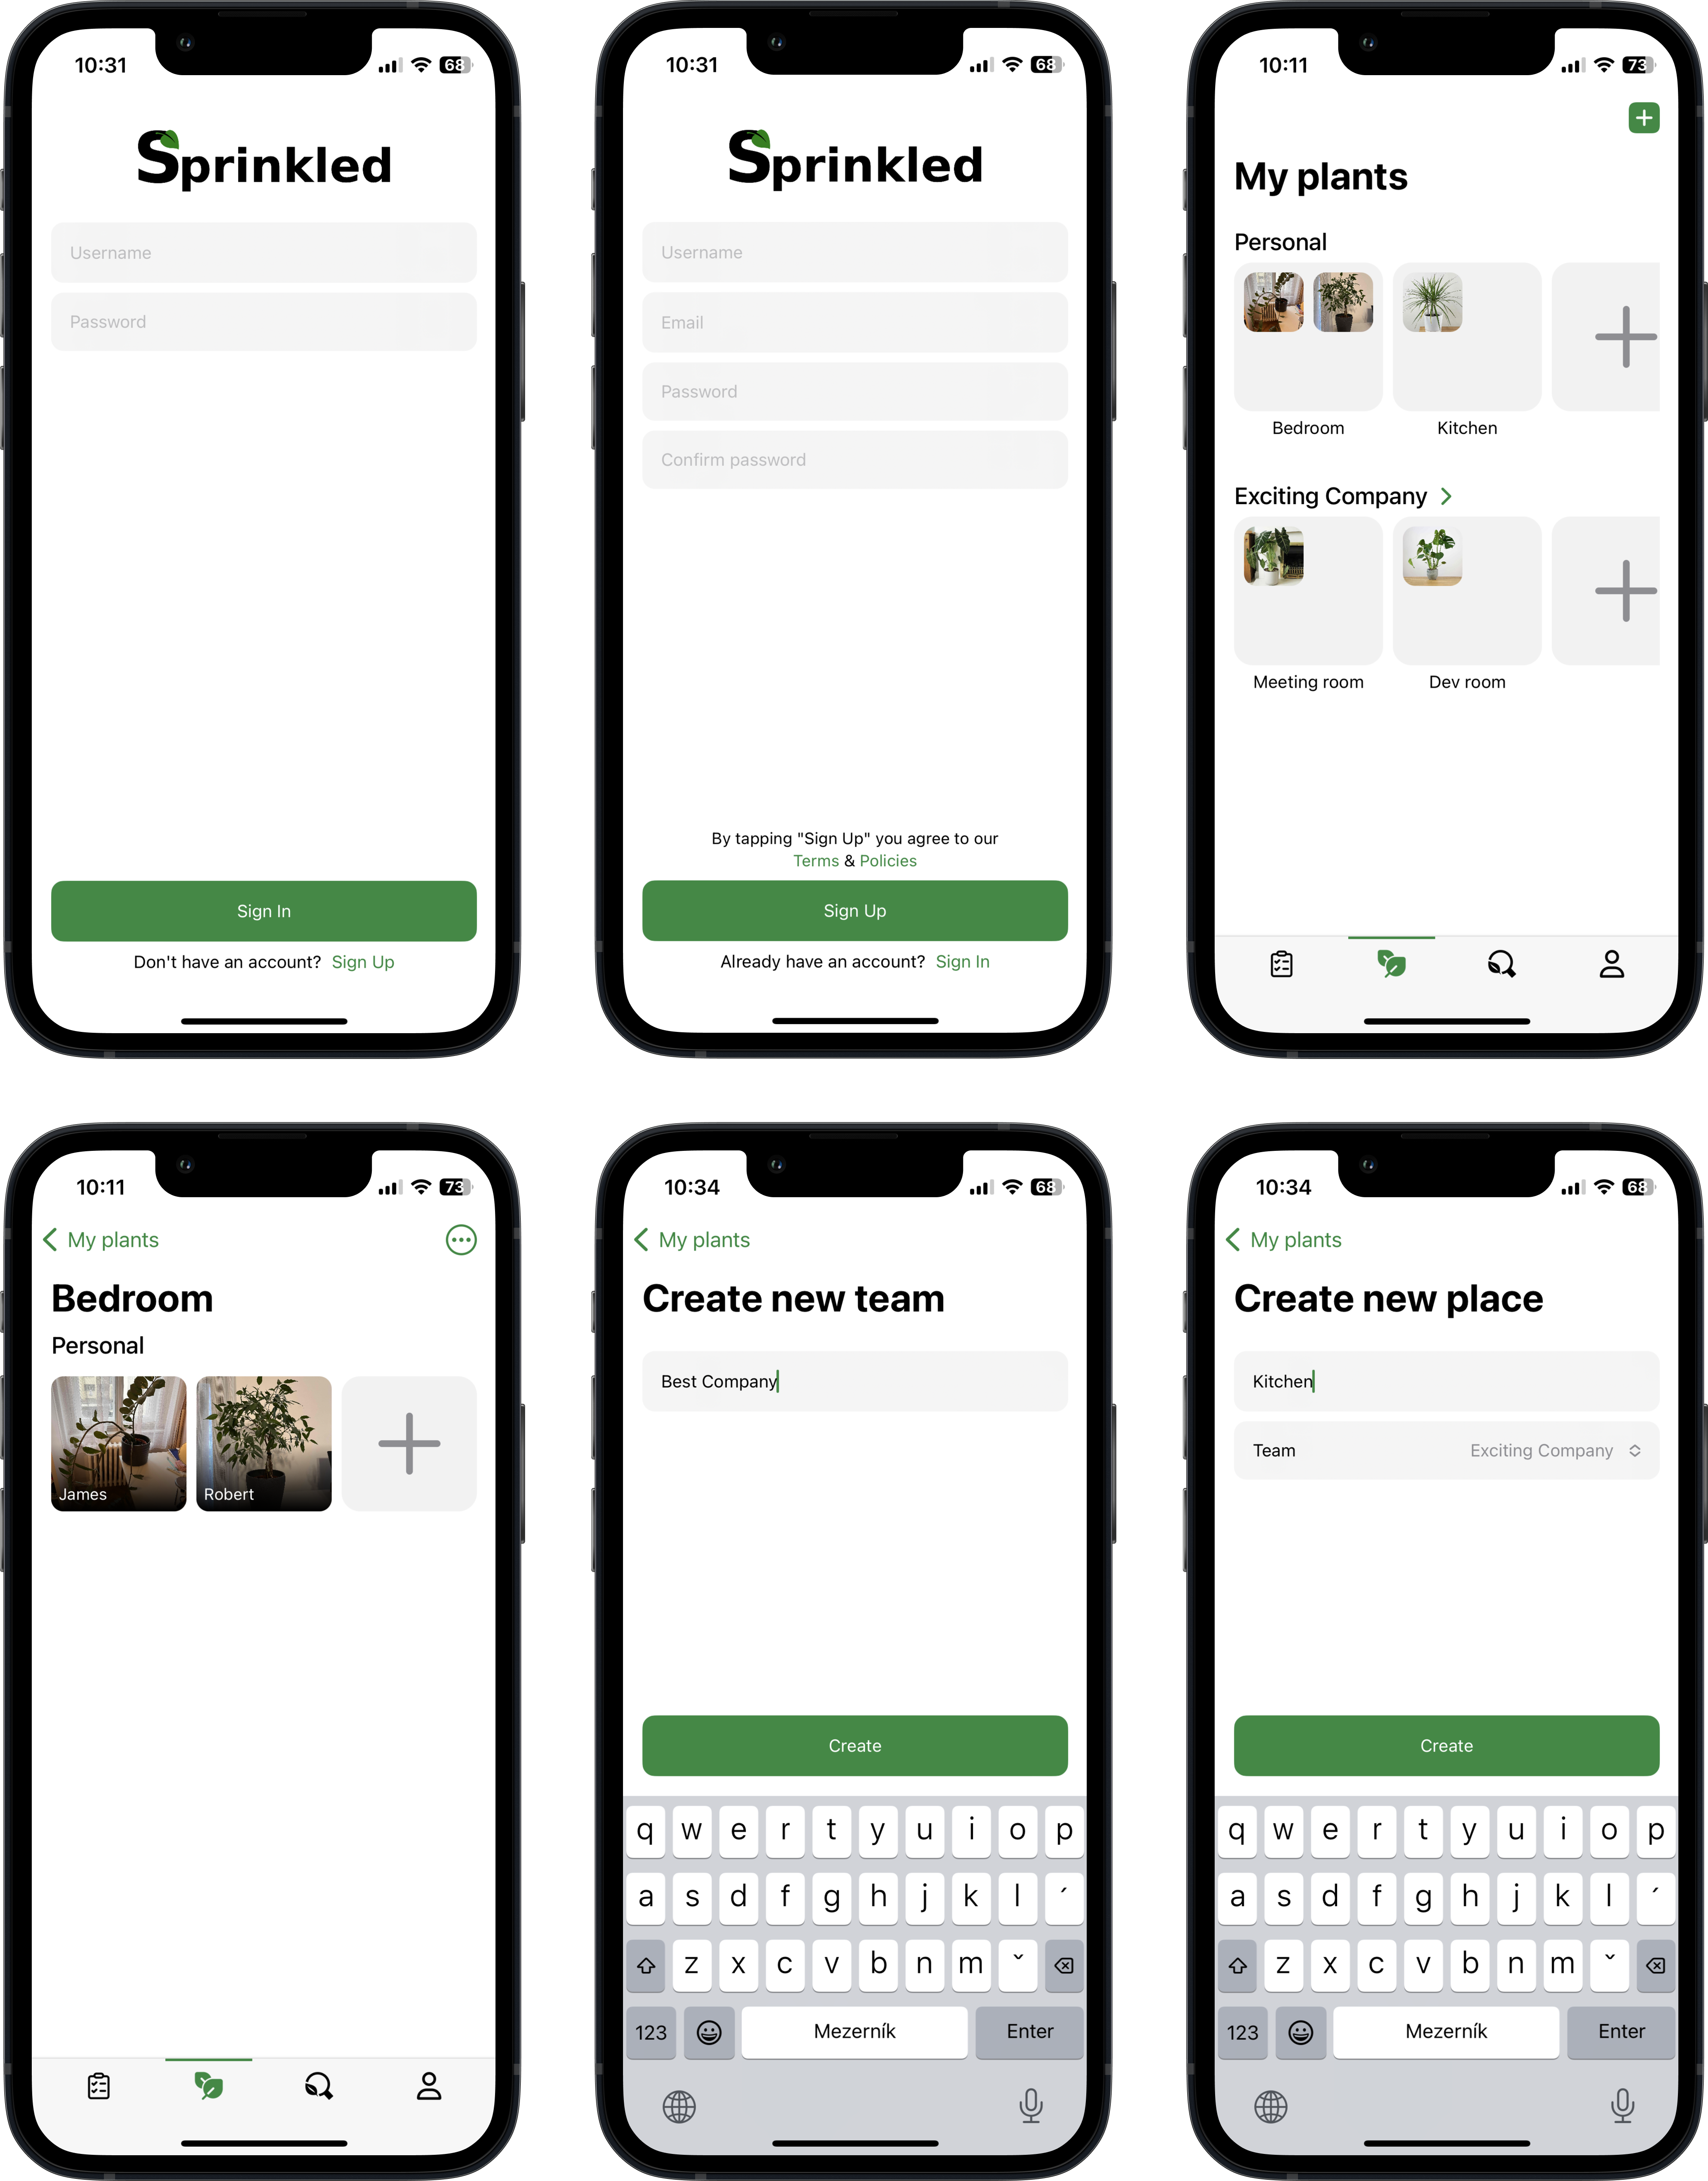
\includegraphics[width=1\linewidth]{images/screenshots-2.png}
  	\caption{Ukázka obrazovek - přihlášení, registrace, moje rostliny}
  	\label{img:screenshots-2}
\end{figure}

\begin{figure}
	\centering
	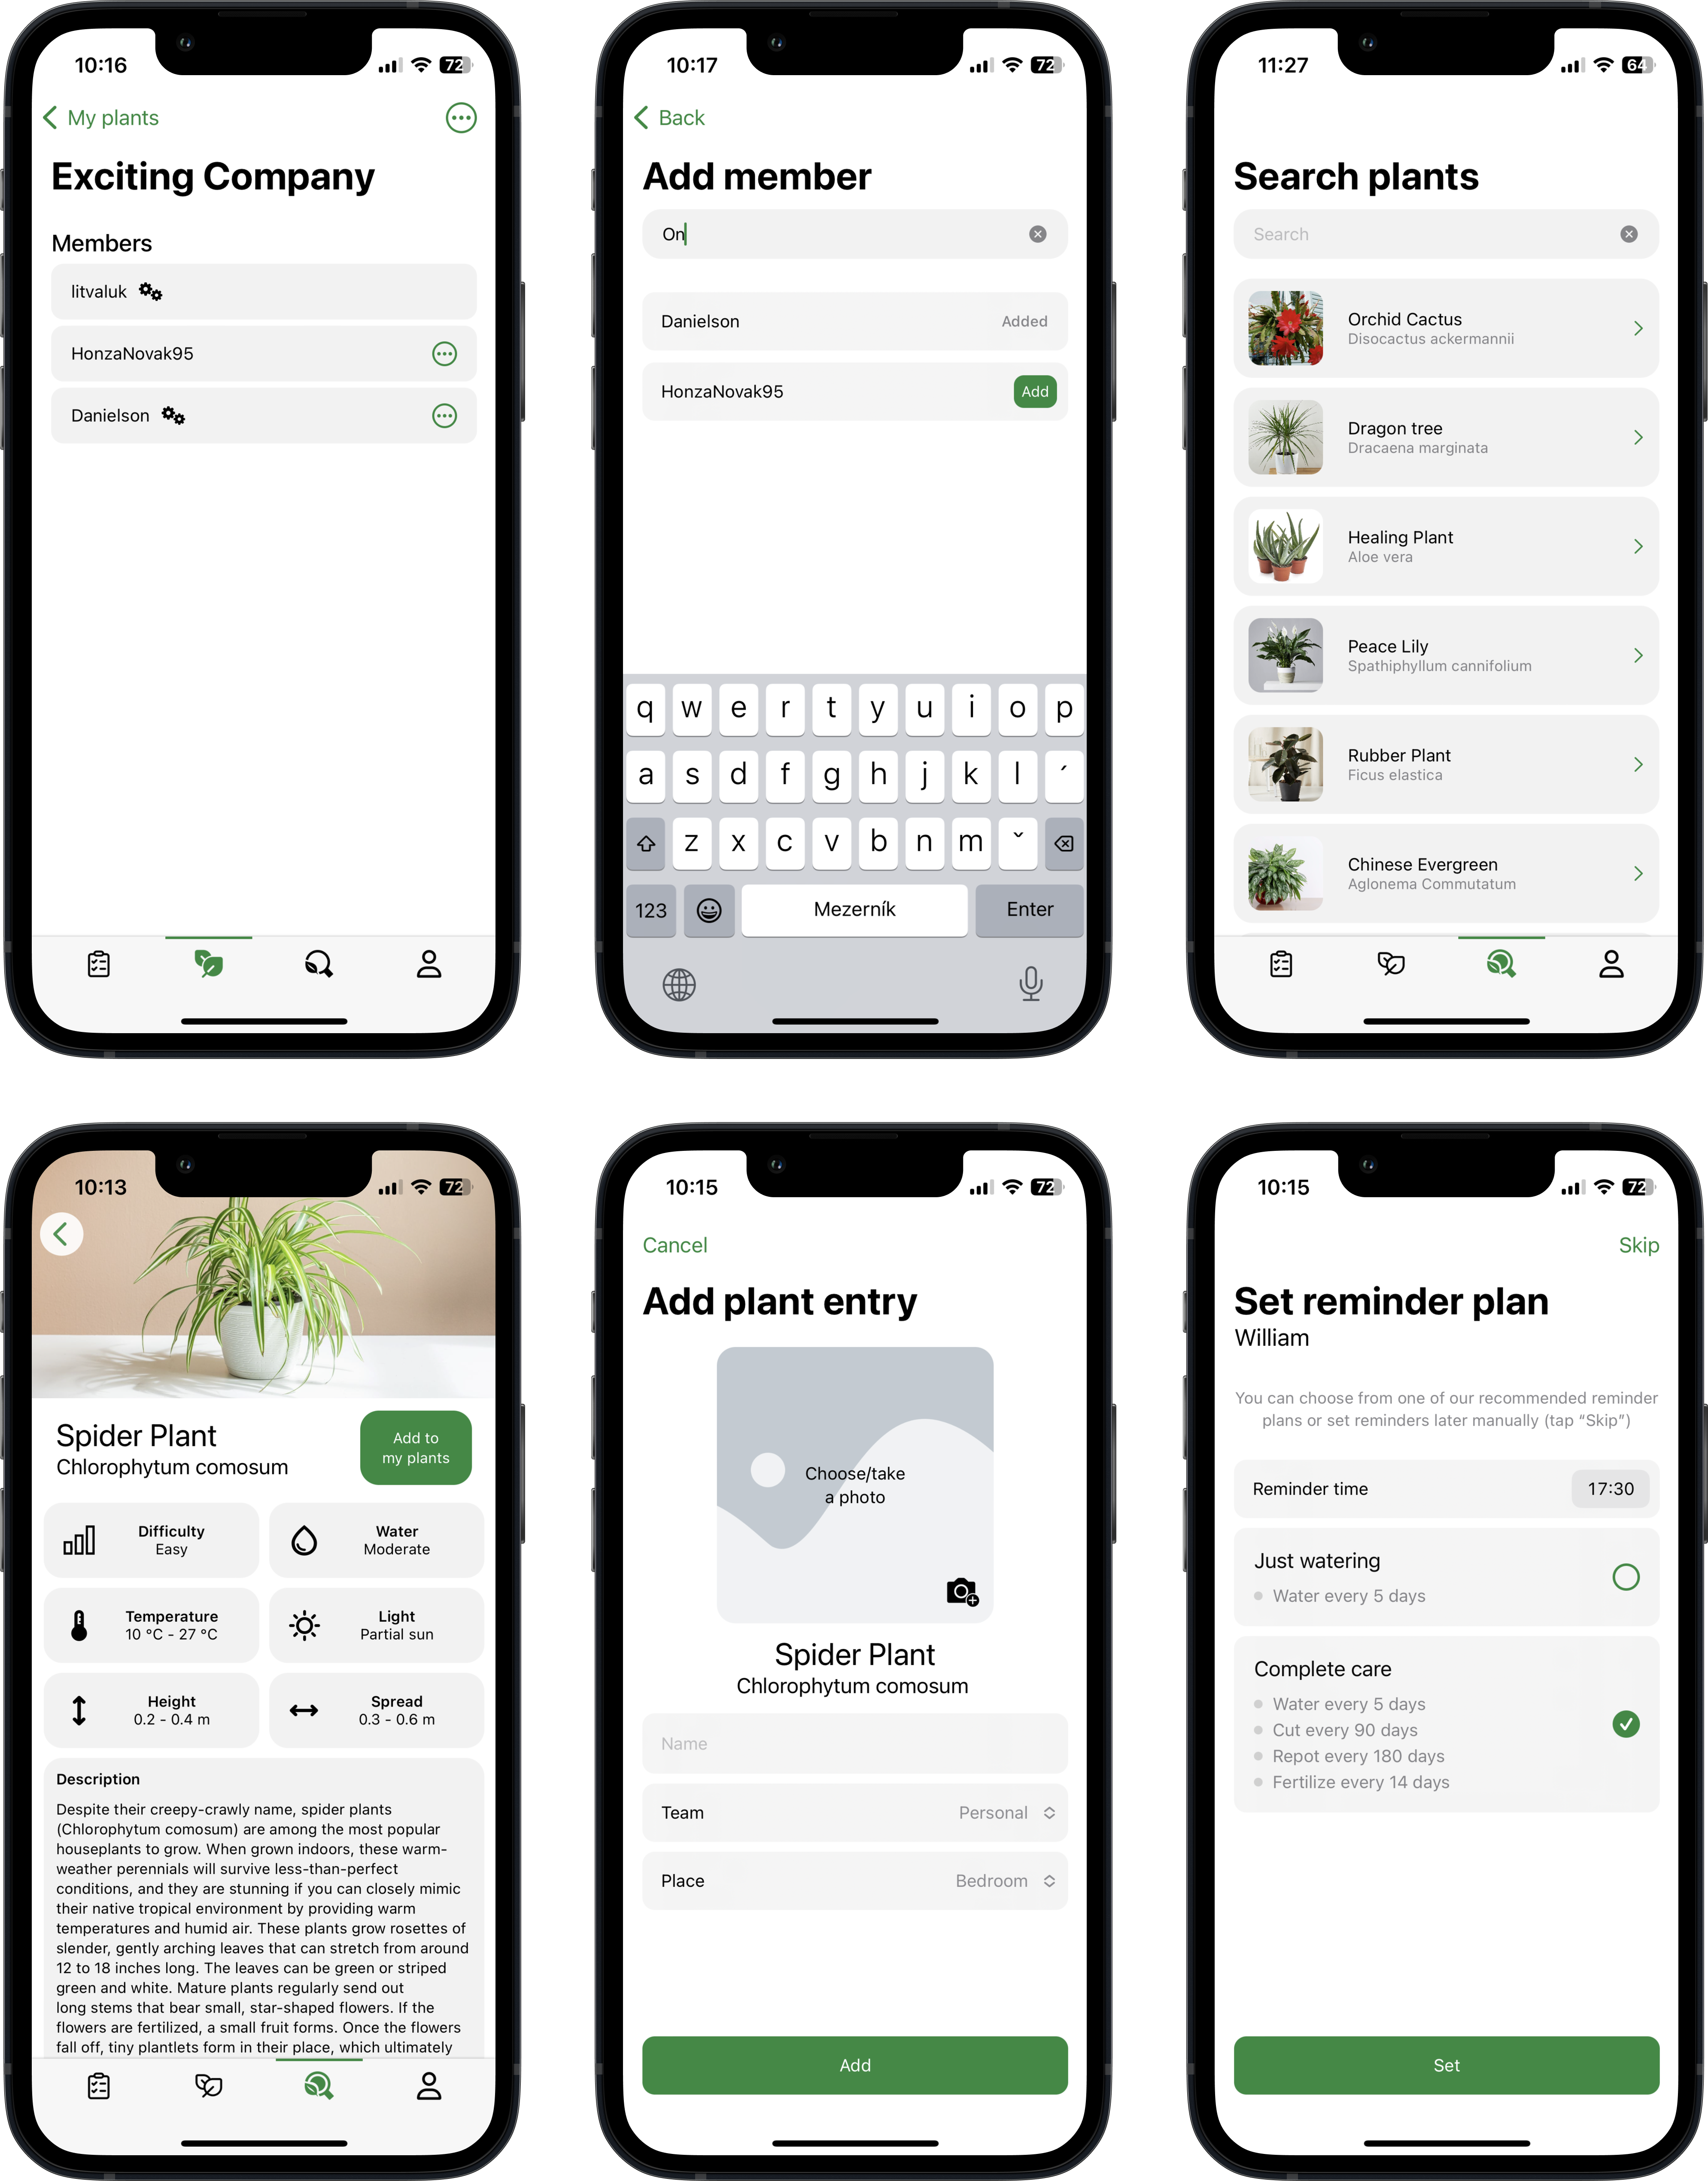
\includegraphics[width=1\linewidth]{images/screenshots-3.png}
  	\caption{Ukázka obrazovek - správa týmu, vyhledávání a přidávání rostliny}
  	\label{img:screenshots-3}
\end{figure}

\subsection{Vyhledávání a přidávání rostlin}
Na obrazovce se seznamem rostlin lze procházet jednotlivé druhy rostlin. Pomocí vyhledávacího pole lze vyhledávat jak podle obecného, tak i latinského názvu. Po kliknutí na jakýkoliv druh rostliny se uživatel dostane do jeho detailu, kde si lze prohlédnout základní informace a může si danou rostlinu přidat do svých rostlin. Na přidávací obrazovce může uživatel nahrát fotografii, specifikovat jméno své rostliny, přiřadit tým a místo. Po přidání rostliny se uživateli zobrazí obrazovka s~nastavením připraveného připomínkového plánu (ten ovšem nastavovat nemusí). Proces vyhledávání a přidávání rostlin je zachycen v~ukázce \ref{img:screenshots-3}.

\subsection{Správa záznamu rostliny}
Z~obrazovky místa se lze dostat na záznamy rostlin, které se v~daném místě nachází. Obrazovka záznamu rostliny vedle obrázku, jména, druhu rostliny a tlačítka pro přidávání událostí, připomínek a fotek obsahuje 3 sekce. Sekci, ve které se uživatel nachází, lze měnit přepínačem (\textit{Picker}). Protože základní přepínač (ve variantě \textit{segmented control}) se nehodil ke vzhledu aplikace, byla vytvořena jeho vlastní implementace.

Seznam událostí a připomínek vypadá obdobně, každá položka obsahuje název akce a příslušnou ikonku. Pod názvem je v~případě události zobrazeno jméno uživatele, který danou událost provedl. U~připomínky je to pak interval, jak často se daná akce má vykonávat (pokud se jedná o~jednorázovou připomínku, je zobrazen popisek \uv{One time}). Na pravé straně položky je poté buď datum a čas provedení události nebo v~případě připomínky její nadcházející spuštění (tedy poslání připomínkové notifikace). Úplně napravo se nachází tlačítko, které vyvolá menu, ve kterém lze událost či připomínku upravit nebo smazat. Upravovací obrazovka je téměř totožná obrazovce přidávací, pouze se mění několik popisků. Před samotným smazáním je uživatel vyzván k~potvrzení akce pomocí vyskakovacího okna.

Galerie se skládá z~dlaždic, obsahující náhledy jednotlivých fotografií. Po rozkliknutí fotografie se uživatel dostane k~detailu fotografie. Zde se nad samotnou fotografií nachází tlačítko pro zavření (také je možné fotografii zavřít jejím potáhnutím pryč) nebo smazání fotografie a pod ní je jméno uživatele (který fotografii přidal) a také datum přidání. Samotnou fotografii lze přiblížit tzv. \textit{magnifying} gestem. Pokud je fotografií více, lze \textit{swipe} gestem mezi nimi procházet.

\begin{figure}
	\centering
	\includegraphics[width=1\linewidth]{images/screenshots-4.png}
  	\caption{Ukázka obrazovek - správa záznamu rostliny}
  	\label{img:screenshots-4}
\end{figure}

\subsection{Úkoly}
Samotné úkoly (řešeny jako nedokončené události) jsou načteny ze serveru do datové struktury \texttt{OrderedDictionary} (z~knihovny Swift Collections). Úkoly jsou tak seskupeny a uloženy pod klíčem, kterým je textový řetězec vyjadřující datum ve formátu \uv{\texttt{MMM d}}. Z~tohoto seřazeného slovníku je v~samotném View vytvořeno seřazené pole (dvojice datum a příslušný seznam událostí), které je následně zobrazeno.

Oproti návrhu se jednotlivé úkoly liší tím, že na pravé straně se nachází tlačítko \uv{Complete}, které po jeho stisknutí označí daný úkol jako dokončený (z~nedokončené události se stane dokončená a ta je zobrazena v~historii příslušné rostliny). Zároveň, pokud se jedná o~úkol, který přísluší týmové rostlině, jsou o~jeho dokončení ostatní členové notifikováni (pokud mají zapnuté notifikace o~událostech).

\subsection{Profil a nastavení}
Obrazovka, ve které uživatel může zapínat nebo vypínat druh notifikací (pomocí prvku \textit{Toggle}), které mu jsou posílány. Dále si také může přepnout měrné jednotky, které se zobrazují v~aplikaci. Může si zde také smazat svůj účet nebo se odhlásit. Ukázka této obrazovky je součástí obrázku \ref{img:screenshots-5}.

\begin{figure}
	\centering
	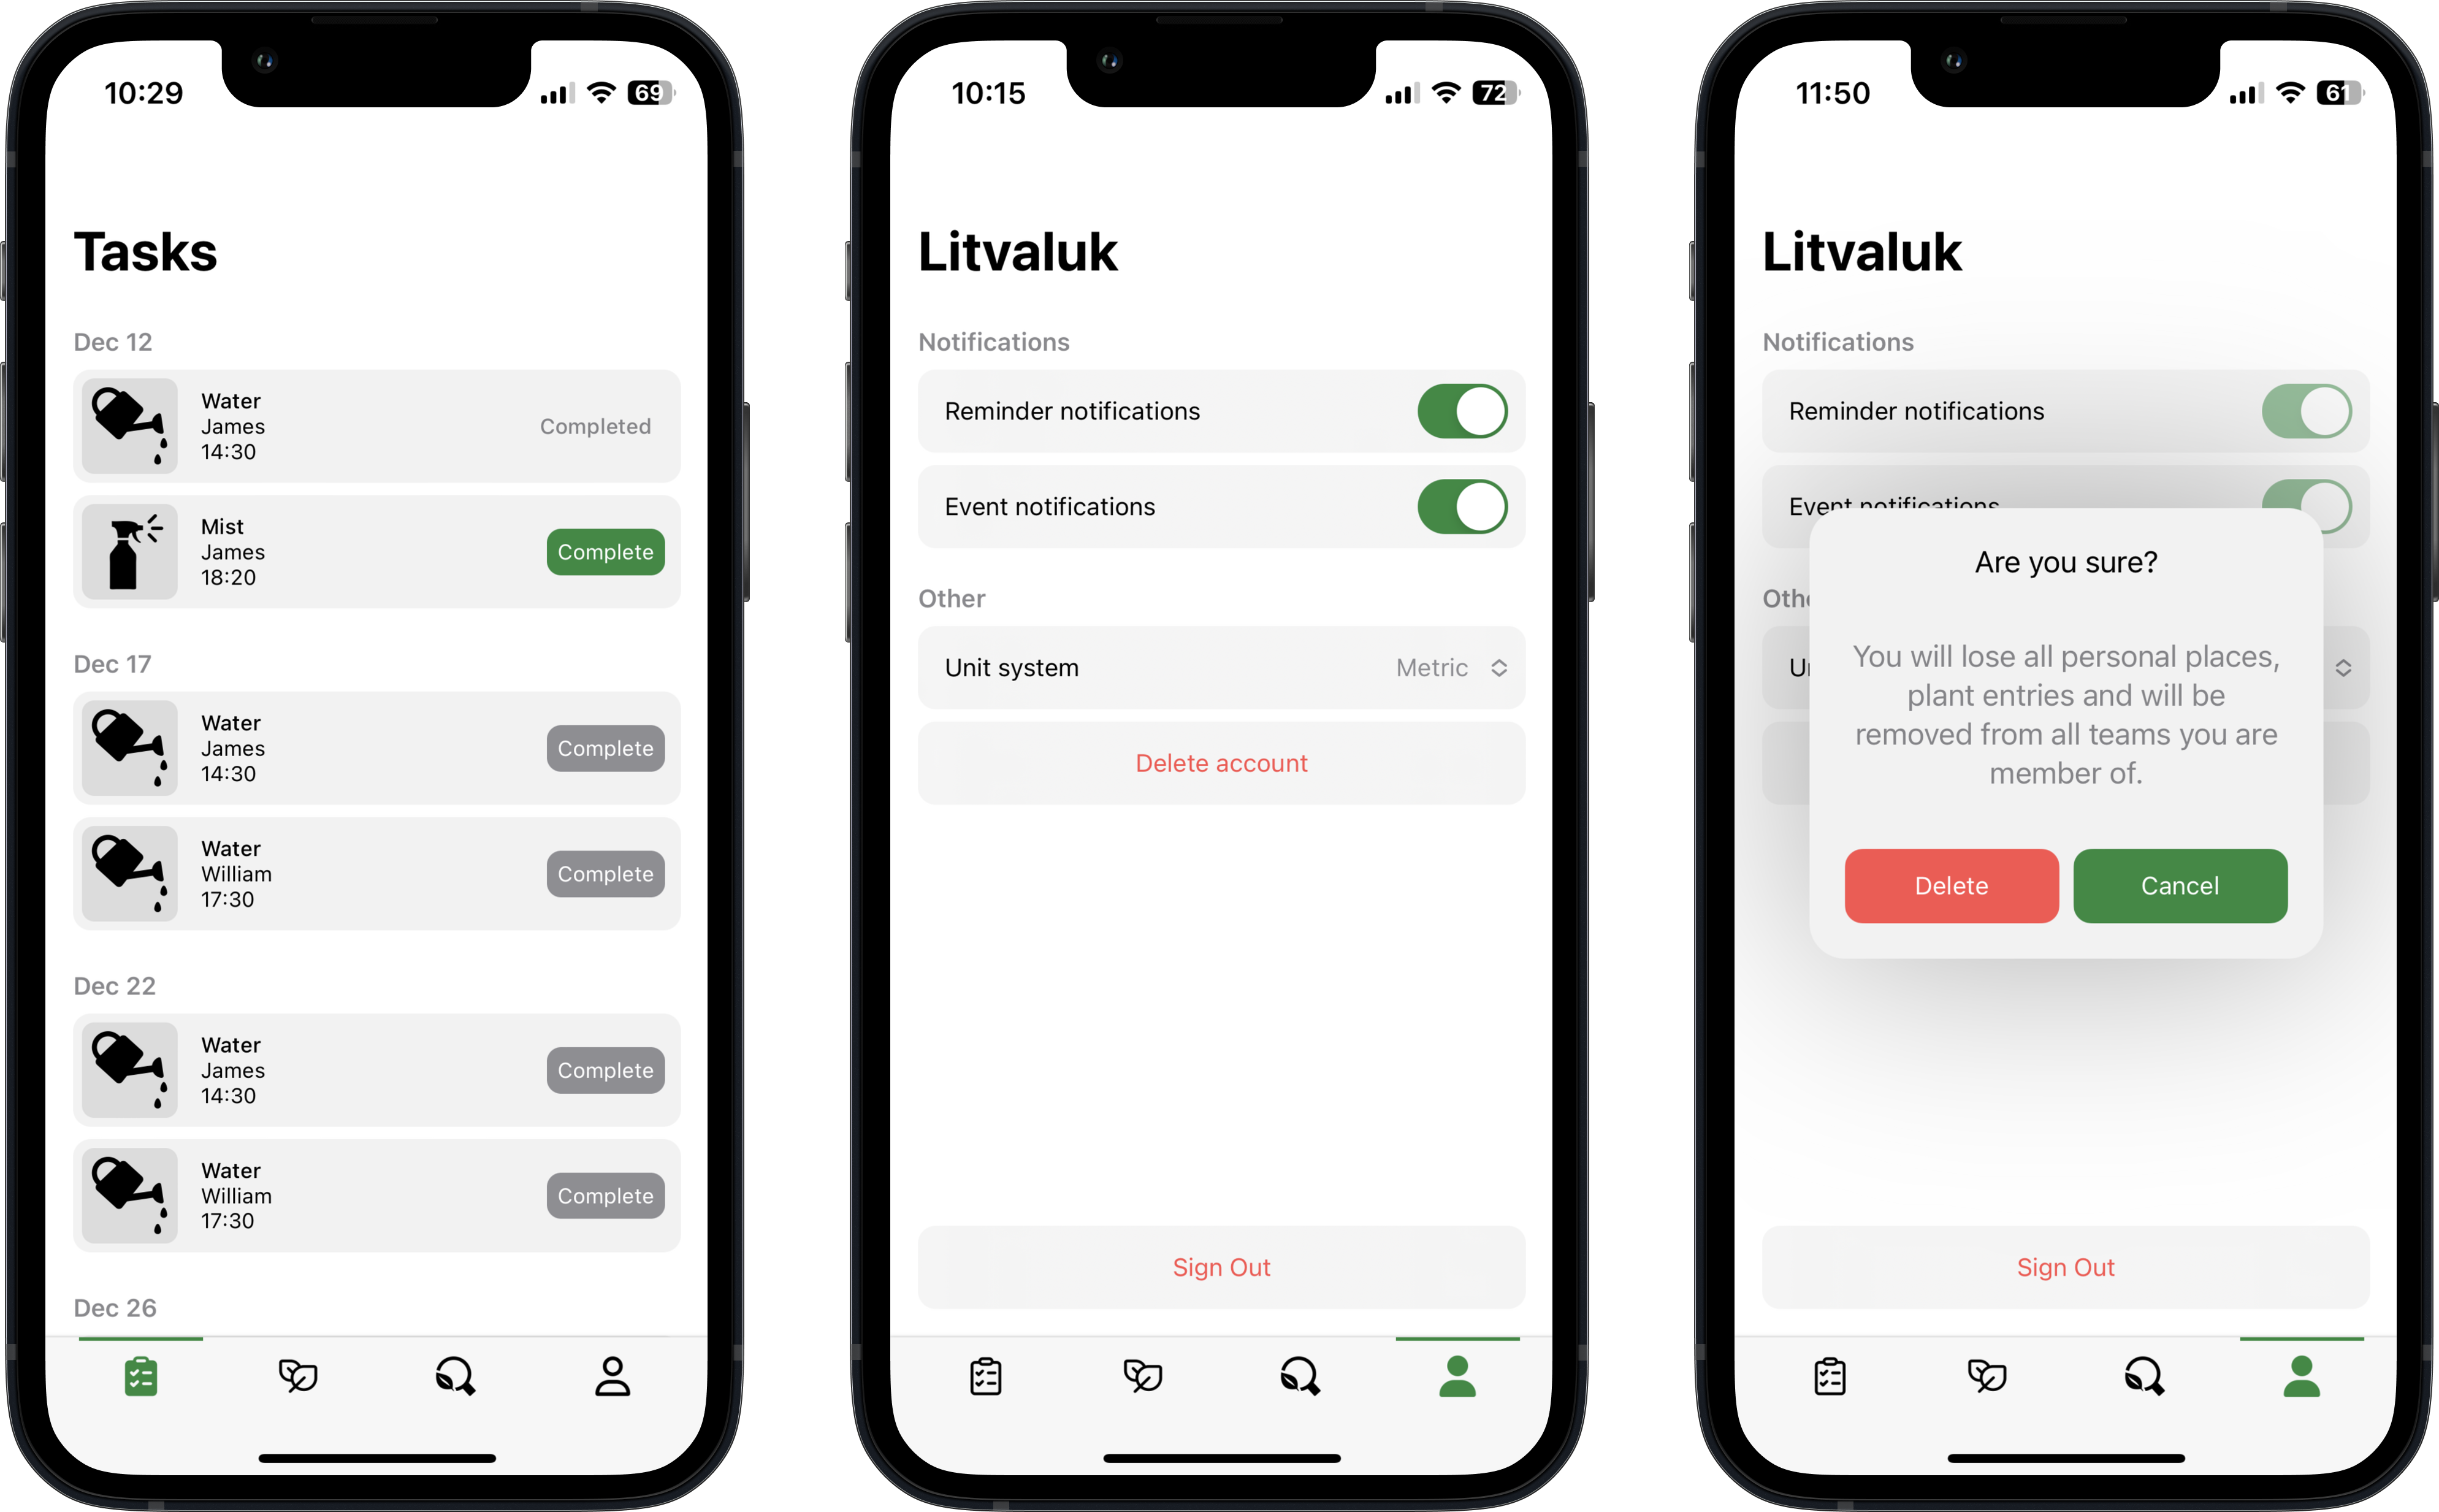
\includegraphics[width=1\linewidth]{images/screenshots-5.png}
  	\caption{Ukázka obrazovek - úkoly a profil/nastavení}
  	\label{img:screenshots-5}
\end{figure}

\subsection{Notifikace}
O~samotné posílání notifikací se stará serverová část, nicméně je potřeba u~každého zařízení získat tzv. \textit{push} token. Pro získání tohoto tokenu je potřeba zavolat metodu \texttt{registerForRemoteNotifications} na singletonu \texttt{UIApplication}. Následně se zavolá v~\texttt{AppDelegate} specifická metoda o~úspěšné registraci \textit{push} notifikací, ve které se push token nachází v~parametru dané metody. Tento token je poté odeslán na server a uložen v~databázi.

Na jednotlivá zařízení tedy chodí 2 druhy notifikací:

\begin{description}
    \item[Událostní] Tuto notifikaci obdrží ta zařízení, na kterých je právě přihlášený uživatel (zároveň má povolené událostní notifikace), jež se nachází v~týmu, ve kterém právě někdo přidal událost nebo dokončil úkol u~některé z~rostlin. Obsahuje uživatele, o~jakou akci se jedná a na jaké rostlině byla provedena.
    \item[Připomínkové] Je poslána v~okamžik, kdy aktuální čas odpovídá času některé z~připomínek. Je poslána na zařízení všech příslušných uživatelů, kteří mají povolené připomínkové notifikace.
\end{description}

\subsection{Tmavý režim}
Protože operační systém iOS od verze 13 podporuje tmavý režim, je zvykem, že aplikace tento režim podporují. V~případě aplikace \uv{Sprinkled} tomu není jinak. Implementačně se nejedná a složitý úkon, v~projektu je potřeba definovat jednotlivé barvy, které aplikace používá v~rámci \textit{Assets} (prostředky). Každé barvě je poté přidána světlá a tmavá varianta. Aplikace už pak mezi těmito barvy dokáže podle zvoleného režimu přepínat. Ukázku tří obrazovek ve tmavém režimu lze vidět na obrázku \ref{img:screenshots-dark-mode}.

\begin{figure}[H]
	\centering
	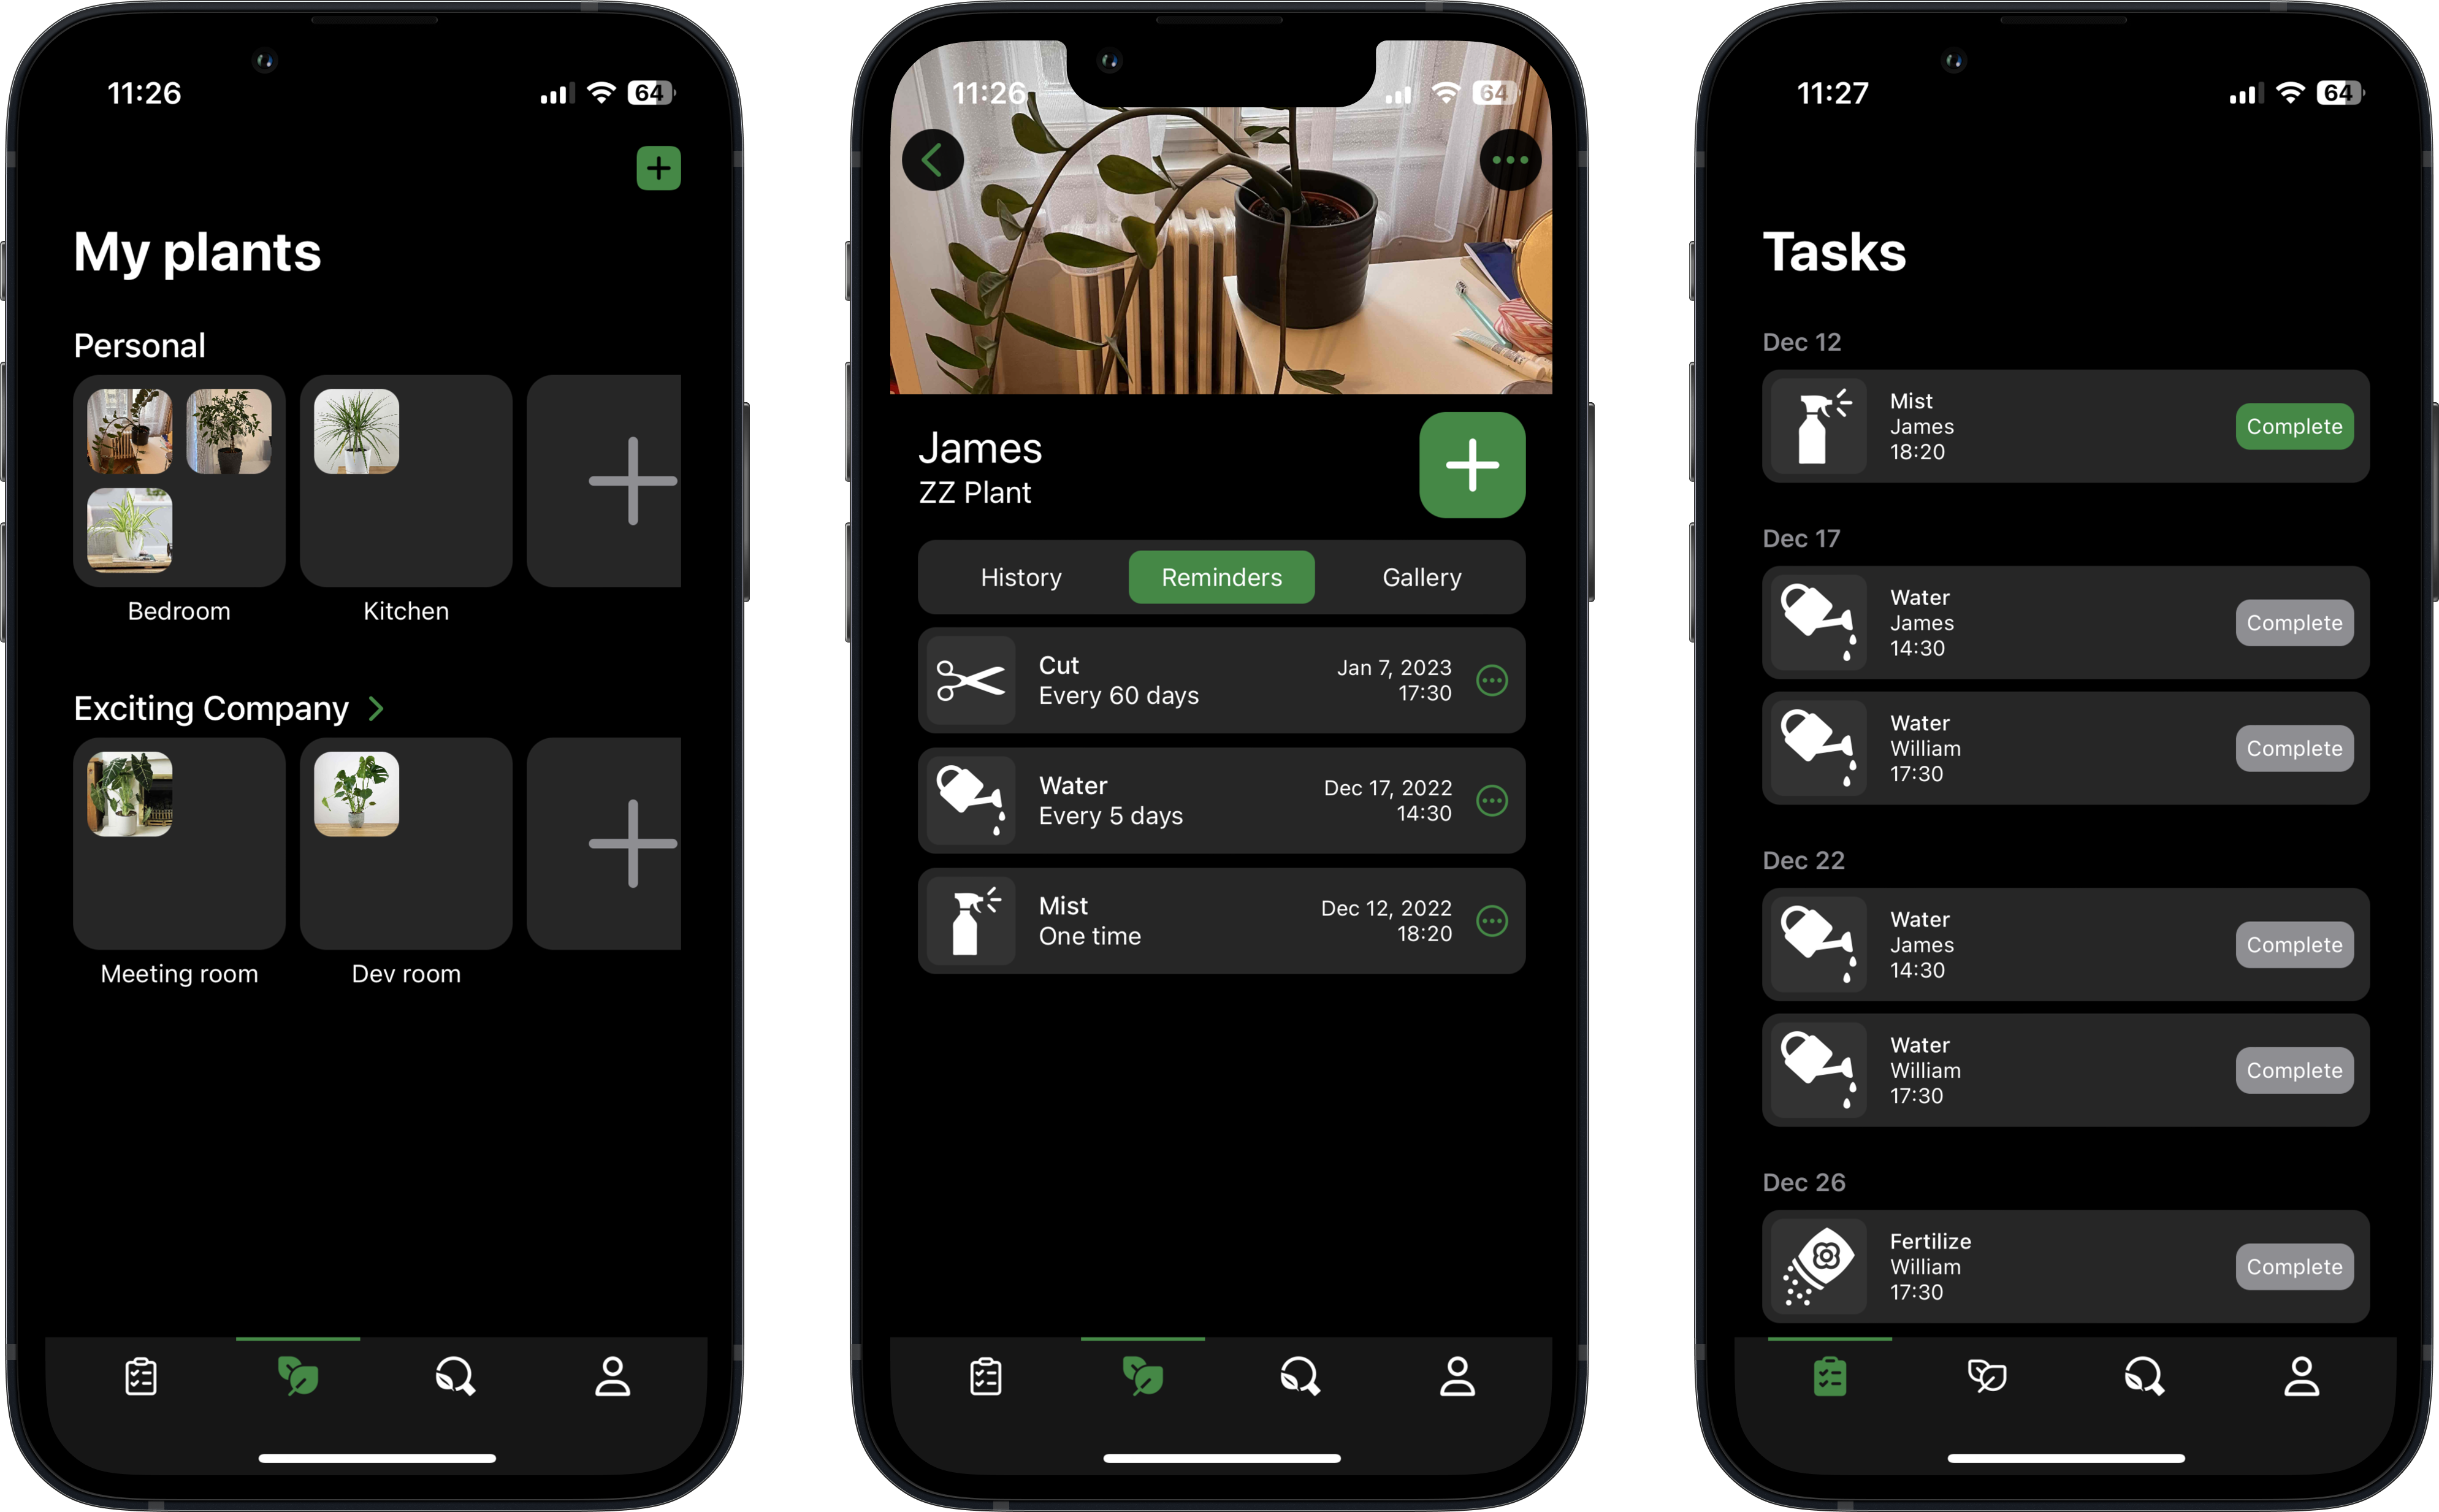
\includegraphics[width=1\linewidth]{images/screenshots-dark-mode.png}
  	\caption{Ukázka obrazovek v~tmavém režimu (dark mode)}
  	\label{img:screenshots-dark-mode}
\end{figure}

\subsection{Zveřejnění aplikace}
Pro nahrání a zveřejnění aplikace na App Store bylo potřeba zřídit si Apple účet s~aktivním vývojářským programem (Apple Developer Program). Ten je pro jednotlivce zpoplatněn sumou 99 dolarů ročně. V~nástroji App Store Connect, který slouží pro správu aplikací v~App Store, byla vytvořen záznam o~aplikaci s~názvem \uv{Sprinkled}. Pomocí XCode byl z~implementace aplikace vytvořen archiv, který byl na App Store Connect nahrán. V~tomto stavu bylo možné aplikaci interně testovat v~aplikaci TestFlight, aniž by bylo potřebné podstupovat jakýkoliv schvalovací proces.

Pro zpřístupnění aplikace veřejnosti bylo potřeba vyplnit popis, klíčová slova, informace o~využívání citlivých dat, poskytnout data o~dostupnosti, nahrát náhledové fotografie (viz \ref{img:appstore-preview}), nastavit věková omezení a cenu (aplikace je dostupná zadarmo). Také bylo ještě potřeba v~aplikaci vytvořit účet a vyplnit tyto přihlašovací údaje, aby aplikaci mohl pracovník z~Apple vyzkoušet a schválit.

Aplikace byla jednou vrácena z~důvodu neposkytnutí možnosti smazání účtu. Apple totiž ve své směrnici (App Store Review Guidelines) vyžaduje, aby aplikace, které umožňují vytváření účtů, zároveň také poskytly možnost pro mazání účtů. Tato funkcionalita byla tedy do aplikace dodělána a následně aplikace schvalovacím procesem prošla. Aplikace je dostupná v~App Store na \cite{sprinkled-appstore}.

\begin{figure}
	\centering
	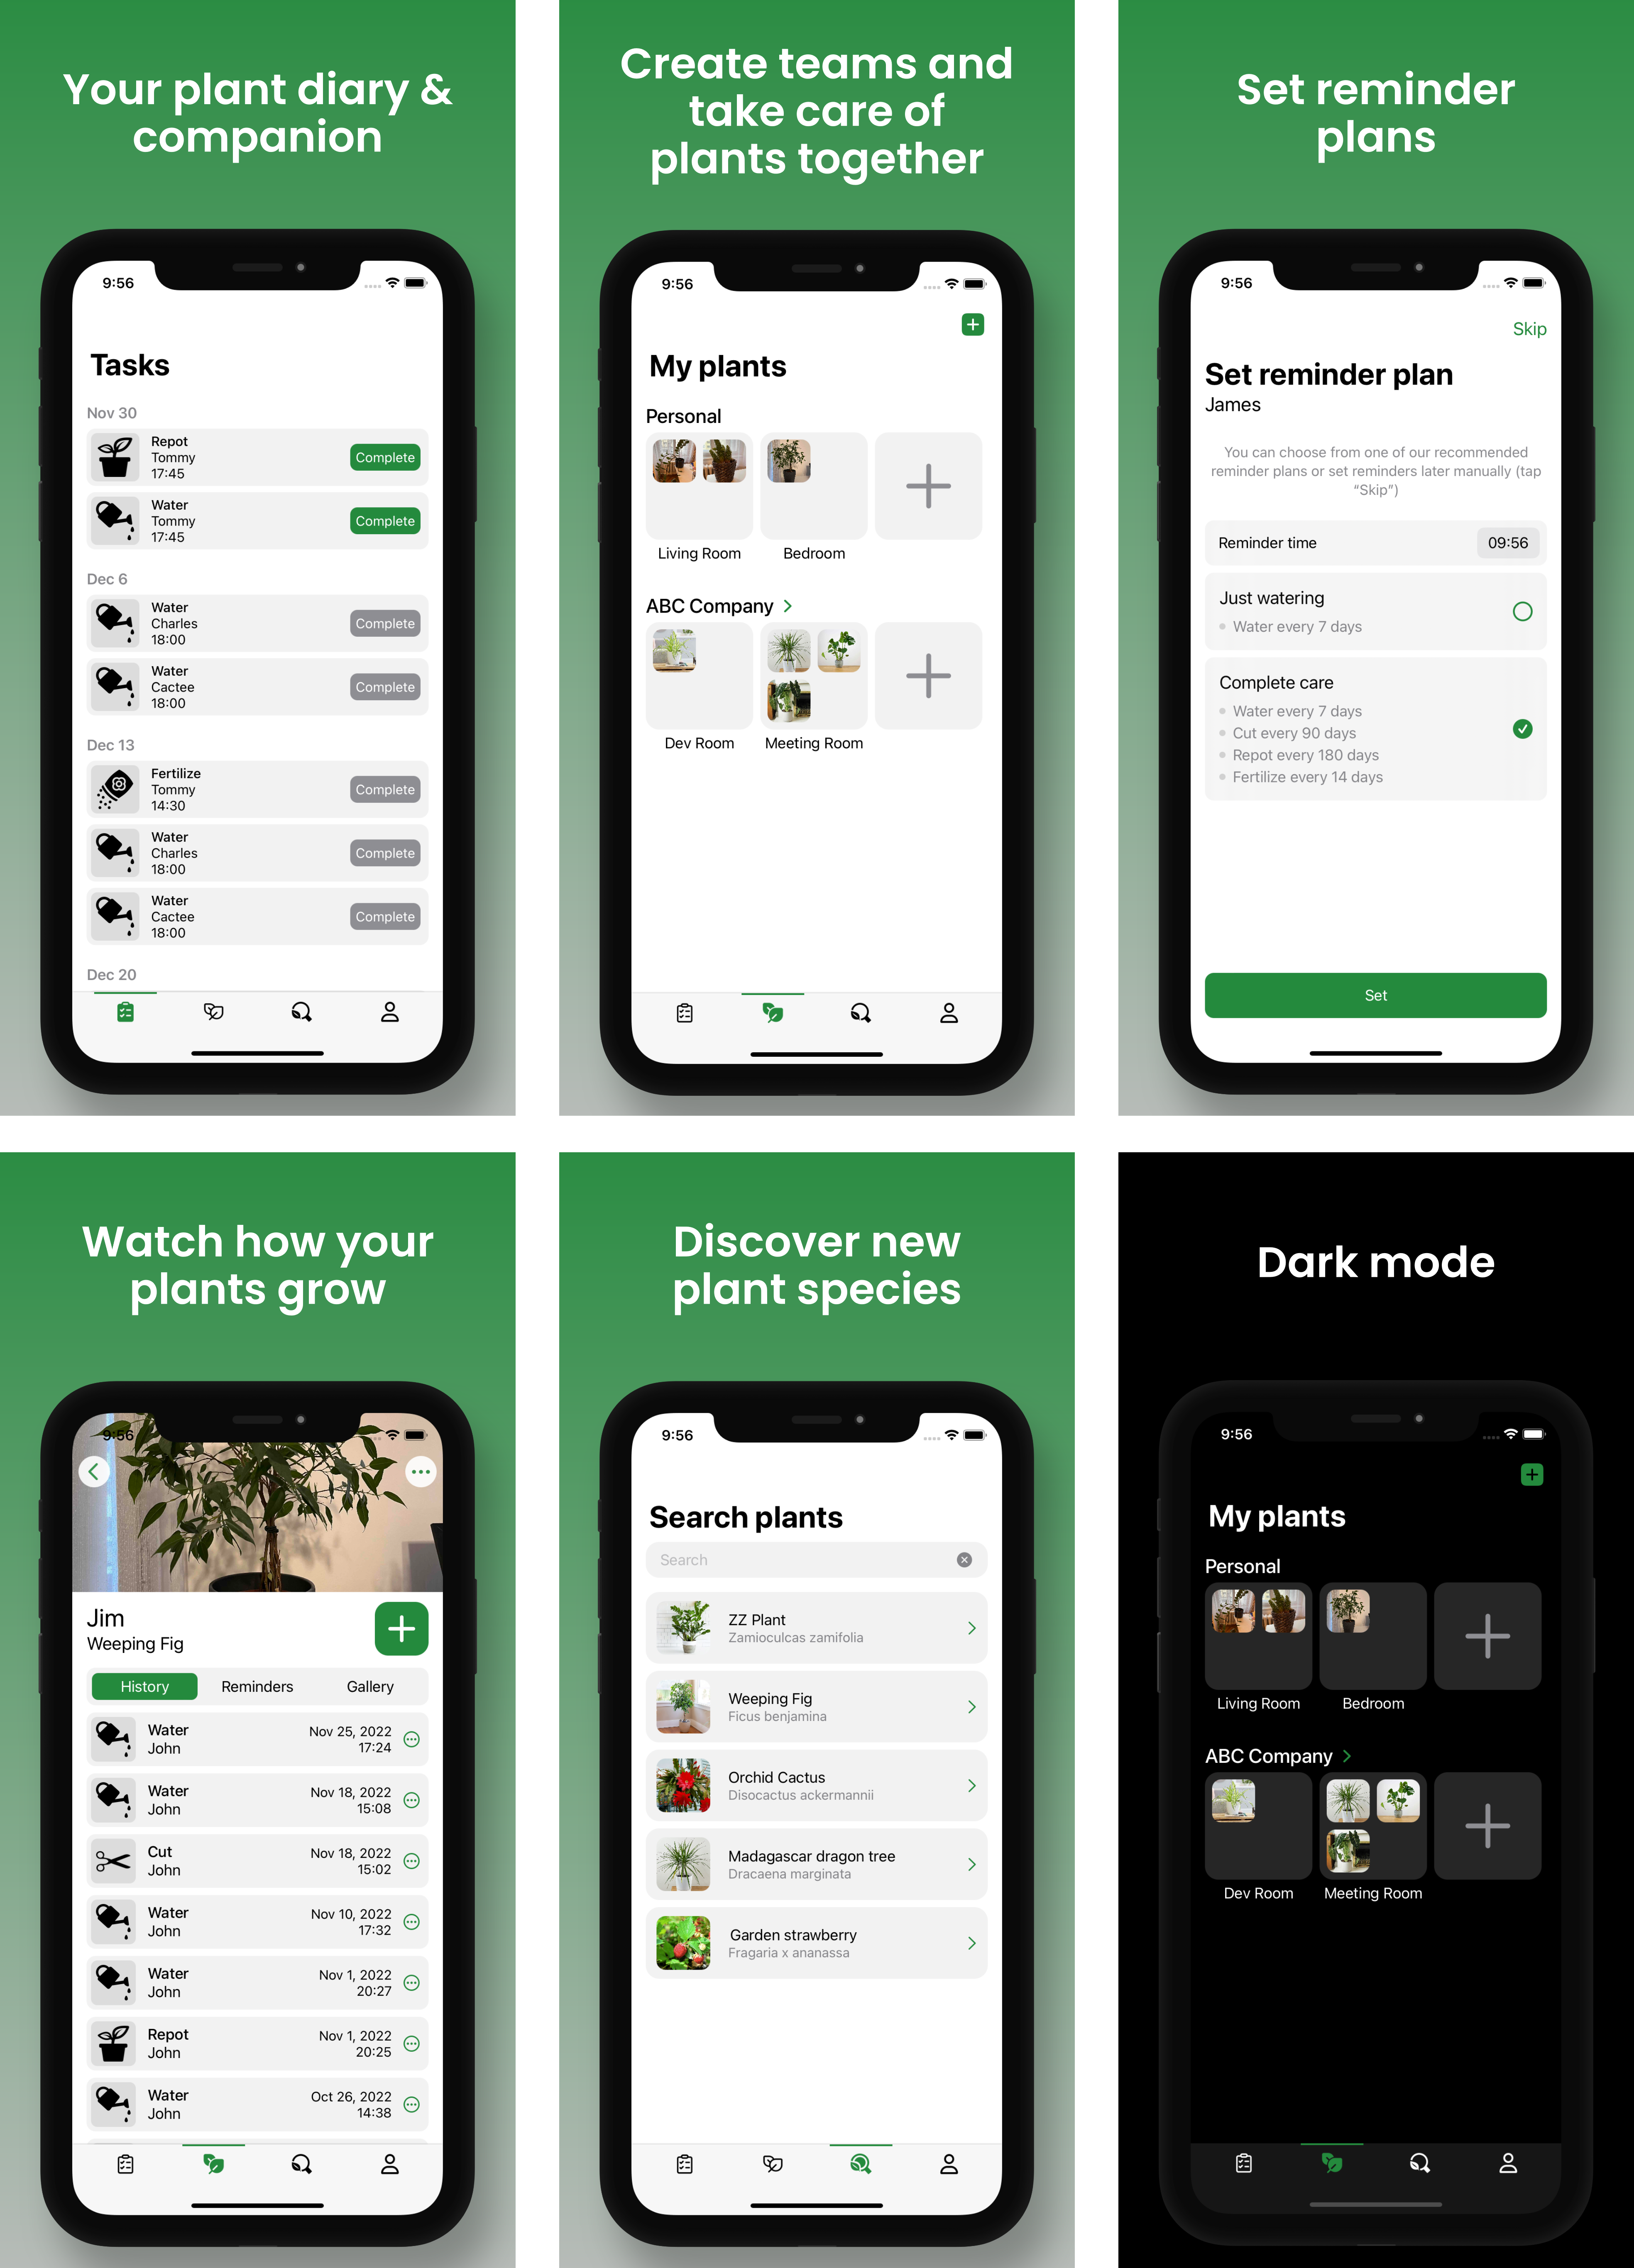
\includegraphics[width=1\linewidth]{images/appstore-preview.png}
  	\caption{Náhledové obrazovky v~App Store}
  	\label{img:appstore-preview}
\end{figure}

% --------------------------------------------------------------------------------------------

\chapter{Uživatelské testování}
Tato kapitola se věnuje uživatelskému testování. Uživatelské testování (také známe jako \textit{Usability Testing}) je jednou z~oblíbených metod testování UX. Malá skupina uživatelů (z~cílové skupiny) plní úkoly v~rámci aplikace, zatímco moderátor pozoruje jejich chování a dělá si poznámky. Cílem tohoto testování je zjistit, zda jsou uživatelé, kteří aplikaci vidí poprvé, schopni se zorientovat a provést zadané úkoly. Tímto lze odhalit problémy v~návrhu uživatelského rozhraní a ty případně opravit.

Předpokladem bylo zvolit testery, kteří jsou aktivními uživateli mobilních zařízení s~operačním systémem iOS. Tím bylo zaručené, že umí zařízení používat a zároveň mohou aplikaci otestovat na vlastním zařízení. Zároveň také musí umět anglicky, neboť aplikace podporuje (prozatím) pouze angličtinu. Bylo vybráno celkem 5 (doporučený počet dle \cite{number-of-testers}) účastníků, kteří spadají mezi typické a příležitostné uživatele. Testování proběhlo na již nasazené a vydané aplikaci. A~bylo rozděleno na tři části.

\begin{description}
    \item[Pre-test] Seznámení testerů s~testovacím procesem, krátké popsání aplikace a optání se na několik otázek, které se týkají jejich vztahu k~rostlinám, jestli nějaké vlastní a starají se o~ně a případně jestli používají, či zkusili použít nějakou aplikaci pro péči o~rostliny.  Následně byly podány instrukce k~nainstalování aplikace z~obchodu s~aplikacemi \textit{App Store}.
    \item[Testovací scénáře] Samotné testování aplikace, bylo rozděleno do 11 scénářů, které na sebe navazují.
    \item[Post-test] Zadání několika otázek, které zjišťují celkové pocity testerů z~aplikace, co se jim líbilo/nelíbilo, jejich nápady na zlepšení a zda by aplikaci využili.
\end{description}

U~každého testování byla zaznamenávána obrazovka zařízení a zvuk z~externího mikrofonu. Jednotlivé nahrávky se nachází na přiloženém médiu.

\section{Pre-test}
Nejdříve byli testeři požádáni, aby se představili. Jednalo se o~dvě ženy a tři muže ve věkovém rozpětí 24 až 25 let. Jeden muž a žena byli čerstvě vystudovaní zubaři a zbytek studenti architektury. Poté
jim byly položeny následující otázky:
\begin{itemize}
    \item Vlastníte a staráte se (nyní nebo v~minulosti) o~nějaké rostliny?
    \item Jakým způsobem jste se o~ně staral/a? Co všechno jste musel/a dělat?
    \item Vyzkoušel/a jste či používáte nějakou mobilní aplikaci, která vám pomáhá se starat o~rostliny?
\end{itemize}
Všichni až na jednoho sdělili, že aktuálně vlastní a starají se o~2 nebo více rostlin. Povětšinou se jedná o~nenáročné rostliny, které intuitivně zalévají. Dva testeři navíc rostliny občas zastřihávají, přesazují nebo otáčejí za sluncem. Žádný y testerů nevyužil specializovanou aplikaci, která by pomáhala se staráním o~rostliny. Jeden vyzkoušel v~historii použít klasické připomínky (základní aplikace), nicméně tento postup se neosvědčil.

Poté jim bylo vysvětleno, jak si mají aplikaci stáhnout a nainstalovat, načež u~každého vše proběhlo bez problémů.

\section{Testovací scénáře}
Testerům byly postupně předkládány kartičky se zadáním jednotlivých testovacích scénářů. Tyto scénáře jsou zkonstruovány tak, aby byly splnitelné samostatně bez doptávání. Zásah moderátora a poskytnutí pomoci by totiž znamenalo, že aplikace nefunguje zcela správně nebo je část uživatelského rozhraní špatně navržená.

\subsection{Registrace}
Tento scénář je zaměřen na prvotní spuštění aplikace a následné vytvoření nového uživatele. Po úspěšné registraci se novému uživateli zobrazí onboarding. U~onboardingu je nutné sledovat, zda si ho testeři opravdu čtou, či ho rovnou přeskočí. K~provedení tohoto scénáře není potřeba žádného předpokladu.
\subsubsection*{Zadání}
Otevřete aplikaci, vytvořte si nový účet a dostaňte se na obrazovku \uv{My plants}. Registrujte se pod uživatelským jménem \textit{Franta01} a použijte email \textit{franta01@gmail.com}. Heslo zvolte libovolné.
\subsubsection*{Očekávaný průchod}
\begin{enumerate}
    \item Otevření aplikace
    \item Kliknutí na klikatelný text \uv{Sign Up}
    \item Zadání informací potřebných k~registraci
    \item Kliknutí na zelené tlačítko \uv{Sign Up}
    \item Prohlédnutí onboardingu
    \item Zavření onboardingu
\end{enumerate}
\subsubsection*{Vyhodnocení}
S~tímto scénářem nebyl víceméně žádný problém, pouze v~jednom případě tester zadával registrační údaje jako přihlašovací, načež pak zjistil, že se nejdříve musí do registrační obrazovky prokliknout. Vhodným řešením by mohlo být zobrazení registrační obrazovky jako první obrazovky při otevření aplikace. Zároveň registrace bude zřejmě častějším úkonem než přihlášení. Všichni si po registraci pečlivě prošli onboarding a pouze 2 si povolili notifikace.
\subsection{Přidání rostliny}
V~tomto scénáři by měl být testovací subjekt sám schopný přidat rostlinu do seznamu svých rostlin. To se může zprvu zdát jednoduché, ale cesta, jak se k~výsledku dostat, nemusí být úplně přímočará. Subjekt se musí co nejrychleji zorientovat v~rozhraní (měl by už mít ponětí, co lze v~aplikaci dělat, pokud si prohlédl onboarding), přidat místo a do něj vytvořit záznam o~rostlině. Předpokladem pro splnění je již přihlášený uživatel.
\subsubsection*{Zadání}
Doma v~obývacím pokoji máte fíkus (obecný anglický název Weeping Fig, latinsky Ficus benjamina). Přidejte ho tedy do svých rostlin.
\subsubsection*{Očekávaný průchod}
\begin{enumerate}
    \item Zobrazení obrazovky \uv{My plants}
    \item Kliknutí na přidávací tlačítko (symbol plus v~zaobleném čtverci) u~týmu \uv{Personal} nebo na malé tlačítko v~pravém horním rohu (symbol plus v~zaobleném čtverci) a následné zvolení možnosti \uv{Create new place}
    \item Vyplnění jména místa a zvolení týmu
    \item Kliknutí na tlačítko \uv{Create}
    \item Kliknutí na právě vytvořené místo
    \item Kliknutí na přidávací tlačítko (symbol plus v~zaobleném čtverci)
    \item Vyhledání rostliny a kliknutí na ni
    \item Kliknutí na tlačítko \uv{Add to my plants}
    \item Vybrání/vyfocení fotografie rostliny, vyplnění jména, přiřazení týmu a místa
    \item Kliknutí na tlačítko \uv{Add}
    \item Vybrání a potvrzení (tlačítkem \uv{Set}) připraveného plánu nebo přeskočení (tlačítkem \uv{Skip})
\end{enumerate}
\subsubsection*{Vyhodnocení}
Všem testerům se podařilo tento úkol splnit, ale ve třech případech nebyl postup a výsledek podle očekávání. Po kliknutí na tlačítko pro přidání místa se totiž domnívali, že budou rovnou přidávat rostlinu, a tak jako jméno místa vyplnili název rostliny (Weeping Fig). Toto místo přidali a následně do něj přidali rostlinu, což proběhlo bez problémů. Zároveň si uvědomili, že přidali nejdříve místo. I~když je v~onboardingu zmíněné, že se vytvářejí místa a v~nich rostliny, bylo by vhodné více odlišit, co se právě přidává, nebo více informovat uživatele (vhodným způsobem), že před samotným přidáním rostliny by si měl nejprve vytvořit místo. Dalším zjištěním v~tomto scénáři bylo, že dva účastníci si nepřidali k~rostlině fotografii a někteří zápasili se zavřením klávesnice, která překrývala část obrazovky. Očekávali, že ji zavřou poklepáním mimo klávesnici (což nefungovalo).

\subsection{Vytvoření týmu}
Scénář sleduje proces vytvoření týmu a následného přidání členů a jejich správu. Pro jeho splnění je předpokladem být přihlášený v~aplikaci.
\subsubsection*{Zadání}
Pracujete v~kanceláři s~dalšími dvěma kolegy, kde se společně staráte o~několik rostlin. Vytvořte tedy tým (název \textit{Práce}) a přidejte do něj své dva kolegy, kteří už mají v~aplikaci vytvořený účet. Jejich uživatelská jména jsou \textit{HonzaNovak95} a \textit{Danielson}. Následně kolegovi \textit{Danielson} dejte administrátorská práva, aby i on mohl přidávat a upravovat členy týmu.
\subsubsection*{Očekávaný průchod}
\begin{enumerate}
    \item Zobrazení obrazovky \uv{My plants}
    \item Kliknutí na na malé tlačítko v~pravém horním rohu (symbol plus v~zaobleném čtverci) a následné zvolení možnosti \uv{Create new team}
    \item Vyplnění jména nového týmu
    \item Potvrzení vytvoření týmu kliknutím na tlačítko \uv{Create}
    \item Kliknutí na název právě vytvořeného týmu
    \item Kliknutí na tlačítko v~pravém horním rohu (tři tečky uvnitř kolečka) a vybrání možnosti \uv{Add member}
    \item Vyhledání a přidání požadovaných uživatelů stiskem tlačítka \uv{Add}.
    \item Návrat na týmovou obrazovku gestem nebo stiskem šipky (levý horní roh).
    \item U~uživatele \textit{Danielson} kliknout na tlačítko (symbol plus v~zaobleném čtverci), které vyvolá menu, následně vybrat možnost \uv{Give admin rights}
\end{enumerate}
\subsubsection*{Vyhodnocení}
S~tímto scénářem nebyl žádný zásadní problém. Tři účastníci ho splnili přesně podle očekávání a u~dvou se stalo, že nejdříve přidali místo s~názvem \uv{Práce}. Nicméně poměrně rychle si uvědomili, že přidali právě místo a ne tým. Poté se vrátili zpět a úspěšně tým vytvořili. S~přidáváním účastníků a nastavováním administrátorských práv nebyly žádné potíže.

\subsection{Přidání míst a rostlin do týmu}
Jedná se o~prověření provedení obdobného scénáře s~přidáním rostliny s~tím rozdílem, že jsou tentokrát přidávány rostliny do týmu. Scénář má sledovat jak rychle se člověk naučil a zapamatoval proces přidávání rostliny a zda je schopen rozlišit osobní rostliny od týmových. Předpokladem je vytvořený tým s~názvem \uv{Práce}.
\subsubsection*{Zadání}
V~kanceláři máte kulkas (obecný anglický název ZZ plant, latinsky Zamioculcas Zamiifolia) a dračinec (obecný anglický název Madagascar Dragon Tree, latinsky Dracaena marginata). Přidejte je do svého týmu do nové místnosti s~názvem \uv{Kancelář} a nenastavujte u~nich žádný připravený plán.
\subsubsection*{Očekávaný průchod}
\begin{enumerate}
    \item Zobrazení obrazovky \uv{My Plants}
    \item Kliknutí na přidávací tlačítko (symbol plus v~zaobleném čtverci) u~týmu \uv{Práce} nebo na malé tlačítko v~pravém horním rohu (symbol plus v~zaobleném čtverci) a následné zvolení možnosti \uv{Create new place}
    \item Vyplnění jména místa a zvolení týmu \uv{Práce}
    \item Kliknutí na tlačítko \uv{Create}
    \item Kliknutí na právě vytvořené místo \uv{Kancelář}
    \item Kliknutí na přidávací tlačítko (symbol plus v~zaobleném čtverci)
    \item Vyhledání rostliny (ZZ plant) a kliknutí na ni
    \item Kliknutí na tlačítko \uv{Add to my plants}
    \item Vybrání/vyfocení fotografie rostliny, vyplnění jména, přiřazení týmu a místa
    \item Kliknutí na tlačítko \uv{Add}
    \item Přeskočení nastavení připraveného plánu (tlačítkem \uv{Skip})
    \item Návrat na obrazovku s~místem \uv{Kancelář} gestem nebo stiskem šipky (levý horní roh).
    \item Zopakování kroku 6 až 11, pro přidání rostliny (Madagascar Dragon Tree)
\end{enumerate}
\subsubsection*{Vyhodnocení}
Protože účastnící už v~druhém scénáři rostlinu přidávali a byli tedy seznámeni s~tímto procesem, přidání dvou nových rostlin do týmu jim nedělalo žádný problém. Pouze v~jednom případě bylo špatně pochopené zadání, kdy \uv{do svého týmu} bylo pochopeno jako do svých osobních rostlin místo do týmu \uv{Práce}. Následně došlo k~objevení chyby, kdy po vytvoření místa nešlo v~tomto místě ve výběru rostlin rozkliknout detail rostliny. Tuto chybu se avšak nepovedlo reprodukovat a zjistit tak její příčinu. Také se opět projevovaly nejasnosti kolem zavírání klávesnice při přidávání rostliny.

\subsection{Manuální nastavení připomínek}
Scénář testuje manuální přidání připomínek k~rostlině (jednorázová a opakující se). Aby tento scénář mohl vykonat, je potřeba mít již vytvořený záznam o~rostlině (z~předešlých scénářů se jedná o~rostlinu dračinec v~místě \uv{Kancelář} v~týmu \uv{Práce}).
\subsubsection*{Zadání}
Neboť jste si nenastavil/a žádný plán u~rostliny dračinec (Dragon Tree), chcete si nyní nastavit připomínku (anglicky reminder) na zalévání (anglicky water) každých 5 dní (od zítřka) a také připomínku na přesazení (anglicky repot) příští středu v~14:00. Vytvořte takové připomínky u~této rostliny.
\subsubsection*{Očekávaný průchod}
\begin{enumerate}
    \item Zobrazení obrazovky \uv{My plants}
    \item Kliknutí na místo \uv{Kancelář}
    \item Kliknutí na záznam rostliny, zastupující rostlinu \uv{ZZ Plant}
    \item Kliknutí na zelené tlačítko plus v~zaobleném čtverci a vybrání možnosti \uv{Add reminder}
    \item Vyplnění informací k~vytvoření připomínky
    \item Vytvoření připomínky stiskem tlačítka \uv{Create}
    \item Zopakování kroků 4 až 6 k~vytvoření druhé připomínky
\end{enumerate}
\subsubsection*{Vyhodnocení}
Vše proběhlo v~pořádku a podle očekávání. Nejprve se testeři dostali do záznamu požadované rostliny a připomínky nastavili. Jeden tester si při přidávání druhé připomínky spletl připomínku a událost -- nejprve zadával událost. Protože nemohl vytvořit událost s~budoucím datem, uvědomil si, že se jedná zřejmě také o~připomínku a tu poté správně vytvořil.

\subsection{Editace připomínek}
Tento scénář ověřuje, zda je uživatel schopen upravovat připomínky. Předpokladem k~provedení této akce je mít vytvořený záznam o~rostlině a u~něj přidanou alespoň jednu připomínku. Očekává se, že z~minulého scénáře se uživatel nachází na obrazovce se záznamem rostliny dračinec.
\subsubsection*{Zadání}
Právě jste si uvědomil/a, že příští středu nejste doma a nemůžete tak rostlinu dračinec přesadit. Upravte datum u~dané připomínky (místo příští středy nastavte příští čtvrtek).
\subsubsection*{Očekávaný průchod}
\begin{enumerate}
    \item Přepnutí se do sekce připomínek stiskem \uv{Reminders}
    \item Kliknutí na ikonku tří teček v~kolečku a vybrání možnosti \uv{Edit}
    \item Změnění data (z~příští středy na příští čtvrtek)
    \item Potvrzení změny stiskem tlačítka \uv{Edit}
\end{enumerate}
\subsubsection*{Vyhodnocení}
U~testera, u~kterého se našla chyba s~vytvářením místa a následně nemožného prokliku na detail rostliny, nešlo zmáčknout tlačítko, které otevře menu s~úpravou či smazáním připomínky. Proto tento krok byl u~něj přeskočen a bylo mu vysvětleno, jak by se tento scénář měl provést (zároveň sdělil, že přesně takto by to čekal). U~ostatních editace připomínky proběhla bez problému.

\subsection{Přidávání událostí}
Jedná se o~scénář, který testuje přidání události. Pro provedení je potřeba mít vytvořený záznam rostliny. Uživatel by se měl nacházet na obrazovce se záznamem rostliny (po provedení předchozího scénáře).
\subsubsection*{Zadání}
Najednou jste si vzpomněl/a, že jste minulý pátek v~16:00 jste dračinec pohnojil/a. Přidejte tuto událost k~této rostlině.
\subsubsection*{Očekávaný průchod}
\begin{enumerate}
    \item Kliknutí na zelené tlačítko plus v~zaobleném čtverci a vybrání možnosti \uv{Add event}
    \item Vyplnění informací k~vytvoření události
    \item Vytvoření události stiskem tlačítka \uv{Create}
\end{enumerate}
\subsubsection*{Vyhodnocení}
Všichni testeři splnili tento scénář bez problému. Dva z~nich se překlikli (zadali údaj špatně nebo na některý zapomněli), načež tuto chybu napravili upravením dané události.

\subsection{Mazání událostí}
V~tomto scénáři by měl být tester schopen smazat již vytvořenou událost. Pro splnění tohoto scénáře je potřeba mít vytvořený záznam rostliny a v~něm přidanou událost. Z~předchozích scénářů se jedná o~dračinec, který má vytvořenou událost pohnojení (fertilize).
\subsubsection*{Zadání}
Omylem jste se spletl/a, nepohnojil/a jste dračinec ale fíkus. Odstraňte vytvořenou událost. Novou (správnou) událost nepřidávejte.
\subsubsection*{Očekávaný průchod}
\begin{enumerate}
    \item Přepnutí se do sekce historie událostí stiskem \uv{History}
    \item Kliknutí na náhled fotografie
    \item Kliknutí na tlačítko s~ikonou koše
    \item Potvrzení smazání fotografie kliknutím na tlačítko \uv{Delete}
\end{enumerate}
\subsubsection*{Vyhodnocení}
Žádný problém nenastal, všichni testeři tento scénář splnili přesně podle očekávaného průchodu.

\subsection{Přidávání fotografií}
Scénář testuje proces přidávání fotografií, který by měl být jednoduchý a přímočarý. Předpokladem k~provedení tohoto scénáře je mít vytvořený záznam o~rostlině (dračinec).
\subsubsection*{Zadání}
Protože vaši příbuzní vám nevěří, jak se daří vašim rostlinám, budete si chtít začít vést galerii, abyste jim při vašem společném setkání mohl ukázat, jak váš dračinec roste. Nahrajte k~dračinci první fotografii.
\subsubsection*{Očekávaný průchod}
\begin{enumerate}
    \item Kliknutí na zelené tlačítko plus v~zaobleném čtverci a vybrání možnosti \uv{Add photo}
    \item Vybrání \uv{Camera} nebo \uv{Photo library} ve spodním panelu.
    \item Vyfocení fotografie nebo vybrání fotografie z~knihovny fotografií zařízení
\end{enumerate}
\subsubsection*{Vyhodnocení}
Scénář byl splněn všemi bez problému, jeden tester dokonce vyzkoušel obě možnosti přidání fotografie (vyfocení a přidání z~galerie).

\subsection{Mazání fotografií}
Tento scénář ověřuje, zda je uživatel schopen smazat fotografie. Předpokladem pro tento scénář je mít vytvořený záznam rostliny a v~něm přidanou fotografii.
\subsubsection*{Zadání}
Vložil/a jste omylem špatnou fotografii, smažte ji a nahrajte novou.
\subsubsection*{Očekávaný průchod}
\begin{enumerate}
    \item Přepnutí se do sekce fotografií stiskem \uv{Gallery}
    \item Kliknutí na náhled fotografie
    \item Kliknutí na tlačítko s~ikonou koše
    \item Potvrzení smazání fotografie kliknutím na tlačítko \uv{Delete}
\end{enumerate}
\subsubsection*{Vyhodnocení}
U~zařízení s~menším displejem bylo tlačítko pro mazání fotografie obtížně stisknutelné. Účastníci testu se museli správně trefit do určitého místa, aby se tlačítko stisklo. Mimo tento fakt nedošlo k~jiným komplikacím a scénář byl všemi splněn.

\subsection{Provedení/dokončení úkolů}
Posledním scénářem je ověření, zda se uživatel dokáže orientovat v~nadcházejících úkolech. Měl by být schopen si je prohlédnout a dokončit je kliknutím. Tento scénář vyžaduje přítomnost 2 jednorázových připomínek, které notifikují uživatele později v~daném testovacím dni.
\subsubsection*{Zadání}
Zkontrolujte seznam úkolů, zda není potřeba nějaký dnes dokončit. Pokud ano, předpokládejte že jste dané úkoly splnil/a a označte je za dokončené v~aplikaci.
\subsubsection*{Očekávaný průchod}
\begin{enumerate}
    \item Zobrazení obrazovky \uv{Tasks}
    \item Vyhledání úkolů k~dokončení a dokončení stiskem tlačítka \uv{Complete}
\end{enumerate}
\subsubsection*{Vyhodnocení}
S~tímto scénářem nebyl žádný problém, všichni ho dokončili podle očekávaného průchodu.

\section{Post-test}
Po splnění všech scénářů byly položeny a diskutovány následující otázky:

\begin{itemize}
    \item Jak byste ohodnotil/a celkový dojem z~aplikace na stupnici od 1 (nejlepší) do 10 (nejhorší)?
    \item S~čím jste měl/a největší problém při plnění zadaných úloh?
    \item Co naopak bylo skvělé, respektive je nějaká část aplikace, která se vám líbí?
    \item Změnil/a byste některou část aplikace nebo vše bylo podle očekávání?
    \item Využil/a byste tuto aplikaci ve vašem životě?
\end{itemize}

Celkový dojem testeři ohodnotili vcelku kladně. Jednotlivá hodnocení jsou v~tabulce \ref{tab:app-rating}, po zprůměrování vyšla hodnota 2.

Většina testerů popisovala, že při druhém úkolu nejprve tápali v~tom, jaká je hierarchie obsahu. Nebylo jim ihned jasné, že na začátku jsou týmy, ve kterých jsou místa a teprve až v~nich jsou jednotlivé rostliny. Dále někteří zmiňovali, že se jim nedařilo zavřít klávesnici při přidávání rostlin a jeden tester zmínil, že na tlačítku, které potvrzuje změny, je zvyklý vídat spojení \uv{Save changes} místo \uv{Edit}.

Obecně se testerům líbil vzhled aplikace, že je jednoduchý a poměrně přehledný. Jeden z~testerů zmínil, že se podobá základním předinstalovaným iOS aplikacím. Celkově se testerům líbil koncept sdílení, tedy že více lidí se podílí na pěstování stejných rostlin. Všichni by si dokázali představit, že by aplikaci používali ve svém životě.

\begin{table}[H]
\begin{tabular}{|c|c|c|c|c|}
\hline
Tester \#1 & Tester \#2 & Tester \#3 & Tester \#4 & Tester \#5 \\ \hline
1          & 2          & 3          & 2          & 2          \\ \hline
\end{tabular}
\centering
\caption{Tabulka hodnocení celkového dojmu (1 (nejlepší) -- 10 (nejhorší)}
\label{tab:app-rating}
\end{table}

\section{Zjištěné nedostatky a jejich řešení}
Ačkoli aplikace při uživatelském testování dostala velmi pěkné hodnocení, bylo nalezeno několik nedostatků a chyb. Ke zlepšení požitku z~používání aplikace je více než vhodné tyto nedostatky odstranit. Některé nedostatky lze vyřešit pouze mírným zásahem do kódu, jiné však potřebují promyšlenější řešení. Níže se nachází seznam těchto nedostatků a jejich řešení či návrh, jak tento nedostatek řešit.

\subsection*{Na první pohled nedostatečná orientace v~hierarchii tým -- místo -- záznam rostliny} 
\textbf{Priorita:} Střední \\
\textbf{Složitost:} Vysoká \\

Jedná se o~komplexnější problém, který lze řešit různými způsoby. Řešením by mohlo být přidání nebo upravení některých popisků na obrazovce \uv{My plants}. V~úvahu připadá i přejmenování této obrazovky na něco, co více souvisí s~týmem. Určitě by nebylo špatné vylepšit onboarding tak, že by byl kladen důraz právě na pochopení této hierarchie, nebo vytvořit interaktivní tutoriál.
\subsection*{Nejasný rozdíl mezi událostí a připomínkou}
\textbf{Priorita:} Střední \\
\textbf{Složitost:} Střední \\

Lze řešit například důkladnějším vysvětlením v~rámci onboardingu.
\subsection*{Problém se zavíráním klávesnice při přidávání rostliny}
\textbf{Priorita:} Střední \\
\textbf{Složitost:} Nízká \\

Jedná se spíše o~implementační chybu, která jde poměrně jednoduše opravit. Klávesnici by se měla zavřít při poklepání mimo ni.
\subsection*{Neexistující výchozí obrázek při přidání rostliny bez obrázku}
\textbf{Priorita:} Střední \\
\textbf{Složitost:} Nízká \\

U~záznamu rostliny nebyl nastaven žádný výchozí obrázek, tudíž aplikace zobrazovala tento obrázek jako načítající se do nekonečna. Řešením je přidat buď obrázek daného druhu rostliny (ze seznamu rostlin) nebo použít obecný zástupný obrázek pro rostlinu.
\subsection*{Vyplňování registračních informací na přihlašovací obrazovce}
\textbf{Priorita:} Nízká \\
\textbf{Složitost:} Nízká \\

Protože registrační obrazovka je využívána častěji než ta přihlašovací, je vhodné právě registrační obrazovku nastavit jako prvotní obrazovku při startu aplikace (a nepřihlášeném uživateli).
\subsection*{Očekávání vhodnějších popisků u~tlačítek}
\textbf{Priorita:} Nízká \\
\textbf{Složitost:} Nízká \\

Jak bylo testerem doporučeno, u~akcí, které něco upravují, by text tlačítek obsahovat slovní spojení \uv{Save changes} namísto \uv{Edit}.

% ------------------------------------------------------------------------------------------

\begin{conclusion}
Cílem této závěrečné práce bylo analyzovat, navrhnout a následně implementovat mobilní aplikaci pro operační systém iOS, která by měla sloužit jako pomocník či deník při starání se o~rostliny. Nakonec výslednou aplikaci řádně otestovat.

První kapitola se zprvu zabývala kvantitativním a kvalitativním výzkumem a analýzou existujících řešení. Existující aplikace byly ohodnoceny Nielsenovo heuristikou a byly shrnuty jejich silné a slabé stránky. Na základě získaných informací byly specifikovány funkční a nefunkční požadavky aplikace. V~druhé kapitole jsou popsány metodiky softwarového vývoje. Jedna z~těchto metodik byla poté vybrána pro následný vývoj a tento výběr byl také odůvodněn.

Kapitola třetí se věnovala návrhu samotné aplikace. Nejprve byly vytvořeny persony, reprezentující tři druhy skupin uživatelů. Poté byly specifikovány případy užití a scénáře. Prvotní zachycení objektů a entit bylo zachyceno v~doménovém modelu. Ten pomohl představit si rozsah celé domény a vztahy mezi jednotlivými objekty. Následně byla popsána architektura aplikace od datové, přes aplikační až po prezentační vrstvu. Součástí popisu architektury je i popis použitých technologií. V~závěru této kapitoly je poté navrženo uživatelské rozhraní, a to jako prototyp vytvořený v~nástroji Figma.

Samotné implementaci se věnuje kapitola s~názvem realizace. Ta byla rozdělena do dvou sekcí, kdy první se věnovala serverové části a ta druhé části klientské, tedy mobilní aplikaci pro operační systém iOS. Obě tyto sekce popisovali využité nástroje, knihovny, strukturu jednotlivých projektů a také detaily ohledně nasazení či zveřejnění.

Výsledná aplikace byla otestována v~rámci uživatelského testování (pátá kapitola), během kterém bylo zjištěno několik nedostatků, mezi kterými jsou například na první pohled špatná orientace v~hierarchii obsahu nebo problémy se zavíráním klávesnice. K~těmto nedostatkům byla navržena potenciální řešení a některá z~nich byla rovnou implementována. Na druhou stranu se ale testerům líbil vzhled aplikace a koncept týmového starání se rostliny.

\section*{Aktuální stav a budoucnost}
Aplikaci se podařilo implementovat dle všech vytyčených požadavků a je volně přístupná ke stažení na \textit{App Store}. Od 2. prosince 2022 (vydání aplikace) do 3. ledna 2023 (vydání této závěrečné práce) se aplikace ve výsledku vyhledávání objevila celkem 1549krát, samotnou stránku aplikace potom otevřelo 83 uživatelů a byla stažena 25krát. Nutno podotknout, že aplikace nebyla nijak propagována.

Z~výsledků uživatelského testování vyplývá, že i přes několik nedostatků, je aplikace funkční a v~jisté míře použitelná. Na druhou stranu se v~aplikaci nachází prostor pro různá vylepšení. Zaprvé je nutné obohatit samotnou databázi rostlin. Uživatel by v~ní v~ideálním případě měl vždy najít všechny své rostliny. K~tomu je potřeba sehnat všechny potřebné informace, včetně fotografií daných rostlin. Do aplikace by navíc mohla být přidána funkce, kdy by uživatelé mohli navrhovat rostliny k~přidání.

Vylepšení, které by mohlo být přidáno, je identifikace rostliny pomocí fotografie. Tato funkcionalita není ale úplně triviální, proto by bylo vhodné použít službu třetí strany, například \cite{plantid}. Aplikace by však musela být nějakým způsobem monetizována, aby se tuto službu vyplatilo použít. 

Dále by také stálo za to, vylepšit a zautomatizovat samotný proces vytváření připomínkových plánů. Brát v~úvahu některé další faktory, jako třeba světlo nebo vzdálenost od okna atd. Dále pak také například filtrování rostlin při vyhledávání.

Způsobů, jak monetizovat aplikace, je několik. Lze zpoplatnit samotné stažení, vytvořit předplatné nebo vložit do aplikace reklamy. Nejvhodnějším řešením, v~případě aplikace \textit{Sprinkled}, by bylo nejspíše vytvořit prémiový plán (předplatné), který by odemkl veškeré funkce aplikace. Uživatelé, kteří by si plán neplatili, by stále mohli aplikaci využívat, ale byli by například v~některých ohledech omezeni (absence rozpoznávání rostlin, maximální počet místností, rostlin, připomínek atd.).

\end{conclusion}

\printbibliography

\appendix

% --------------------------------------------------------------------------------------------

\chapter{Seznam použitých zkratek}
\begin{description}
	\item[API] Application Programming Interface
    \item[APNs] Apple Push Notification service
    \item[CLI] Command Line Interface
    \item[CRUD] Create, Read, Update, Delete
    \item[DI] Dependency Injection
    \item[E2E] End-to-end
    \item[FR] Functional Requirement
    \item[gRPC] Google Remote Procedure Calls
    \item[Hi-Fi] High Fidelity
	\item[HTTP] Hypertext Transfer Protocol
    \item[IDE] Integrated Development Environment
    \item[JSON] JavaScript Object Notation
    \item[JWT] JSON Web Token
    \item[Lo-Fi] Low Fidelity
    \item[MVC] Model-view-controller
    \item[MVP] Minimum Viable Product
    \item[MVVM] Model-view-viewmodel
    \item[NFR] Non-functional Requirement
	\item[ORM] Object-relational Mapping
    \item[PaaS] Platform as a Service
    \item[PDF] Portable Document Format
    \item[REST] Representational State Transfer
    \item[SOAP] Simple Object Access Protocol
    \item[SQL] Structured Query Language
    \item[UC] Use Case
	\item[UI] User Interface
    \item[UML] Unified Modeling Language
    \item[UX] User Experience
    \item[XML] Extensible Markup Language
\end{description}

% --------------------------------------------------------------------------------------------

\chapter{Obsah přiloženého média}

\begin{figure}
	\dirtree{%
		.1 src.
		.2 backend\DTcomment{zdrojové kódy serverové části aplikace}.
        .2 ios\DTcomment{zdrojové kódy iOS aplikace (klientská část)}.
        .2 thesis\DTcomment{zdrojová forma práce ve~formátu \LaTeX{}}.
        .1 test-recordings\DTcomment{záznamy z~uživatelského testování}.
		.1 thesis.pdf\DTcomment{text práce ve~formátu PDF}.
	}
\end{figure}

\end{document}